\documentclass[journal,12pt,twocolumn]{IEEEtran}
%
\usepackage{setspace}
\usepackage{gensymb}
%\doublespacing
\singlespacing

%\usepackage{graphicx}
%\usepackage{amssymb}
%\usepackage{relsize}
\usepackage[cmex10]{amsmath}
%\usepackage{amsthm}
%\interdisplaylinepenalty=2500
%\savesymbol{iint}
%\usepackage{txfonts}
%\restoresymbol{TXF}{iint}
%\usepackage{wasysym}
\usepackage{amsthm}
\usepackage{mathrsfs}
\usepackage{txfonts}
\usepackage{stfloats}
\usepackage{cite}
\usepackage{cases}
\usepackage{subfig}
%\usepackage{xtab}
\usepackage{longtable}
\usepackage{multirow}
%\usepackage{algorithm}
%\usepackage{algpseudocode}
\usepackage{enumitem}
\usepackage{mathtools}
\usepackage{iithtlc}
\usepackage{tikz}
\usepackage{circuitikz}
\usepackage{verbatim}
%\usepackage{stmaryrd}
\usepackage{tkz-euclide} % loads  TikZ and tkz-base
\usetkzobj{all}
\usepackage{listings}

%\usepackage{wasysym}
%\newcounter{MYtempeqncnt}
\DeclareMathOperator*{\Res}{Res}
%\renewcommand{\baselinestretch}{2}
\renewcommand\thesection{\arabic{section}}
\renewcommand\thesubsection{\thesection.\arabic{subsection}}
\renewcommand\thesubsubsection{\thesubsection.\arabic{subsubsection}}

\renewcommand\thesectiondis{\arabic{section}}
\renewcommand\thesubsectiondis{\thesectiondis.\arabic{subsection}}
\renewcommand\thesubsubsectiondis{\thesubsectiondis.\arabic{subsubsection}}

% correct bad hyphenation here
\hyphenation{op-tical net-works semi-conduc-tor}


\lstset{
language=tex,
frame=single, 
breaklines=true
}

\begin{document}
%
\theoremstyle{definition}
\newtheorem{theorem}{Theorem}[section]
\newtheorem{problem}{Problem}
\newtheorem{proposition}{Proposition}[section]
\newtheorem{lemma}{Lemma}[section]
\newtheorem{corollary}[theorem]{Corollary}
\newtheorem{example}{Example}[section]
\newtheorem{definition}[problem]{Definition}
%\newtheorem{thm}{Theorem}[section] 
%\newtheorem{defn}[thm]{Definition}
%\newtheorem{algorithm}{Algorithm}[section]
%\newtheorem{cor}{Corollary}
\newcommand{\BEQA}{\begin{eqnarray}}
\newcommand{\EEQA}{\end{eqnarray}}
\newcommand{\define}{\stackrel{\triangle}{=}}

\bibliographystyle{IEEEtran}
%\bibliographystyle{ieeetr}


\providecommand{\mbf}{\mathbf}
\providecommand{\pr}[1]{\ensuremath{\Pr\left(#1\right)}}
\providecommand{\qfunc}[1]{\ensuremath{Q\left(#1\right)}}
\providecommand{\sbrak}[1]{\ensuremath{{}\left[#1\right]}}
\providecommand{\lsbrak}[1]{\ensuremath{{}\left[#1\right.}}
\providecommand{\rsbrak}[1]{\ensuremath{{}\left.#1\right]}}
\providecommand{\brak}[1]{\ensuremath{\left(#1\right)}}
\providecommand{\lbrak}[1]{\ensuremath{\left(#1\right.}}
\providecommand{\rbrak}[1]{\ensuremath{\left.#1\right)}}
\providecommand{\cbrak}[1]{\ensuremath{\left\{#1\right\}}}
\providecommand{\lcbrak}[1]{\ensuremath{\left\{#1\right.}}
\providecommand{\rcbrak}[1]{\ensuremath{\left.#1\right\}}}
\theoremstyle{remark}
\newtheorem{rem}{Remark}
\newcommand{\sgn}{\mathop{\mathrm{sgn}}}
\providecommand{\abs}[1]{\left\vert#1\right\vert}
\providecommand{\res}[1]{\Res\displaylimits_{#1}} 
\providecommand{\norm}[1]{\lVert#1\rVert}
\providecommand{\mtx}[1]{\mathbf{#1}}
\providecommand{\mean}[1]{E\left[ #1 \right]}
\providecommand{\fourier}{\overset{\mathcal{F}}{ \rightleftharpoons}}
%\providecommand{\hilbert}{\overset{\mathcal{H}}{ \rightleftharpoons}}
\providecommand{\system}{\overset{\mathcal{H}}{ \longleftrightarrow}}
	%\newcommand{\solution}[2]{\textbf{Solution:}{#1}}
\newcommand{\solution}{\noindent \textbf{Solution: }}
\providecommand{\dec}[2]{\ensuremath{\overset{#1}{\underset{#2}{\gtrless}}}}
\numberwithin{equation}{problem}
%\numberwithin{problem}{section}
%\numberwithin{definition}{section}

\makeatletter
\@addtoreset{figure}{problem}
\makeatother

\let\StandardTheFigure\thefigure
%\renewcommand{\thefigure}{\theproblem.\arabic{figure}}
\renewcommand{\thefigure}{\theproblem}



\def\putbox#1#2#3{\makebox[0in][l]{\makebox[#1][l]{}\raisebox{\baselineskip}[0in][0in]{\raisebox{#2}[0in][0in]{#3}}}}
     \def\rightbox#1{\makebox[0in][r]{#1}}
     \def\centbox#1{\makebox[0in]{#1}}
     \def\topbox#1{\raisebox{-\baselineskip}[0in][0in]{#1}}
     \def\midbox#1{\raisebox{-0.5\baselineskip}[0in][0in]{#1}}

\vspace{3cm}

\title{
	\logo{
	Geometry through Practice
	}
}
%\title{
%	\logo{Matrix Analysis through Octave}{\begin{center}
\includegraphics[scale=.24]{tlc}\end{center}}{}{HAMDSP}
%}


% paper title
% can use linebreaks \\ within to get better formatting as desired
%\title{Matrix Analysis through Octave}
%
%
% author names and IEEE memberships
% note positions of commas and nonbreaking spaces ( ~ ) LaTeX will not break
% a structure at a ~ so this keeps an author's name from being broken across
% two lines.
% use \thanks{} to gain access to the first footnote area
% a separate \thanks must be used for each paragraph as LaTeX2e's \thanks
% was not built to handle multiple paragraphs
%

\author{G V V Sharma$^{*}$% <-this % stops a space
\thanks{*The author is with the Department
of Electrical Engineering, Indian Institute of Technology, Hyderabad
502285 India e-mail:  gadepall@iith.ac.in. All content in this manual is released under GNU GPL. 
Free and open source.}% <-this % stops a space
%\thanks{J. Doe and J. Doe are with Anonymous University.}% <-this % stops a space
%\thanks{Manuscript received April 19, 2005; revised January 11, 2007.}}
}
% note the % following the last \IEEEmembership and also \thanks - 
% these prevent an unwanted space from occurring between the last author name
% and the end of the author line. i.e., if you had this:
% 
% \author{....lastname \thanks{...} \thanks{...} }
%                     ^------------^------------^----Do not want these spaces!
%
% a space would be appended to the last name and could cause every name on that
% line to be shifted left slightly. This is one of those "LaTeX things". For
% instance, "\textbf{A} \textbf{B}" will typeset as "A B" not "AB". To get
% "AB" then you have to do: "\textbf{A}\textbf{B}"
% \thanks is no different in this regard, so shield the last } of each \thanks
% that ends a line with a % and do not let a space in before the next \thanks.
% Spaces after \IEEEmembership other than the last one are OK (and needed) as
% you are supposed to have spaces between the names. For what it is worth,
% this is a minor point as most people would not even notice if the said evil
% space somehow managed to creep in.



% The paper headers
%\markboth{Journal of \LaTeX\ Class Files,~Vol.~6, No.~1, January~2007}%
%{Shell \MakeLowercase{\textit{et al.}}: Bare Demo of IEEEtran.cls for Journals}
% The only time the second header will appear is for the odd numbered pages
% after the title page when using the twoside option.
% 
% *** Note that you probably will NOT want to include the author's ***
% *** name in the headers of peer review papers.                   ***
% You can use \ifCLASSOPTIONpeerreview for conditional compilation here if
% you desire.




% If you want to put a publisher's ID mark on the page you can do it like
% this:
%\IEEEpubid{0000--0000/00\$00.00~\copyright~2007 IEEE}
% Remember, if you use this you must call \IEEEpubidadjcol in the second
% column for its text to clear the IEEEpubid mark.



% make the title area
\maketitle

\newpage

%\tableofcontents


%\begin{abstract}
%%\boldmath
%In this letter, an algorithm for evaluating the exact analytical bit error rate  (BER)  for the piecewise linear (PL) combiner for  multiple relays is presented. Previous results were available only for upto three relays. The algorithm is unique in the sense that  the actual mathematical expressions, that are prohibitively large, need not be explicitly obtained. The diversity gain due to multiple relays is shown through plots of the analytical BER, well supported by simulations. 
%
%\end{abstract}
% IEEEtran.cls defaults to using nonbold math in the Abstract.
% This preserves the distinction between vectors and scalars. However,
% if the journal you are submitting to favors bold math in the abstract,
% then you can use LaTeX's standard command \boldmath at the very start
% of the abstract to achieve this. Many IEEE journals frown on math
% in the abstract anyway.

% Note that keywords are not normally used for peerreview papers.
%\begin{IEEEkeywords}
%Cooperative diversity, decode and forward, piecewise linear
%\end{IEEEkeywords}



% For peer review papers, you can put extra information on the cover
% page as needed:
% \ifCLASSOPTIONpeerreview
% \begin{center} \bfseries EDICS Category: 3-BBND \end{center}
% \fi
%
% For peerreview papers, this IEEEtran command inserts a page break and
% creates the second title. It will be ignored for other modes.
%\IEEEpeerreviewmaketitle

\bigskip

\begin{abstract}
This manual provides a unified approach for teaching primary and middle school mathematics by employing geometry for learning arithmetic. This is likely to speed up math learning besides helping the student apply mathematics in daily life.  
For best results, teachers and parents will have to create many examples similar to those available in the text. Also, students should be asked to draw all the figures themselves.
\end{abstract}
%
\begin{problem}
\label{prob:multiply}
The following figure is a {\em rectangle} with sides $AB = 6$cm and $BC = 8$cm.  Draw the rectangle using a scale and protractor.  Note that all angles in the rectangle are $90^{\degree}$
\end{problem}
%
%\solution The following code reults in Fig.
%\ref{fig:multiply}
%\lstinputlisting{./figs/rect.tex}
\begin{figure}[!h]
\centering
\resizebox {\columnwidth} {!} {
\begin{tikzpicture}
[scale=2,>=stealth,point/.style={draw,circle,fill = black,inner sep=0.5pt},]

\node (C) at (0, 0)[point,label=below left:$C$] {};
\node (A) at (0, 3)[point,label=above left:$A$]{};
\node (D) at (3, 3)[point,label=above right:$D$]{};
\node (B) at (3, 0)[point,label=below right:$B$]{};

\draw (C)--(A);
\draw (A)--(D);
\draw (D)--(B);
\draw (B)--(C);
\draw (B)--(A);
\tkzMarkRightAngle[size=.2](B,C,A)
\tkzMarkRightAngle[size=.2](A,D,B)

\node [below] at (1.5,0) {$a$};
\node [above] at (1.5,3) {$a$};
\node [left] at (0,1.5) {$b$};
\node [right] at (3,1.5) {$b$};

\end{tikzpicture}
}
\caption{Area of the rectange $= AB \times BC$.}
\label{fig:multiply}
\end{figure}
%
\begin{problem}
Verify that $AC = 10$cm in Fig. \ref{fig:multiply}. 
\end{problem}
\begin{problem}
The area of the rectangle $ABCD \triangleq AB \times BC$.  Draw rectangles of different sizes and find their area. 
\end{problem}
\begin{problem}
Draw the line AC in Fig. \ref{fig:multiply} to get the {\em triangle} $ABC$ as shown in Fig. \ref{fig:rt_triang}. 
\end{problem}
%
\begin{figure}[!h]
\centering
\resizebox {\columnwidth} {!} {
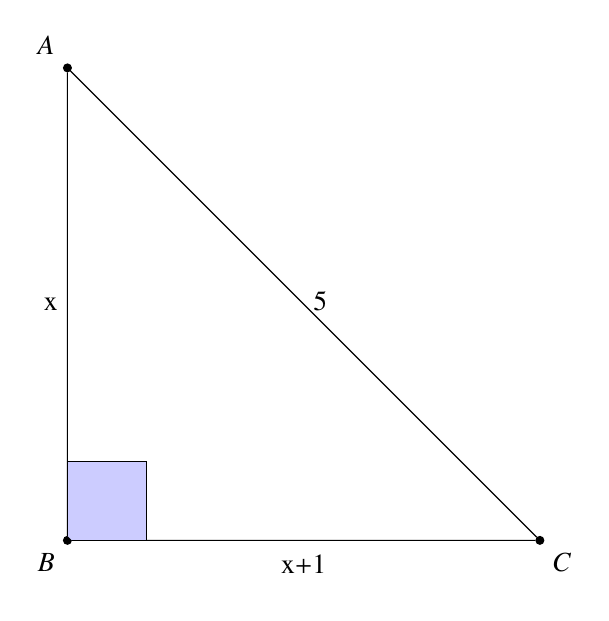
\begin{tikzpicture}
[
 scale=2,
  >=stealth,
  point/.style = {draw, circle, fill = black, inner sep = 1pt},
]

\node (B) at (0,0) [point,label = below left:$B$] {};
\node (A) at (0,3)[point,label = above left:$A$] {};
\node (C) at (3,0)[point,label = below right:$C$] {};
\draw (A) -- (B) -- (C) -- (A);

\tkzMarkRightAngle[fill=blue!20,size=0.5](A,B,C)

\node [left] at (0,1.5) {\strut x};
\node [below] at (1.5,0) {\strut x+1};
\node [right] at (1.5,1.5) {\strut 5};




\end{tikzpicture}

}
\caption{Area of $\Delta ABC= \frac{1}{2} AB \times BC$.}
\label{fig:rt_triang}
\end{figure}

\begin{problem}
Verify that the area of $\Delta ABC \triangleq \frac{1}{2}AB\times BC$. Draw various such triangles and find their area.
\end{problem}
%
\begin{problem}
The figure  in Fig.\ref{fig:square} is a {\em square} where all the sides are equal. Draw it using a scale and protractor.  Note that all angles in the square are $90^{\degree}$.  Find its area given by $AB \times AB = AB^2$.
\end{problem}
%
%
\begin{figure}[!h]
\centering
\resizebox {\columnwidth} {!} {
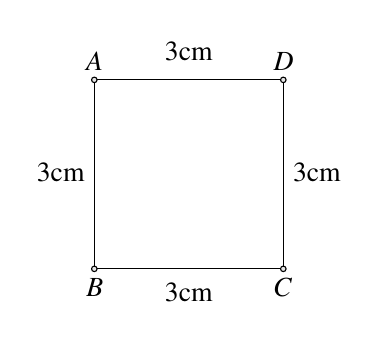
\begin{tikzpicture}[scale=.8]

\tkzDefPoint(0,0){B} \tkzDefPoint(3,0){C}
\tkzDefPoint(3,3){D} \tkzDefPoint(0,3){A}

\draw (0,0) rectangle (3,3);
\tkzDrawPoints(A,B,C,D)
\tkzLabelPoints[below](C,B)
\tkzLabelPoints[above](A,D)
%\tkzMarkRightAngle[fill=blue!20,size=0.5](A,B,C)

\node [left] at (0,1.5) {\strut 3cm};
\node [below] at (1.5,0) {\strut 3cm};
\node [right] at (3,1.5) {\strut 3cm};
\node [above] at (1.5,3) {\strut 3cm};


\end{tikzpicture}
}
\caption{Area of the square$= AB \times AB = AB^2$.}
\label{fig:square}
\end{figure}
%
\begin{problem}
In $\Delta ABC$ in Fig. \ref{fig:rt_triang}, verify that 
%the area of the square on the side $AC = $ area of the square on the side $AB + $area of the square on the side $BC$, or
\begin{equation}
\label{eq:baudhayana}
AC^2 = AB^2 + BC^2
\end{equation}
\end{problem}
\begin{problem}
In the Figure \ref{fig:quad_area}, $BCDF$ is a rectangle with CD = 6cm and DF = 8cm.  Choose points $A$ and $E$ on the line $DF$ such that $AE = BC = 8$cm.  Join $AB$ and $CE$.  The figure $ABCE$ is known as a {\em parallelogram}, denoted as $\parallel^{gm}$. 
\end{problem}
\begin{figure}[!h]
\centering
\resizebox {\columnwidth} {!} {
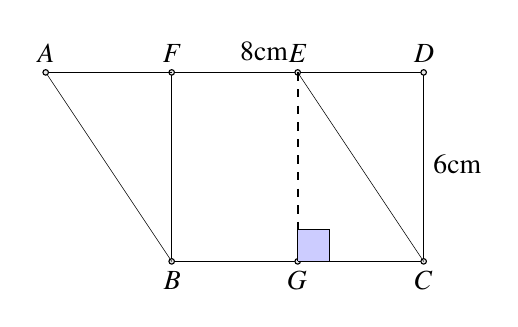
\begin{tikzpicture}[scale=.8]

\tkzDefPoint(0,0){B} \tkzDefPoint(4,0){C}
\tkzDefPoint(4,3){D} \tkzDefPoint(0,3){F}

\draw (0,0) rectangle (4,3);
\tkzDrawPoints(F,B,C,D)
\tkzLabelPoints[below](C,B)
\tkzLabelPoints[above](F,D)


\node [right] at (4,1.5) {\strut 6cm};
\node [left] at (2,3.3) {\strut 8cm};

\tkzDefPoint(2,3){E}
\tkzDefPoint(-2,3){A}
\tkzDrawSegments(E,C A,B A,F)
\tkzDrawPoints(E,A)
\tkzLabelPoints[above](E,A)

\tkzDefPoint(2,0){G}
\tkzDrawPoints(G)
\tkzLabelPoints[below](G)
\draw [thick,dashed] (E) -- (G);
\tkzMarkRightAngle[fill=blue!20,size=0.5](E,G,C)

\end{tikzpicture}


}
\caption{Area of the parallelogram$= BC \times BF$.}
\label{fig:quad_area}
\end{figure}
%
\begin{problem}
Verify that the area
\begin{align}
 \parallel^{gm} ABCE & = \Delta ABF +  \text{rect}BGEF  + \Delta EGC
\\
&= \text{rect}ABCE  = BC \times BF
\end{align}
\end{problem}
%
%\begin{problem}
%Obtain a formula for finding the area of a parallelogram.
%\end{problem}
%
\begin{problem}
Draw Figure \ref{fig:pi} using a compass.  This is known as a {\em circle} with {\em centre} $O$ and {\em radius} $r = 3$cm.  $AB = 2r$ is known as the {\em diameter} of the circle.
\end{problem}
\begin{figure}[!h]
\centering
\resizebox {\columnwidth} {!} {
\begin{tikzpicture}
[
scale =2,
>=stealth,
point/.style = {draw, circle, fill = black, inner sep = 1pt},
]
\def\rad{3}
\coordinate [point, label={below : $O$ }] (O) at (0, 0);
\draw (O) circle (\rad);
\node (B) at +(20:{\rad}) [point,label = above right:$B$] {};
\path
    (O) edge node[sloped, anchor=centre, below, text width=2cm] { $3cm$}  (B);
    
\node (A) at +(200:{\rad}) [point,label = above left:$A$] {};
\path
    (O) edge node[sloped, anchor=centre, below, text width=2cm] { $3cm$}  (A);

\end{tikzpicture}
}
\caption{Circle}
\label{fig:pi}
\end{figure}
\begin{problem}
Draw the circle in Fig. \ref{fig:semi_circle}  with $AC$ as the diameter.  Take any point $B$ on the circle.  Verify that $\angle ABC = 90^{\degree}$ 
\begin{enumerate}
\item Using \eqref{eq:baudhayana}.
\item Using a protractor.
\end{enumerate}
\end{problem}

\begin{figure}[!h]
\centering
\resizebox {\columnwidth} {!} {
\begin{tikzpicture}
  [
    scale=2,
    >=stealth,
    point/.style = {draw, circle, fill = black, inner sep = 1pt},
   ]
 \def\rad{3}
 \coordinate [point, label={below: $O$}] (O) at (0, 0);
 \draw (O) circle (\rad);
 \node (C) at +(20:{\rad}) [point,label = above right:$C$] {};
 \node (A) at (200:{\rad}) [point,label = below left:$A$] {};
 \node (B) at +(100:{\rad}) [point,label = above left:$B$] {};
 \path
     (A) edge node[sloped, anchor=east, below right, text width=1cm] {$3cm$} (O) ;
 \draw (A) -- (C);
 \draw (B) -- (C);
 \draw (A) -- (B);
 
 \path
    (O) edge node[sloped, anchor=east, below right, text width=1cm] {$3cm$} (C) ;
 
 \tkzMarkRightAngle[fill=blue!20,size=.3](A,B,C)



\end{tikzpicture}
}
\caption{Angle in a semi circle $= 90^{\degree}$.}
\label{fig:semi_circle}
\end{figure}
%
\begin{problem}
Draw a line such that it touches the circle in Fig. \ref{fig:tangent}  at the point $P$. Verify that the radius $OP \perp$ the tangent using \eqref{eq:baudhayana}.
\end{problem}
%
\begin{figure}[!h]
\centering
\resizebox {\columnwidth} {!} {
\begin{tikzpicture}
[
scale =2,
>=stealth,
point/.style = {draw, circle, fill = black, inner sep = 1pt},
]
\def\rad{2}
\coordinate [point, label={above : $O$ }] (O) at (0, 0);
\draw (O) circle (\rad);

\coordinate [point, label={below :$P$}] (P) at (0,-2);
%\draw (O) -- (P);

\path
    (O) edge node[anchor=centre, below, text width=2cm] {$3cm$}  (P);
    
\draw (P) -- ($(P)!1!-90:(O)$);
\draw (P) -- ($(P)!1!90:(O)$);

\tkzDefPoint (1,-2){A}
%\tkzLabelPoints(A)

\tkzMarkRightAngle[fill=blue!20,size=.2](O,P,A)

\end{tikzpicture}
}
\caption{Tangent to the circle.}
\label{fig:tangent}
\end{figure}
%
%
\begin{problem}
In $ \Delta ABC$ in Fig. \ref{fig:altitude}, $BE \perp AC$ and $CF \perp AB$ are defined as the {\em altitudes}.  Show that 
\begin{equation}
\text{area of } \Delta ABC = \frac{1}{2}BE \times AC = \frac{1}{2} AB \times CF
\end{equation}
\end{problem}
%
\begin{figure}[!h]
\centering
\resizebox {\columnwidth} {!} {
\begin{tikzpicture}
[
 scale=2,
  >=stealth,
  point/.style = {draw, circle, fill = black, inner sep = 1pt},
]

\node (B) at (-2,-2) [point,label = below left:$B$] {};
\node (A) at (1,3)[point,label = above left:$A$] {};
\node (C) at (4,-1)[point,label = below right:$C$] {};
\draw (A) -- (B) -- (C) -- (A);

\node (E) at (2.32,1.24) [point,label = above:$E$] {};
\draw (B) -- (E);
\tkzMarkRightAngle[fill = blue!20,size=.2](B,E,C)

\node (D) at (1.72972973,-1.37837838)[point,label = below:$D$] {};
\draw [thick,dashed] (A) -- (D);
\tkzMarkRightAngle[fill = blue!40,size=.2](A,D,C)

\node (F) at (0.02941176,1.38235294)[point,label = above:$F$] {};
\draw (C) -- (F);
\tkzMarkRightAngle[fill = blue!60,size=.2](A,F,C)

\node (O) at (1.40741,0.555556) [point,label = above left:$O$] {};

\end{tikzpicture}
}
\caption{Altitudes of a triangle meet in a point.}
\label{fig:altitude}
\end{figure}
%
\begin{problem}
$BE$ and $CF$ in Fig. \ref{fig:altitude} meet at $O$.  Extend $AO$ to meet $BC$ at $D$. Verify that $AD$ is also an altitude of the $\Delta ABC$.
\end{problem}
%
\begin{problem}
Draw the line $BE$ such that it divides the side $AC$ into two equal parts in $ \Delta ABC$ as shown in Fig. \ref{fig:median}. $BE$ is known as the {\em median}.  $CF$ is another median.
$BE$ and $CF$ meet at $O$.  Verify that
\begin{equation}
\frac{OE}{OB} = \frac{OF}{OC} = \frac{1}{2}
\end{equation}
\end{problem}
%
\begin{figure}[!h]
\centering
\resizebox {\columnwidth} {!} {
\begin{tikzpicture}
 [
  scale=2,
  >=stealth,
  point/.style = {draw, circle, fill = black, inner sep = 1pt},
  ]
  
\node (B) at (-2,-2) [point,label = below right:$B$] {};
\node (A) at (1,3) [point,label = above left:$A$] {};
\node (C) at (4,-1) [point,label = below left:$C$] {};
\draw (A) -- (C);
\draw (B) -- (C);
\draw (A) -- (B);

\node (E) at (2.5,1) [point,label = right:$E$] {};
\node (D) at (1,-1.5) [point,label = above right:$D$] {};
\node (F) at (-0.5,0.5) [point,label = above left:$F$] {};
\draw [thick,dashed] (A) -- (D);
\draw (B) -- (E);
\draw (C) -- (F);

\node (O) at (1,0) [point,label = below right:$O$] {};

\node [below] at (1,-1.5) {\strut a};
 
\node [below] at (3.5,0.112) {\strut b/2};

\node [below] at (2.2,2) {\strut b/2};  
 
\node [below] at (-1,-0.5) {\strut c/2}; 
 
\node [below] at (0,2) {\strut c/2}; 
    

\end{tikzpicture}
}
\caption{Medians of a triangle meet in a point.}
\label{fig:median}
\end{figure}
%
\begin{problem}
Extend the line $AO$ in Fig. \ref{fig:median} to meet $BC$ at $D$.  Verify that $AD$ is also a median.
\end{problem}
%
%
\begin{problem}
In $ \Delta ABC$ in Fig. \ref{fig:similar}, mark the mid points of $BC, AC$ and $AB$ respectively as $D,E$ and $F$. 
Verify that
\medskip
\begin{enumerate}
\item
$
\dfrac{EF}{BC} = \dfrac{DE}{AB} = \dfrac{DF}{AC} = \dfrac{1}{2}
$
\medskip
\item 
$
\dfrac{\text{Area of } \Delta DEF}{\text{Area of } \Delta ABC} = \dfrac{1}{4}
$
\medskip
\item 
$
\angle EDC = \angle DEF
$
\medskip
\item
$
{EF}\parallel{BC} = {DE}\parallel{AB} = {DF}\parallel{AC} 
$
\medskip
\item $\Delta DEF \sim \Delta ABC$ .
\end{enumerate}

\end{problem}
%
\begin{figure}[!h]
\centering
\resizebox {\columnwidth} {!} {
\begin{tikzpicture}
 [
  scale=2,
  >=stealth,
  point/.style = {draw, circle, fill = black, inner sep = 1pt},
  ]
  
\node (B) at (-2,-2) [point,label = below right:$B$] {};
\node (A) at (1,3) [point,label = above left:$A$] {};
\node (C) at (4,-1) [point,label = below left:$C$] {};
\draw (A) -- (C);
\draw (B) -- (C);
\draw (A) -- (B);

\node (E) at (2.5,1) [point,label = right:$E$] {};
\node (D) at (1,-1.5) [point,label = below right:$D$] {};
\node (F) at (-0.5,0.5) [point,label = above left:$F$] {};

\draw (E) -- (D);
\draw (F) -- (E);
\draw (D) -- (F);

\node [below] at (-0.5,-1.78) {\strut a/2};
\node [below] at (3,-1.25) {\strut a/2};
      
\node [below] at (-1.7,-1) {\strut c/2};   
\node [below] at (0,2) {\strut c/2};     


\node [below] at (2.1,2) {\strut b/2};
\node [below] at (3.6,0) {\strut b/2};
 
\node [above] at (1,0.78) {\strut a/2};
    
\node [below] at (-0.2,-0.35) {\strut b/2};
    
\node [below] at (2,0) {\strut c/2};    



\end{tikzpicture}
}
\caption{Similar Triangles}
\label{fig:similar}
\end{figure}

\begin{problem}
Draw any circle with {\em diameter AB} as shown in Fig. \ref{fig:pi} and verify that
\begin{equation}
\frac{\text{circumference}}{\text{diameter}} = \pi \approx \frac{22}{7}
\end{equation}
%
Repeat this exercise for circles of different radii.
\end{problem}
%
\begin{problem}
The area of a circle is given by $\pi r^2$.  Calculate the areas of various circles of different radii.
\end{problem}
%
\begin{problem}
Draw the {\em chords} $AB$ and $CD$ meeting at $P$ as shown in Fig. \ref{fig:circle_ratio}.  Join $AC$ and $BD$ and verify that $\Delta PAC \sim \Delta PDB$.
\end{problem}
%
\begin{figure}[!h]
\centering
\resizebox {\columnwidth} {!} {
\begin{tikzpicture}
[
scale =2,
>=stealth,
point/.style = {draw, circle, fill = black, inner sep = 1pt},
]
\def\rad{3}
\coordinate [point, label={below : $O$ }] (O) at (0, 0);
\draw (O) circle (\rad);

\coordinate [point, label={left :$P$}] (P) at (0,-1.5);
\node (D) at +(17:{\rad}) [point,label = above right:$D$] {};

\draw (P) -- (D);
  
\node(C) at +(243:{\rad}) [point,label = left:$C$] {};

\draw (P) -- (C);

\node (A) at +(163:{\rad}) [point,label = above left:$A$] {};

\draw (P) -- (A);

\node (B) at +(-62:{\rad}) [point,label =right:$B$] {};

\draw (P) -- (B);

\end{tikzpicture}
}
\caption{$\Delta PAC \sim \Delta PDB$}
\label{fig:circle_ratio}
\end{figure}
%
\begin{problem}
Now join the lines $OB$ and $OC$ in Fig. \ref{fig:circle_ratio}  and verify that
\begin{equation}
\angle BOC = 2 \angle BDC = 2\angle BAC
\end{equation}
\end{problem}
%
%
\begin{problem}
Draw the tangent through the point $B$ and $\Delta ABC$ as in Fig. \ref{fig:tangent_angle}.  Verify that the marked angles are equal.
\end{problem}
%
\begin{figure}[!h]
\centering
\resizebox {\columnwidth} {!} {
\begin{tikzpicture}
[
scale =2,
>=stealth,
point/.style = {draw, circle, fill = black, inner sep = 1pt},
]
\def\rad{3}
\coordinate [point, label={above : $O$ }] (O) at (0, 0);
\draw (O) circle (\rad);

\coordinate [point, label={below :$B$}] (B) at (0,-3);
%\node (B) at (270:{\rad})[point,label = below:$B$] {};

\draw (B) -- ($(B)!1!-90:(O)$);
\draw (B) -- ($(B)!1!90:(O)$);


\node (A) at (130:{\rad}) [point,label = left:$A$] {};
\draw (A) -- (B);

\node (C) at (340:{\rad}) [point,label = right:$C$] {};
\draw (C) -- (A);
\draw (B) -- (C);


\tkzMarkAngle[fill=blue!40,size=.3](B,A,C)
\tkzDefPoint (2,-3){P}
\tkzLabelPoints(P)
\tkzMarkAngle[fill=blue!40,size=.3](P,B,C)


\end{tikzpicture}
}
\caption{Angles in the figure are equal.}
\label{fig:tangent_angle}
\end{figure}
%
%
\begin{problem}
Draw the tangent $PT$ to the circle as shown in  Fig. \ref{fig:tangent_intercept} and a line $PAB$ intersecting the circle at points $A$ and $B$.  Verify that
\begin{equation}
PA\times PB = PT^2
\end{equation}
\end{problem}
%
\begin{figure}[!h]
\centering
\resizebox {\columnwidth} {!} {
\begin{tikzpicture}
[
scale =2,
>=stealth,
point/.style = {draw, circle, fill = black, inner sep = 1pt},
]
\def\rad{3}
\coordinate [point, label={above : $O$ }] (O) at (0, 0);
\draw (O) circle (\rad);

\coordinate [point, label={below :$T$}] (T) at (0,-3);

\draw (T) -- ($(T)!1!-90:(O)$);
\draw (T) -- ($(T)!1!90:(O)$);

\tkzDefPoint (-3,-3){P}
\tkzLabelPoints(P)

\node (A) at (215:{\rad}) [point,label = left:$A$] {};
 \node (B) at +(100:{\rad}) [point,label = above left:$B$] {};
 
 \draw (P) -- (B);



\end{tikzpicture}
}
\caption{$PA\times PB = PT^2$.}
\label{fig:tangent_intercept}
\end{figure}
%
%
\begin{problem}
In Fig. \ref{fig:tangent_equal} draw tangents $PA$ and $PB$ to the circle where $P$ is any point outside the circle. Verify that $PA = PB$.
\end{problem}
%
\begin{figure}[!h]
\centering
\resizebox {\columnwidth} {!} {
\begin{tikzpicture}
[
scale =2,
>=stealth,
point/.style = {draw, circle, fill = black, inner sep = 1pt},
]
\def\rad{2}
\coordinate [point, label={above : $O$ }] (O) at (0, 0);
\draw (O) circle (\rad);


\node (A) at (140:{\rad}) [point,label = left:$A$] {};
 \node (B) at +(40:{\rad}) [point,label = right:$B$] {};
 
 \coordinate [point, label={above : $P$}] (P) at (0,3.5);
 
 \draw (P) -- (A);
 \draw (P) -- (B);

\end{tikzpicture}
}
\caption{$PA=PB$.}
\label{fig:tangent_equal}
\end{figure}
%
%
\begin{problem}
In Fig. \ref{fig:ang_bisect} draw the {\em angle bisectors} $BD$ and $CF$ such that 
%
\begin{align}
\angle ABD &= \angle CBD
\\
\angle ACF &= \angle BCF
\end{align}
%
Verify that the line $AO$ is also  an angle bisector.
\end{problem}
%
\begin{figure}[!h]
\centering
\resizebox {\columnwidth} {!} {
\begin{tikzpicture}
[
 scale=2,
  >=stealth,
  point/.style = {draw, circle, fill = black, inner sep = 1pt},
]

\node (B) at (-2,-2)[point,label = below left:${B}$] {};
\node (A) at (1,3)[point,label = above left:${A}$] {};
\node (C) at (4,-1)[point,label = below right:${C}$] {};
\draw (A) -- (B) -- (C) -- (A);

\node (D) at (2.4682957,1.0422724)[point,label = above right:$D$] {};
\draw (B) -- (D);


\node (E) at (1.23016035,-1.46163994)[point,label = below:$E$] {};
%\draw (A) -- (E);
\draw[thick, dashed] (A) -- (E);


\node (F) at (-0.35345316,  0.74424473)[point,label = left:$F$] {};
\draw (C) -- (F);

\node (O) at (1.14738665, 0.14292163) [point,label = right:$O$] {};

\tkzMarkAngle[fill=blue!60,size=.3](O,B,F)
\tkzMarkAngle[fill=blue!40,size=.3](E,B,O)


\tkzMarkAngle[fill=red!60,size=.3](F,A,O)
\tkzMarkAngle[fill=red!40,size=.3](O,A,D)


\tkzMarkAngle[fill=orange!60,size=.3](D,C,O)
\tkzMarkAngle[fill=orange!40,size=.3](O,C,E)


\end{tikzpicture}
}
\caption{Angles bisectors meet at a point.}
\label{fig:ang_bisect}
\end{figure}
%
%
\begin{problem}
In Fig. \ref{fig:perp_bisect} draw the {\em perpendicular bisectors} $BD$ and $CE$ meeting at the point $O$. Draw $OD$ perpendicular to $BC$.  Verify that $BD=DC$.
\end{problem}
%
\begin{figure}[!h]
\centering
\resizebox {\columnwidth} {!} {
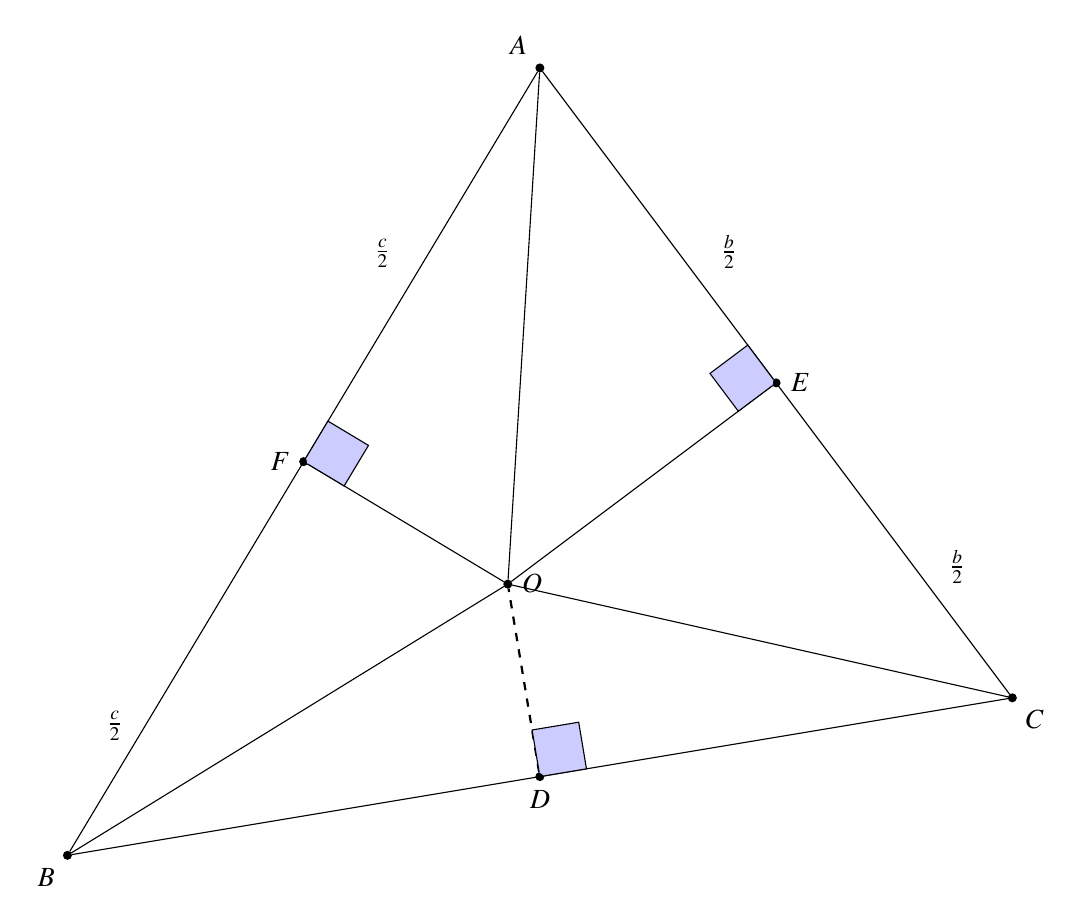
\begin{tikzpicture}
[
 scale=2,
  >=stealth,
  point/.style = {draw, circle, fill = black, inner sep = 1pt},
]
\node (B) at (-2,-2)[point,label = below left:${B}$] {};
\node (A) at (1,3)[point,label = above left:${A}$] {};
\node (C) at (4,-1)[point,label = below right:${C}$] {};
\draw (A) -- (B) -- (C) -- (A);

\node (D) at (1,-1.5)[point,label = below:$D$] {};

\node (F) at (-0.5,0.5)[point,label = left:$F$] {};

\node (E) at (2.5,1)[point,label = right:$E$] {};

\node (O) at (0.7962963,-0.27777778) [point,label = right:$O$] {};

\draw[thick, dashed] (D) -- (O);
\draw (F) -- (O);
\draw (E) -- (O);
\draw (A) -- (O);
\draw (B) -- (O);
\draw (C) -- (O);

\tkzMarkRightAngle[fill=blue!20,size=.3](A,E,O)
\tkzMarkRightAngle[fill=blue!20,size=.3](A,F,O)
\tkzMarkRightAngle[fill=blue!20,size=.3](O,D,C)


\node [below] at (3.65,0) {\strut $\frac{b}{2}$};
\node [below] at (2.2,2) {\strut  $\frac{b}{2}$};


%\node [below] at (2.5,-1.2) {\strut a/2};    
%\node [below] at (0,-1.65) {\strut a/2};  
      
\node [below] at (-1.7,-1) {\strut  $\frac{c}{2}$}; 
\node [below] at (0,2) {\strut  $\frac{c}{2}$};   


\end{tikzpicture}

}
\caption{Perpendicular bisectors meet at a point.}
\label{fig:perp_bisect}
\end{figure}
%
%\newpage
%\section{Natural Numbers}
%%%
%%
%\renewcommand{\theequation}{\theenumi}
\begin{enumerate}[label=\arabic*.,ref=\thesubsection.\theenumi]
\numberwithin{equation}{enumi}
%\chapter{The Optimum Receiver}

%\subsection{Problem}
\item


A right angled triangle looks like Fig. \ref{ch1_right}.
\begin{figure}[!ht]
\begin{center}
	
%\includegraphics[width=\columnwidth]{./figs/right_angle_tri.tex}
\resizebox{\columnwidth}{!}{
\begin{tikzpicture}[scale=2]%,cap=round,>=latex]

\coordinate [label=left:$B$] (A) at (-1.5cm,-1.0cm);
\coordinate [label=right:$C$] (C) at (1.5cm,-1.0cm);
\coordinate [label=above:$A$] (B) at (1.5cm,1.0cm);
\draw (A) -- node[sloped,above] {$\textrm{c}$} (B) -- node[above,xshift=2mm] {$\textrm{b}$} (C) -- node[below] {$\textrm{a}$} (A);

\draw (1.25cm,-1.0cm) rectangle (1.5cm,-0.75cm);
\tkzMarkAngle[size=0.5cm,color=black,mark=](C,A,B) 
\tkzLabelAngle[pos=0.65](C,A,B){$\theta$}
\end{tikzpicture}}
%\vspace*{-10cm}
\end{center}
\caption{Right Angled Triangle}
\label{ch1_right}	
\end{figure}
%\vspace*{-10cm}
with angles $\angle A,\angle B$ and $\angle C$ and sides $a, b$ and $c$.  The unique feature of this triangle is $\angle C$ which is defined to be $90^{\degree}$.
\item
	For simplicity, let the greek letter $\theta = \angle B$.  We have the following definitions.
\begin{equation}
\label{ch1_trig_defs}
\begin{matrix}
	\sin \theta = \frac{a}{c} & 	\cos \theta = \frac{b}{c} \\
	\tan \theta = \frac{b}{a} & \cot \theta = \frac{1}{\tan \theta} \\
	\csc \theta = \frac{1}{\sin \theta} & \sec \theta = \frac{1}{\cos \theta}
	\end{matrix}
\end{equation}
\end{enumerate}

\subsection{Sum of Angles}
\renewcommand{\theequation}{\theenumi}
\begin{enumerate}[label=\arabic*.,ref=\thesubsection.\theenumi]
\numberwithin{equation}{enumi}
\item 	In Fig. \ref{ch1_parallel_triangle}, the sum of all the angles on the top or bottom side of the straight line $XY$ is $180^{\degree}$.


\begin{figure}[!ht]
	\begin{center}
		\resizebox{\columnwidth}{!}{\begin{tikzpicture}
[scale=2,>=stealth,point/.style={draw,circle,fill = black,inner sep=0.5pt},]

\node (A) at (0, 0)[point,label=above right:$A$] {};
\node (Y) at (2, 0)[point,label=above right:$Y$] {};
\node (X) at (-2, 0)[point,label=above right:$X$] {};
\node (T) at (0, 1)[point,label=above right:$T$] {};
\node (V) at (-1.2, 1)[point,label=above right:$V$] {};
\node (C) at (0, -3)[point,label=below right:$C$] {};
\node (B) at (3.5, -3)[point,label=above right:$B$] {};
\draw (Y)--(A);
\draw (X)--(A);
\draw (T)--(A);
\draw (V)--(A);
\draw (C)--(A);
\draw (B)--(A);
\draw (B)--(C);

\tkzMarkAngle[size=.3](A,B,C)
\tkzMarkAngle[size=.3](V,A,X)
\tkzMarkAngle[size=.3](C,A,B)
\draw (-0.4,0.1) node{$\theta$};
\draw (3.1,-2.9)[label=below] node{$\theta$};
\tkzMarkRightAngle[size=.2](B,C,A)
\tkzMarkRightAngle[size=.2](C,A,X)

\node [below] at (1.7,-3.1) {$a$};
\node  at (-0.1,-1.5) {$b$};
\node at (2,-1.5) {$c$};

\end{tikzpicture}}
		%
\includegraphics[width=\columnwidth]{./figs/ch1_parallel_triangle}
		%\vspace*{-10cm}
	\end{center}
	\caption{Sum of angles of a triangle}
	\label{ch1_parallel_triangle}	
\end{figure}



\item
In Fig. \ref{ch1_parallel_triangle}, the straight line making an angle of $90^{\degree}$ to the side $AC$ is said to be parallel to the side $BC$. Note there is an angle at $A$ that is equal to $\theta$.  This is one property of parallel lines.  Thus, $\angle YAZ = 90^{\degree}$.


\item
	Show that $\angle VAZ = 90^{\degree} - \theta$
		
	\proof Considering the line $XAZ$,
	\begin{align}
	\theta + 90^{\degree} + \angle VAZ &= 180^{\degree} \\
	\Rightarrow  \angle VAZ =  90^{\degree} - \theta
	\end{align}

\item
	\label{ch1_compl_angle}
	Show that $\angle BAC = 90^{\degree} - \theta$.
	
	\proof Consider the line $VAB$ and and use the approach in the previous problem.  Note that this implies that $\angle VAZ = \angle BAC$.  Such angles are known as vertically opposite angles. 
	 
\item
Sum of the angles of a triangle is equal to $180^{\degree}$
\end{enumerate}
\subsection{Budhayana Theorem}
\renewcommand{\theequation}{\theenumi}
\begin{enumerate}[label=\arabic*.,ref=\thesubsection.\theenumi]
\numberwithin{equation}{enumi}



\item 	Using Fig. \ref{ch1_right}, show that
	\begin{equation}
	\cos \theta = \sin \brak{90^{\degree} - \theta}
	\end{equation}


\begin{figure}[!ht]
	\begin{center}
		
		%
\includegraphics[width=\columnwidth]{./figs/ch1_budh_triangle}
		\resizebox{\columnwidth}{!}{
\begin{tikzpicture}
[scale=2,>=stealth,point/.style={draw,circle,fill = black,inner sep=0.5pt},]
\node (B) at (3, 0)[point,label=above right:$B$] {};
\node (A) at (-1, 3)[point,label=above right:$A$] {};
\node (C) at (-1, 0)[point,label=above left:$C$] {};

\draw (A)--(B);
\draw (B)--(C);
\draw (C)--(A);

\node (D) at (1, 1.5)[point,label= above right:$D$] {};
\draw (D)--(C);
\tkzMarkRightAngle[size=.2](B,C,A)
\tkzMarkRightAngle[size=.2](B,D,C)
\tkzMarkAngle[size=.3](A,B,C)
\tkzMarkAngle[size=.3](C,A,B)
\draw (2.6,0.12) node{$\theta$};
\draw (-.7,2.52) node{$90-\theta$};

\node [above] at (0.9,-0.2) {$a$};
\node [above] at (-1.1,1.2){$b$};
\node [below] at (0.9,1.9){$c$};
\end{tikzpicture}}
		%\vspace*{-10cm}
	\end{center}
	\caption{Budhayana Theorem}
	\label{ch1_budh_triangle}	
\end{figure}


\proof From Problem \ref{ch1_compl_angle} and  \eqref{ch1_trig_defs}
%
\begin{equation}
	\cos \brak{90^{\degree}-\theta} = \frac{b}{c} = \sin \theta
\end{equation}
%
\item
Using Fig. \ref{ch1_budh_triangle}, show that 
%
\begin{equation}
\label{ch1_budh_basic}
c = a \cos \theta + b \sin \theta
\end{equation}
%

\proof We observe that
%
\begin{align}
BD &= a \cos \theta \\
AD &= b \cos\brak{90-\theta} = b \sin \theta \quad \brak{\text{From} \quad \eqref{ch1_compl_angle}}
\end{align}
%
Thus,
\begin{equation}
BD + AD = c = a \cos \theta + b \sin \theta
\end{equation}
\item
From \eqref{ch1_budh_basic}, show that
%
\begin{equation}
\sin ^2 \theta + \cos ^2 \theta = 1
\end{equation}


%
\proof Dividing both sides of \eqref{ch1_budh_basic} by $c$, 
\begin{align}
1 &= \frac{a}{c}\cos\theta + \frac{b}{c}\sin\theta\\
\Rightarrow &\sin ^2 \theta + \cos ^2 \theta = 1 \quad \brak{\text{from} \quad \eqref{ch1_trig_defs}}
\end{align}

\item
	Using \eqref{ch1_budh_basic}, show that
	\begin{equation}
	\label{ch1_budhayana_them}
	c^2 = a^2 + b^2
	\end{equation}
	\eqref{ch1_budhayana_them} is known as the Budhayana theorem.  It is also known as the Pythagoras theorem.

\proof From \eqref{ch1_budh_basic},
\begin{align}
c &= a\frac{a}{c} + b \frac{b}{c} \quad \brak{\text{from} \quad \eqref{ch1_trig_defs}}\\
\Rightarrow c^2 &= a^2 + b^2
\end{align}
\end{enumerate}



%%%
%%
%%%\newpage
%\section{Fractions and Decimals}
%\subsection{Driving the Segments}
%Open the arduino software.  Check if the ports show Arduino Uno and click the appropriate button.  
\begin{problem}
%Connect the A-D pins of the 7447 IC to the pins D2-D5 of the Arduino.
%Connect the A-D pins of the 7447 IC  in Fig. \ref{fig:7447} to the GPIO pins  0-3 of the Pi shown in Figs. \ref{fig_1_3a} and \ref{fig_1_3b}.
\end{problem}	
\renewcommand{\thefigure}{\theproblem.\arabic{figure}}
\begin{figure}[!ht]
\begin{center}
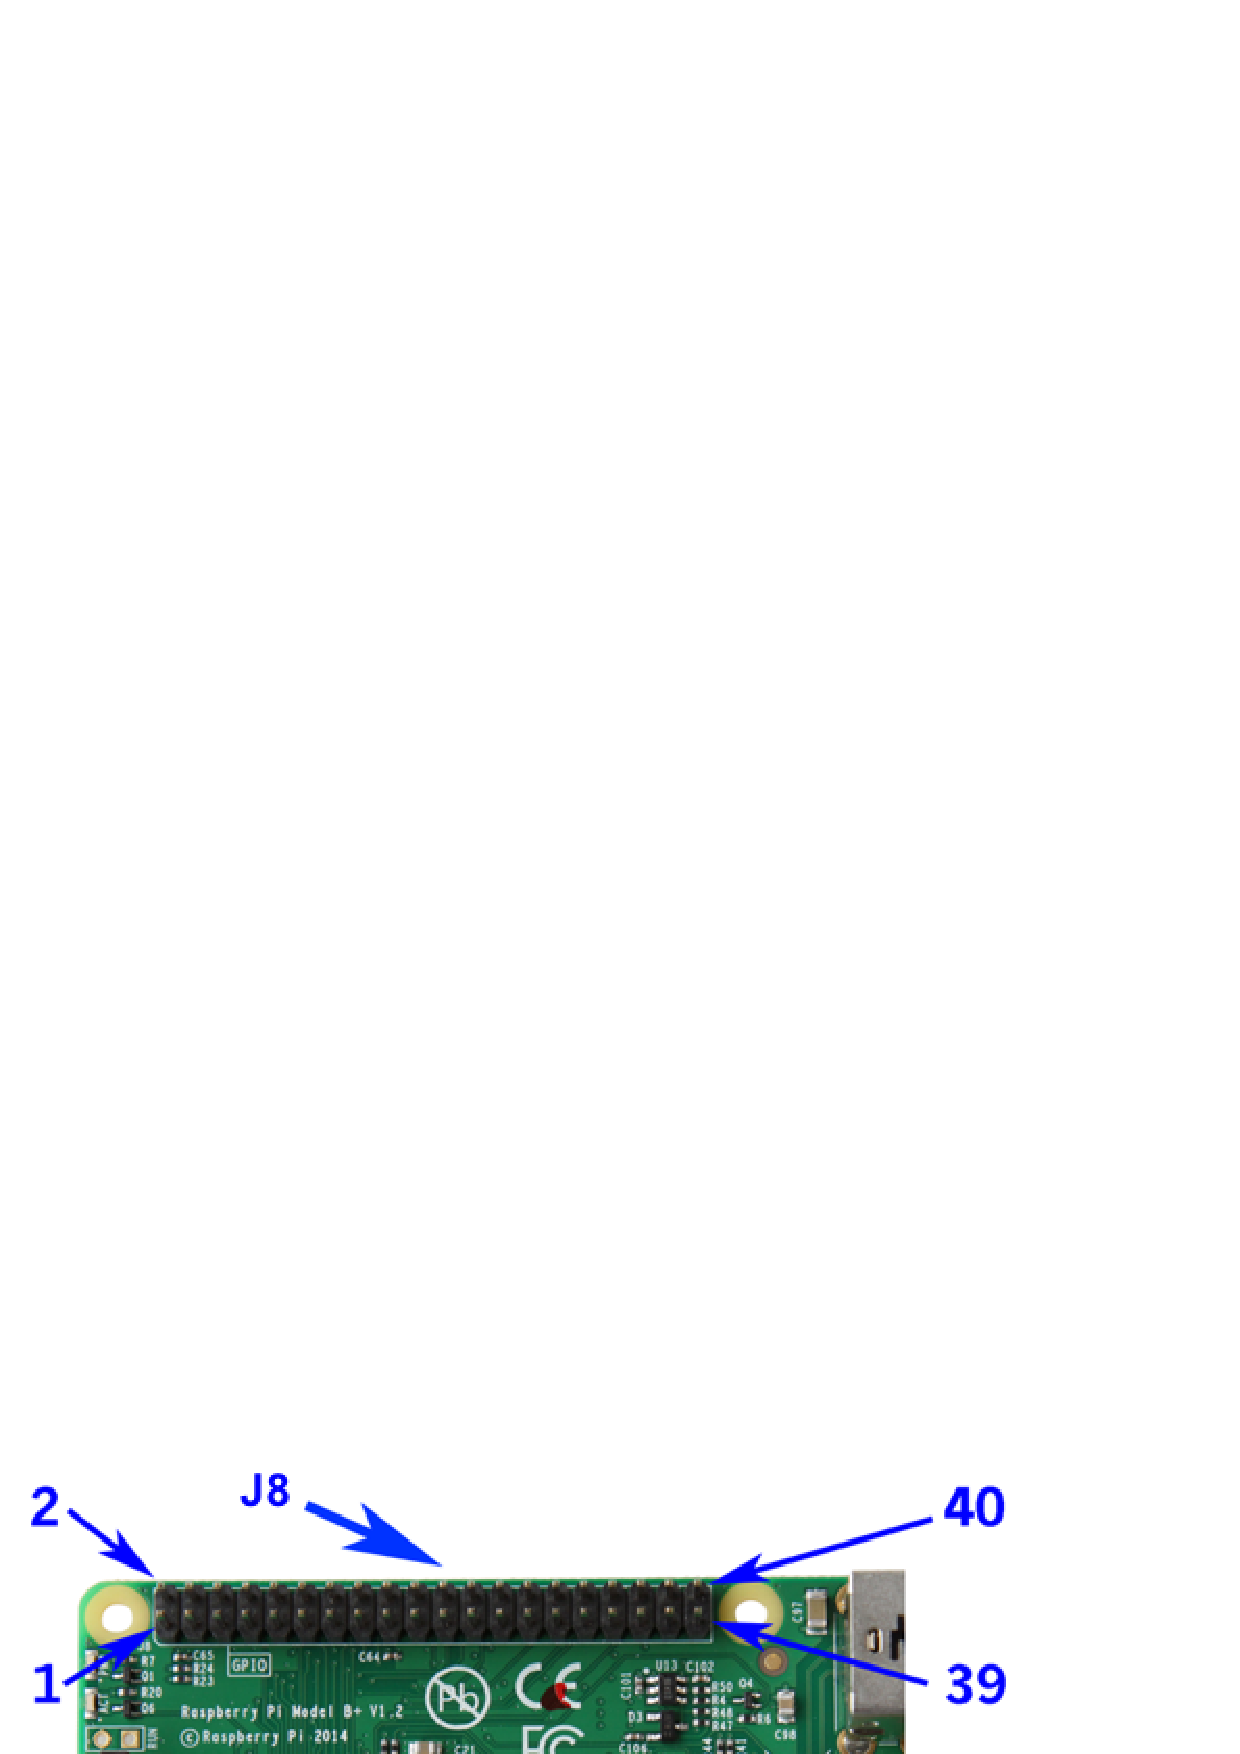
\includegraphics[width=\columnwidth]{./figs/gpio2}
\end{center}
\captionof{figure}{GPIO pin snapshot on Pi.}
\label{fig_1_3a}	
\end{figure}
%
\begin{figure}
\begin{center}
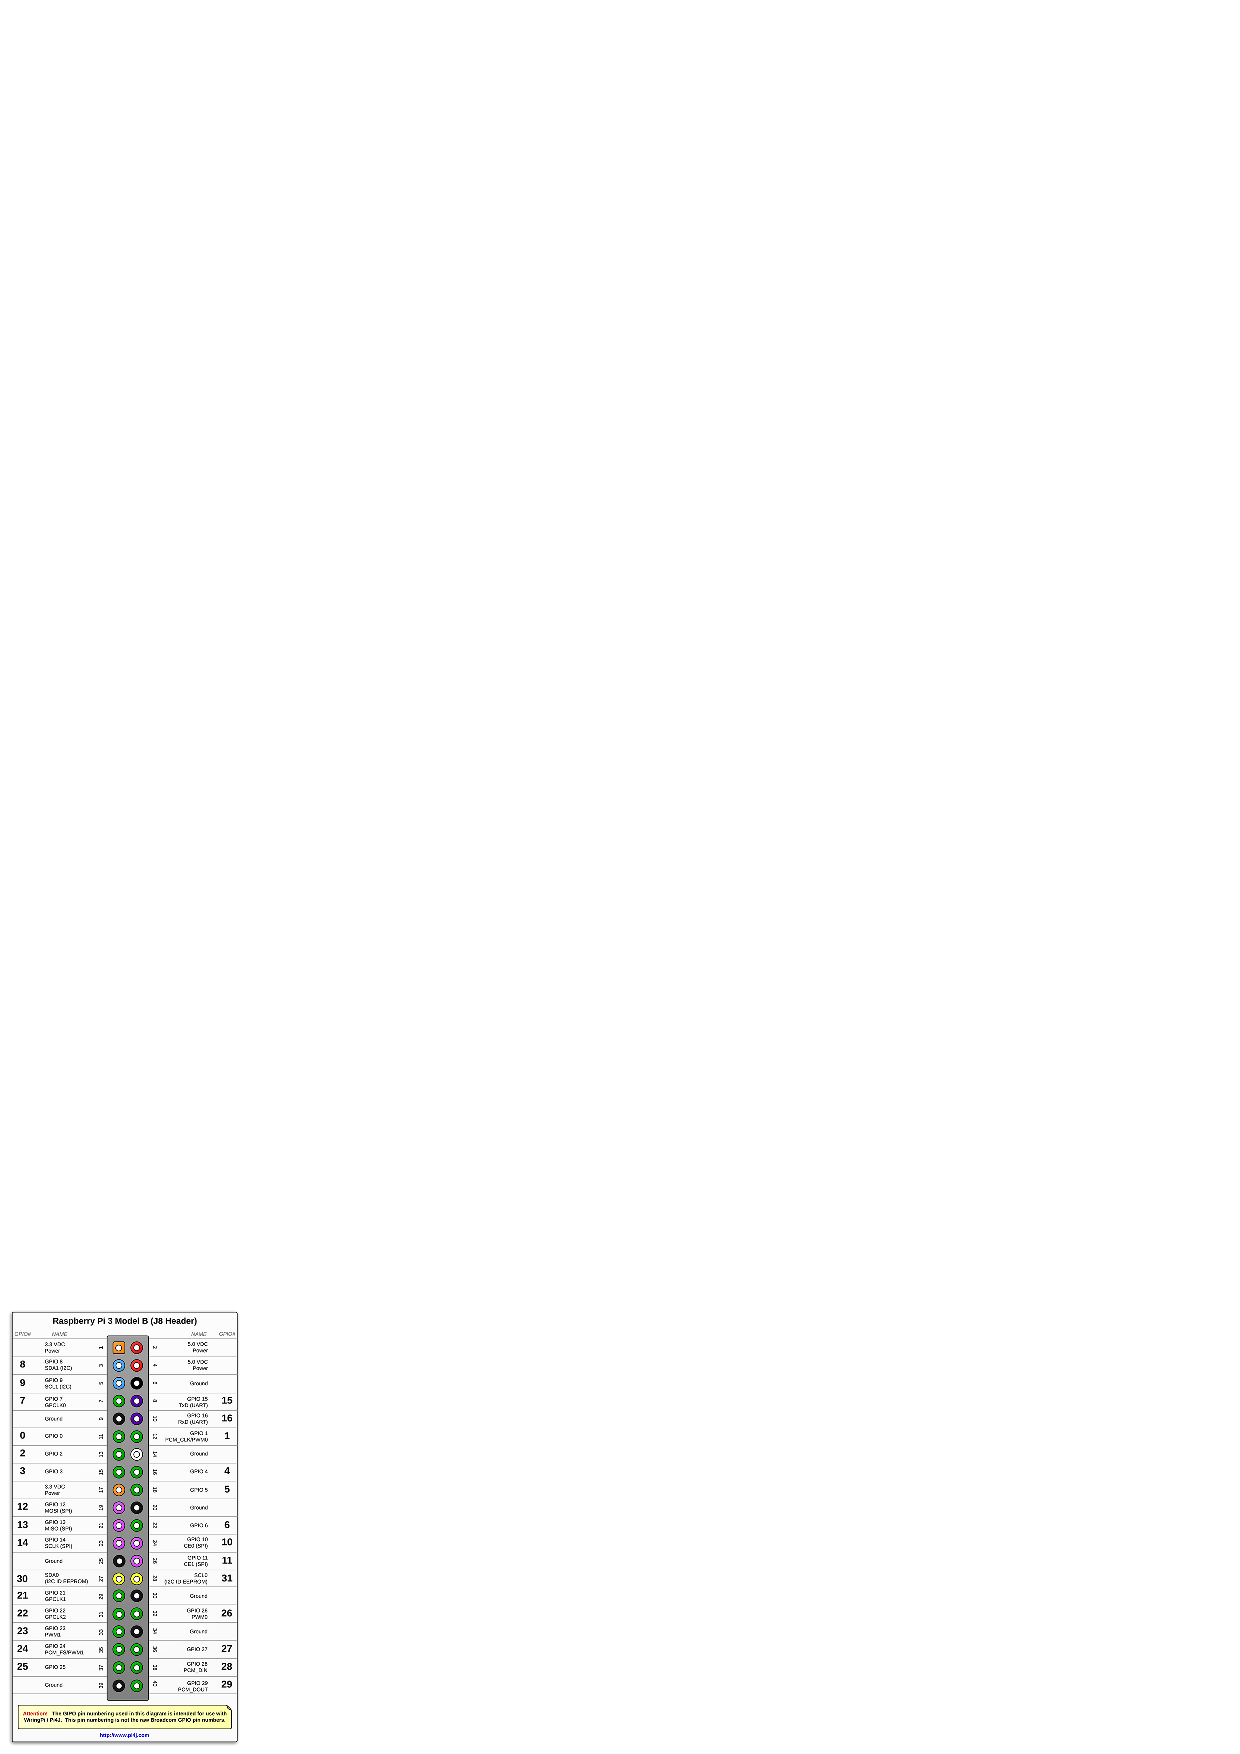
\includegraphics[width=\columnwidth]{./figs/gpio1}
\end{center}
\captionof{figure}{GPIO Wiring Pi pin configuration.}
\label{fig_1_3b}	
\end{figure}
\renewcommand{\thefigure}{\theproblem}
\begin{problem}
Connect the a-g pins of the display to the GPIO pins 0-6 of the Pi shown in \ref{fig_1_3a} and \ref{fig_1_3b}.
\end{problem}
\begin{problem}
Type the following C code and excute. What do you observe?
\end{problem}
\solution
\lstinputlisting[language=C]{./code/seven_seg_disp.c}
\begin{problem}
Now generate the numbers 0-9 by modifying the above program.
\end{problem}
\begin{problem}
Suitably modify the above program to obtain a decade counter.
\end{problem}


%\begin{problem}
%\label{prob:first_code}
%%Type the following code and execute. What do you observe?
%%\lstinputlisting[language=C]{./codes/bcd_seven.c}
%%// the setup function runs once when you press reset or power the board
int a=1,b=0,c=0,d=1,e=1,f=1,g=1;
void setup() {
    pinMode(2, OUTPUT);  
    pinMode(3, OUTPUT);
    pinMode(4, OUTPUT);
    pinMode(5, OUTPUT);
    pinMode(6, OUTPUT);
    pinMode(7, OUTPUT);
    pinMode(8, OUTPUT);            
}

// the loop function runs over and over again forever
void loop() {
  
  digitalWrite(2, a); 
  digitalWrite(3, b); 
  digitalWrite(4, c); 
  digitalWrite(5, d); 
  digitalWrite(6, e); 
  digitalWrite(7, f);     
  digitalWrite(8, g); 
}


%\end{problem}
%\begin{problem}
%Now generate the numbers 0-9 by modifying the above program.
%\end{problem}
%%
%%\newpage

%%\section{Combinational Logic}
%%
%\subsection{Counting Decoder}
	%In the  truth table in Table \ref{table:counter_decoder},  $W,X,Y,Z$ are the inputs
%and $A,B,C,D$ are the outputs. This table represents the system that increments the numbers 0-8 by 1 and resets the number 9 to 0
%%
%Note that  $D = 1$ for the inputs $0111$ and $1000$.  Using {\em boolean} logic,
%%
%\begin{equation}
%\label{bool_logic}
%D = WXYZ^{'} + W^{'}X^{'}Y^{'}Z
%\end{equation}
%%
%Note that $0111$ results in the expression $WXYZ^{'}$ and $1000$ yields $W^{'}X^{'}Y^{'}Z$. 
%%The $\&\&$ operand is used for the boolean AND (multiplication) operation, the $||$ operand is used for the OR (addition) operation and the ! operand is used for the NOT ($^{'}$) operation in Arduino code.  For example, the expression for \eqref{bool_logic} in Arudino is
%%\begin{verbatim}
%%D = (W&&X&&Y&&!Z)||(!W&&!X&&!Y&&Z);
%%\end{verbatim}

%\begin{problem}
	%\label{counter_dec}

%Write the boolean logic functions for $A,B,C$ in terms of $W,X,Y,Z$.
%\end{problem}
%%
%\input{./figs/counter_decoder}
%%
%%
%\begin{problem}
%%	\label{D_code}
%Write a program for implementing Table \ref{counter_dec}.
%%\eqref{bool_logic} in Arduino.
%\end{problem}
%%
%\solution
%%\lstinputlisting[language=C]{./codes/count_decoder.c}
%%
%%\begin{problem}
%%Modify the above program by keeping W=0,X=0,Y=0,Z=1 and A=1 and execute.  Verify that your results are consistent with Table \ref{counter_dec}.
%%\end{problem}

%\begin{problem}
%Verify if your logic is correct by observing the output on the seven segment display for different inputs.
%\end{problem}
%%
%\begin{problem}
%Connect GPIO pin 10 to the dot pin of the display and execute the following code.
%\end{problem}
%%\lstinputlisting[language=C]{./codes/blink.c}
%%
%%
%\begin{problem}
%A decade counter counts the numbers from 0-9 and then resets to 0.  Suitable modify the above programs to obtain a decade counter.
%\end{problem}

%\subsection{Display Decoder}
%%
%\begin{problem}
%Now write the truth table for the seven segment display decoder (IC 7447).  The inputs will be $A,B,C,D$ and the outputs will be $a,b,c,d,e,f,g$.
%\end{problem}
%%
%\begin{problem}
%\label{seven_seg_disp_logic}
%Obtain the logic functions for outputs $a,b,c,d,e,f,g$ in terms of the inputs $A,B,C,D$.
%\end{problem}
%\begin{problem}
%Disconnect the Pi from IC 7447 and connect the pins GPIO 0-6 in the Pi directly to the seven segment display.
%\end{problem}
%\begin{problem}
%Write a new program to implement the logic in Problem \ref{seven_seg_disp_logic} and observe the output in the display.  You have designed the logic for IC 7447!
%\end{problem}
%\begin{problem}
%Now include your counting decoder program in the  display decoder program
%and see if the display shows the consecutive number.
%\end{problem}
%A decade counter counts the numbers from 0-9 and then resets to 0.
%\begin{problem}
%Suitably modify the above program to obtain a decade counter.
%\end{problem}




%\begin{problem}
%Generate the boolean functions for the segments $a-f$ using the table in Problem \ref{bcd_ss}.  For example, the function for $a$ is obtained from the table as
%\begin{equation}
%a=\bar{D}\bar{C}\bar{B}A+\bar{D}C\bar{B}\bar{A}
%\label{boolean}
%\end{equation}
%\end{problem}
%%
%\begin{problem}
	%\label{counter_dec}
%Write functions for $A,B,C,D$ in Arduino using the following table and verify using the Arduino driven display.
		%\input{counter_decoder}
%\end{problem}
%\begin{problem}
	%Write a module for decimal to binary conversion
	%according to the example given below
	%\input{conversion}
	%%
	%$N \% 2$ gives the remainder and $N/2$ gives the quotient
%	and use it in the above code so that decimal values are given as input in the program and observed as output in the display. Note that the following code
%	\begin{verbatim}
%	a % b
%	\end{verbatim}
%	can be used to obtain the remainder when a is divided by b and
%	\begin{verbatim}
%	a/b
%	\end{verbatim}
%	gives the quotient.
%\end{problem}

%\section{Ratio}
%\subsection{Angle Bisectors}

\begin{figure}[!h]
	\begin{center}
		
		%
\includegraphics[width=\columnwidth]{./figs/ch3_angle_bisector}
		%\vspace*{-10cm}
		\resizebox{\columnwidth}{!}{\begin{tikzpicture}
[scale=2,>=stealth,point/.style={draw,circle,fill = black,inner sep=0.5pt},]

\node (D) at (0, 0)[point,label=below :$D$] {};
\node (A) at (0, 3)[point,label=above :$A$]{};
\node (B) at (-3, 0)[point,label=below left:$B$]{};
\node (C) at (3, 0)[point,label=below right:$C$]{};
\node (O) at (0, 1.3)[point,label=below right:$O$]{};
\node (F) at (-1.1, 1.9)[point,label=above left:$F$]{};
\node (E) at (1.1, 1.9)[point,label=above right:$E$]{};

\draw (D)--(B);
\draw (B)--(A);
\draw (A)--(C);
\draw (C)--(D);
\draw [thick,dashed] (A) -- (D);
\draw [thick,dashed] (O) -- (E);
\draw [thick,dashed] (O) -- (F);
\draw (B)--(O);
\draw (C)--(O);

\tkzMarkRightAngle[size=.2](A,D,C)
\tkzMarkRightAngle[size=.15](B,F,O);
\tkzMarkRightAngle[size=.15](C,E,O);
\tkzMarkAngle[size=.4](D,B,O);
\tkzMarkAngle[size=.35](O,B,F);
\tkzMarkAngle[size=.54](E,C,O);
\tkzMarkAngle[size=.5](E,C,O);
\tkzMarkAngle[size=.6](O,C,D);
\tkzMarkAngle[size=.65](O,C,D);

\end{tikzpicture}}
	\end{center}
	\caption{Angle bisectors meet at a point}
	\label{ch3_angle_bisector}	
\end{figure}

\begin{definition}
	In Fig. \ref{ch3_angle_bisector}, $OB$ divides the  $\angle B$ into half, i.e.\begin{equation}
	\angle OBC = \angle OBA
	\end{equation}
	$OB$ is known as an angle bisector.
\end{definition}
	$OB$ and $OC$ are angle bisectors of angles $B$ and $C$. $OA$ is joined and $OD, OF$ and $OE$ are perpendiculars to sides $a,b$ and $c$.
\begin{problem}
  Show that $OD = OE = OF$.
\end{problem}
\proof In $\Delta$s $ODC$ and $OEC$,
\begin{align}
OD &= OC \sin \frac{C}{2}
\\
OE &= OC \sin \frac{C}{2} 
\\
\Rightarrow OD &=OE.
\end{align}
Similarly,
\begin{equation}
OD = OF.
\end{equation}
%
\begin{problem}
	Show that OA is the angle bisector of $\angle A$
\end{problem}
\proof In $\Delta$s $OFA$ and $OEA$,
\begin{align}
OF &= OE
\\
\Rightarrow OA \sin OAF &= OA \sin OAE \\
\Rightarrow \sin OAF &=  \sin OAE \\
\Rightarrow \angle OAF &= \angle OAE
\end{align}
which proves that $OA$ bisects $\angle A$.
{\em Conclusion:} The angle bisectors of a triangle meet at a point.


\subsection{Congruent Triangles}
%
\begin{problem}
	Show that in $\Delta$s $ODC$ and $OEC$, corresponding sides and angles are equal.
\end{problem}
\begin{definition}
	Note that    $\Delta$s $ODC$ and $OEC$ are known as congruent triangles.  To show that two triangles are congruent, it is sufficient to show that some angles and sides are equal.
\end{definition}
\begin{problem}
SSS:	Show that if the corresponding sides of three triangles are equal, the triangles are congruent.
\end{problem}
\begin{problem}
ASA:	Show that if two angles and any one side  are equal in corresponding triangles, the triangles are congruent.
\end{problem}
\begin{problem}
SAS:	Show that if two sides and the angle between them are equal in corresponding triangles, the triangles are congruent.
\end{problem}
\begin{problem}
RHS:	For two right angled triangles, if the hypotenuse and one of the sides are equal, show that the triangles are congruent.
\end{problem}
	%
%%
\subsection{Perpendicular Bisectors}
\begin{definition}
	In Fig. \ref{ch3_perp_bisector}, OD $\perp BC$ and $BD=DC$. $OD$ is defined as the perpendicular bisector of $BC$.
\end{definition}

\begin{problem}
	In Fig. \ref{ch3_perp_bisector}, show that $OA=OB=OC$.
\end{problem}
%%
%%
\begin{figure}[!h]
	\begin{center}
		
		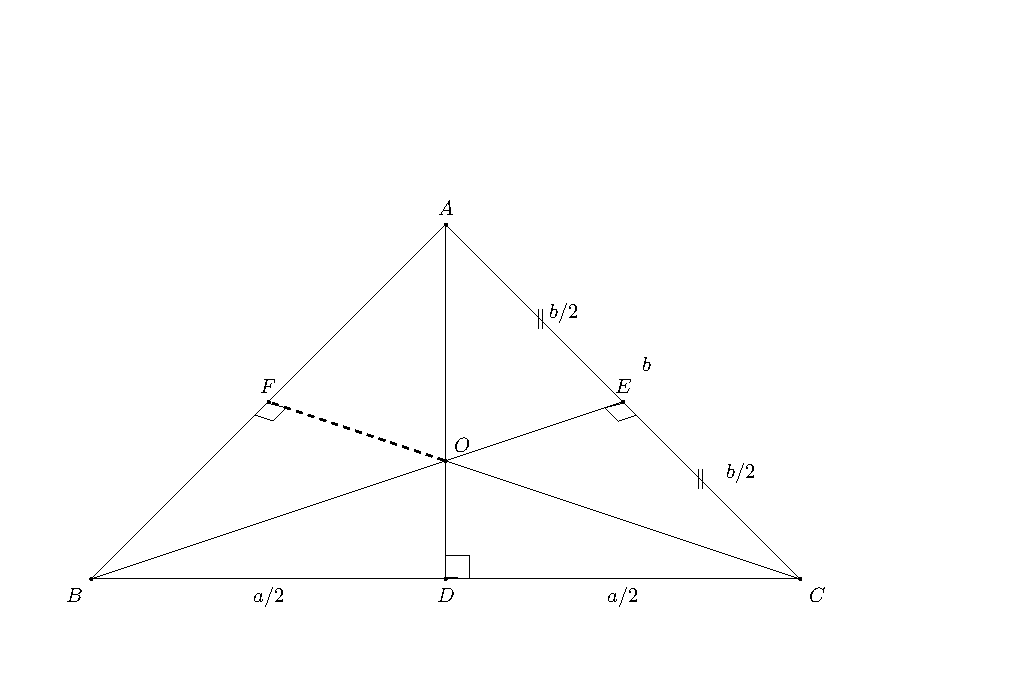
\includegraphics[width=\columnwidth]{./figs/fig_3.8.eps}
%		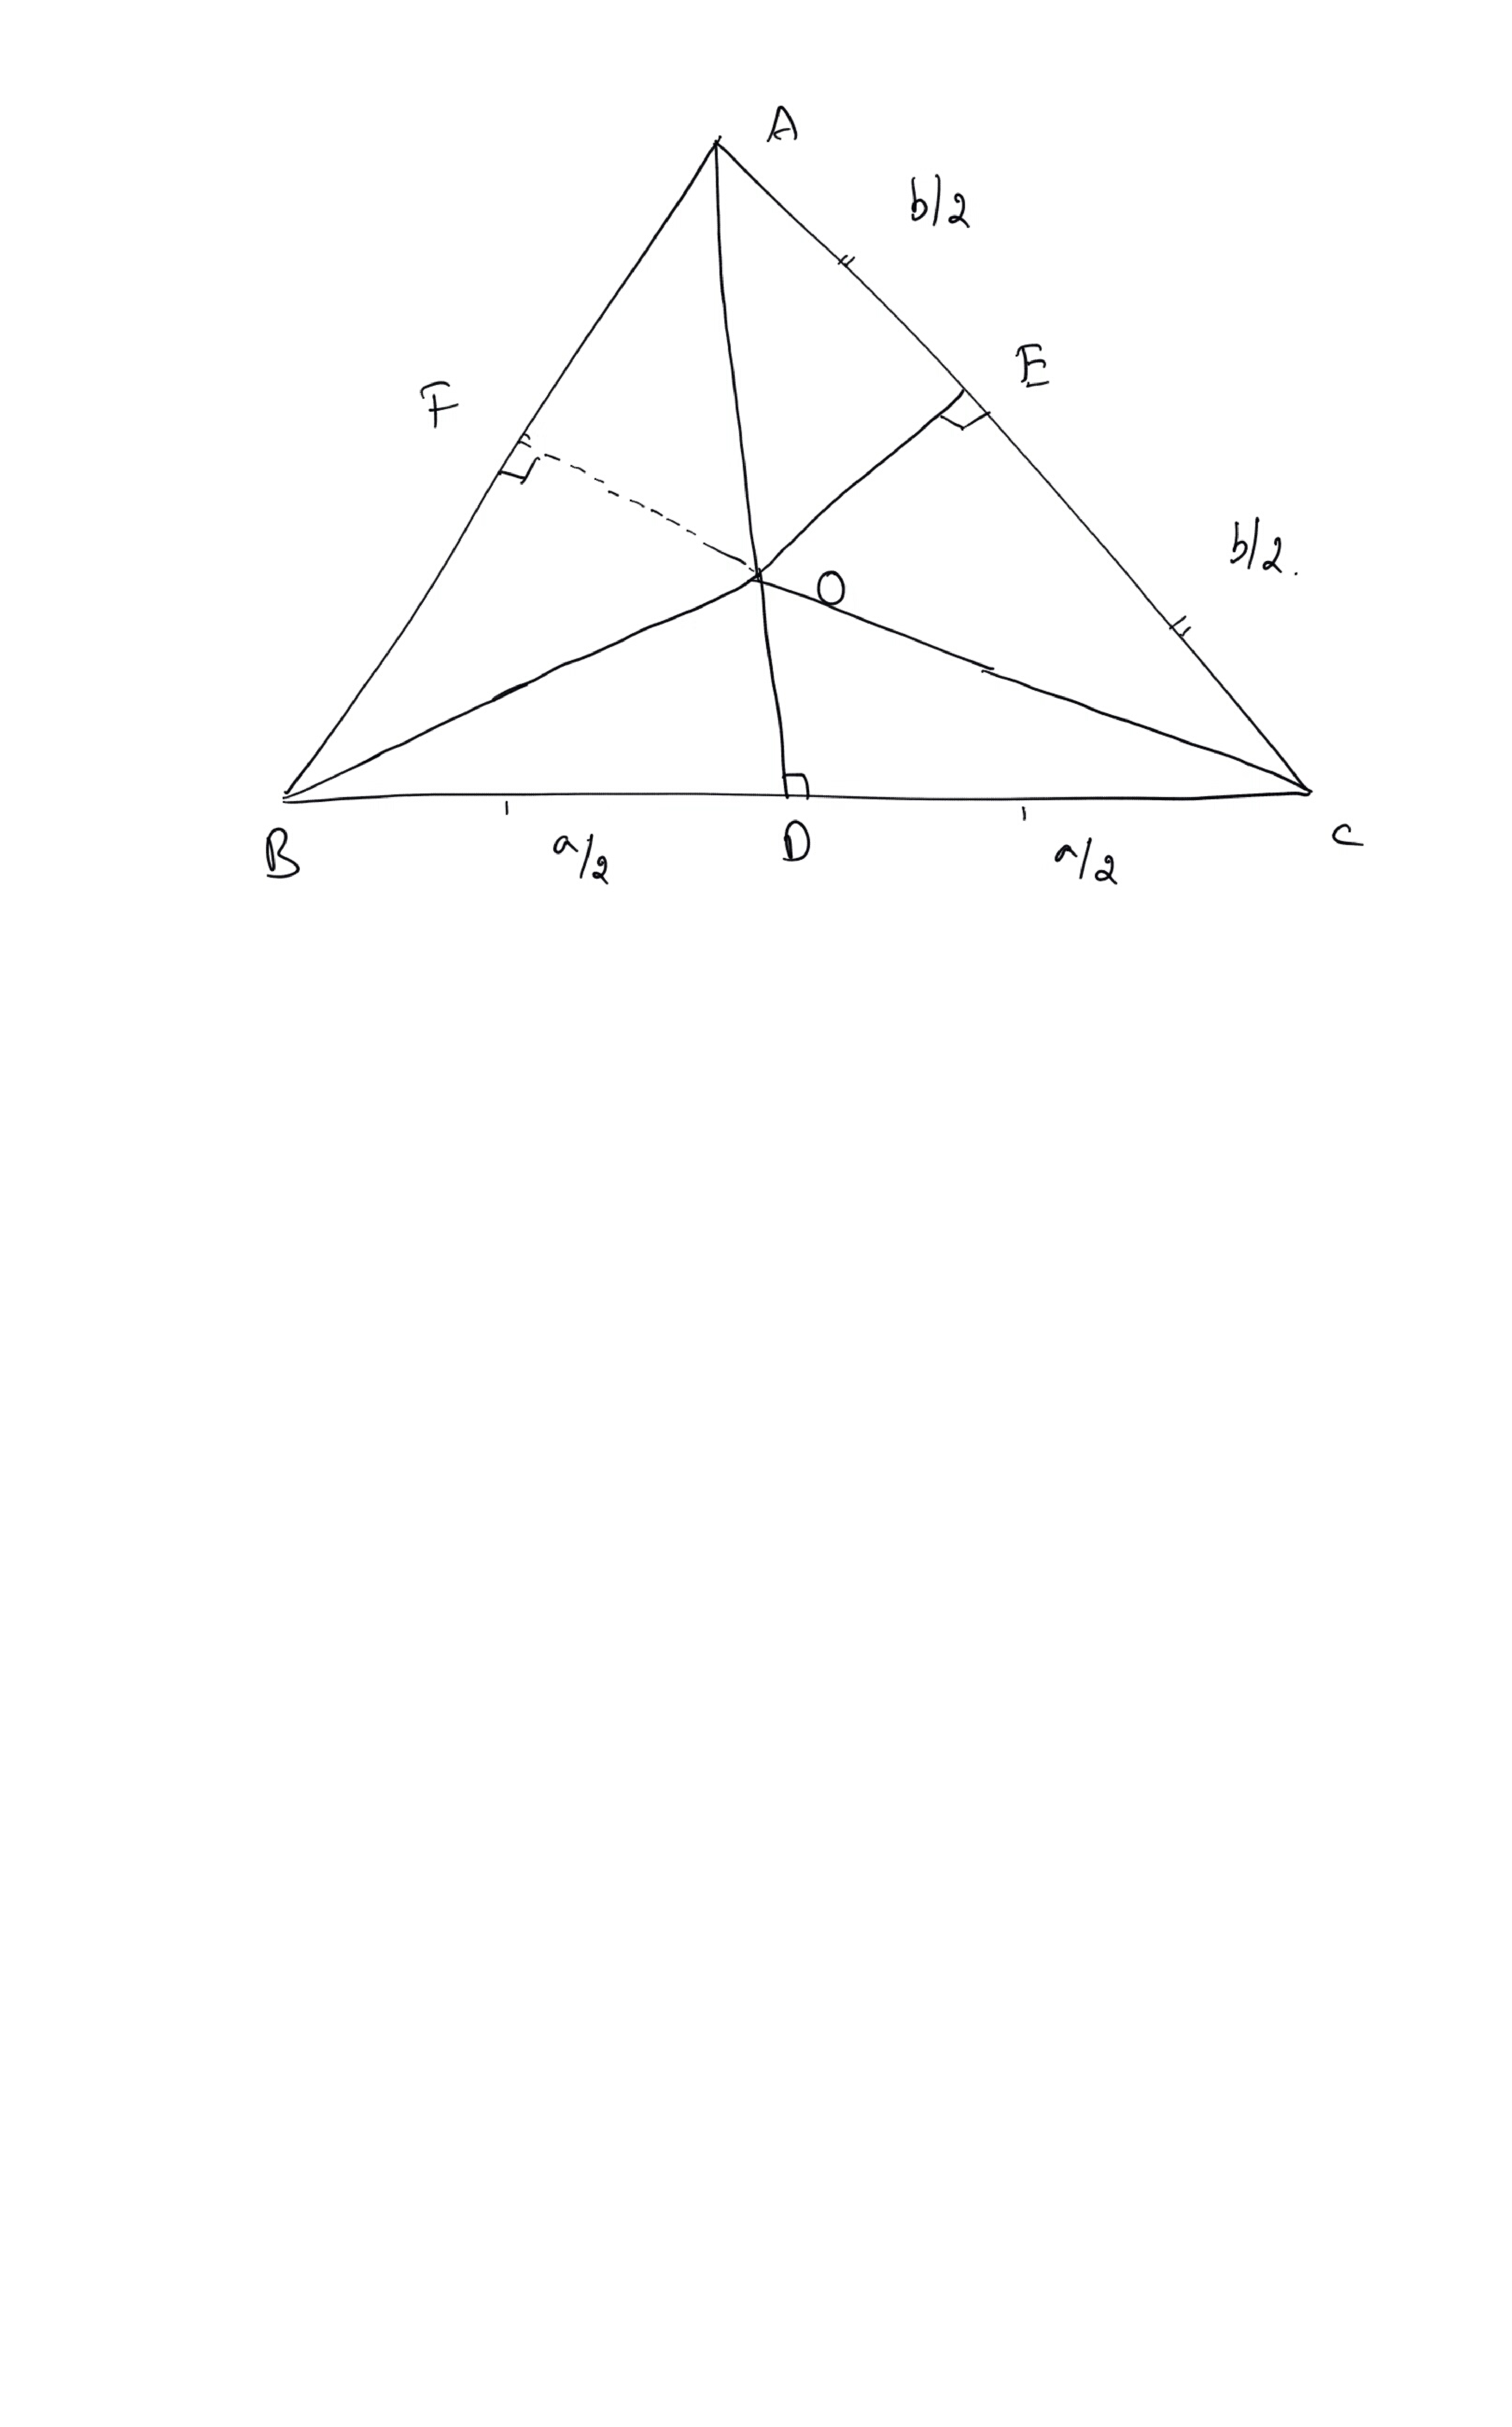
\includegraphics[width=\columnwidth]{./figs/ch3_perp_bisector}
		%\vspace*{-10cm}
%		\resizebox{\columnwidth}{!}{\documentclass{standalone}
\usepackage{tikz}
\usepackage{tkz-euclide}
\usetkzobj{all}
%\usepackage{amsmath}
\providecommand{\brak}[1]{\ensuremath{\left(#1\right)}}

\begin{document}
\begin{tikzpicture}
[scale=2,>=stealth,point/.style={draw,circle,fill = black,inner sep=0.5pt},]

\node (E) at (1.5, 1.5)[point,label=above :$E$] {};
\node (F) at (-1.5, 1.5)[point,label=above :$F$] {};
\node (A) at (0, 3)[point,label=above :$A$]{};
\node (B) at (-3, 0)[point,label=below left:$B$]{};
\node (C) at (3, 0)[point,label=below right:$C$]{};
\node (D) at (0,0)[point,label=below :$D$] {};
\node (O) at (0,1)[point,label=above right :$O$] {};


\draw (B)--(A);
\draw (A)--(C);
\draw (B)--(C);
\draw (B)--(E);
\draw (C)--(O);
\draw (A)--(D);
\draw [thick,dashed] (O) -- (F);

\node [above] at (1.7,1.7) {$b$};
\node [above] at (2.5,.75) {$b/2$};
\node [above] at (1,2.1) {$b/2$};
\node [above] at (-1.5,-0.3){$a/2$};
\node [above] at (1.5,-0.3){$a/2$};
\tkzMarkRightAngle[size=.16](B,F,O)
\tkzMarkRightAngle[size=.16](C,E,O)
\tkzMarkRightAngle[size=.2](A,D,C)
\draw   -- (4.3,1.7) node[midway] {$\parallel$};
\draw   -- (1.6,4.4) node[midway] {$\parallel$};

\end{tikzpicture}
\end{document}}
	\end{center}
	\caption{Perpendicular bisectors meet at a point}
	\label{ch3_perp_bisector}	
\end{figure}
%
\proof In $\Delta$s $ODB$ and $ODC$, using Budhayana's theorem,
%
\begin{equation}
\begin{split}
OB^2 &= OD^2 + BD^2 \\
OC^2 &= OD^2 + DC^2 
\end{split}
\end{equation}
%
Since $BD = DC = \frac{a}{2}$, $OB = OC$.  Similarly, it can be shown that $OA = OC$.  Thus, $OA=OB=OC$.
%
\begin{definition}
	In $\Delta AOB$, $OA = OB$.  Such a triangle is known as an isoceles triangle.
\end{definition}
%
\begin{problem}
	Show that $AF = BF$.
\end{problem}
\proof Trivial using Budhayana's theorem.  This shows that $OF$ is a perpendicular bisector of $AB$. 
{\em Conclusion:}  The perpendicular bisectors of a triangle meet at a point.
%
\subsection{Perpendiculars from Vertex to Opposite Side}
	%
	%
	In Fig. \ref{ch3_perp_triang}, $AD \perp BC$ and $BE \perp AC$. $CF$ passes through $O$ and meets
	$AB$ at $F$.  	
\begin{problem}
	Show that 
	\begin{align}
	OE = c \cos A \cot C
	\end{align}
\end{problem}
	\begin{figure}[!h]
		\begin{center}
			
			%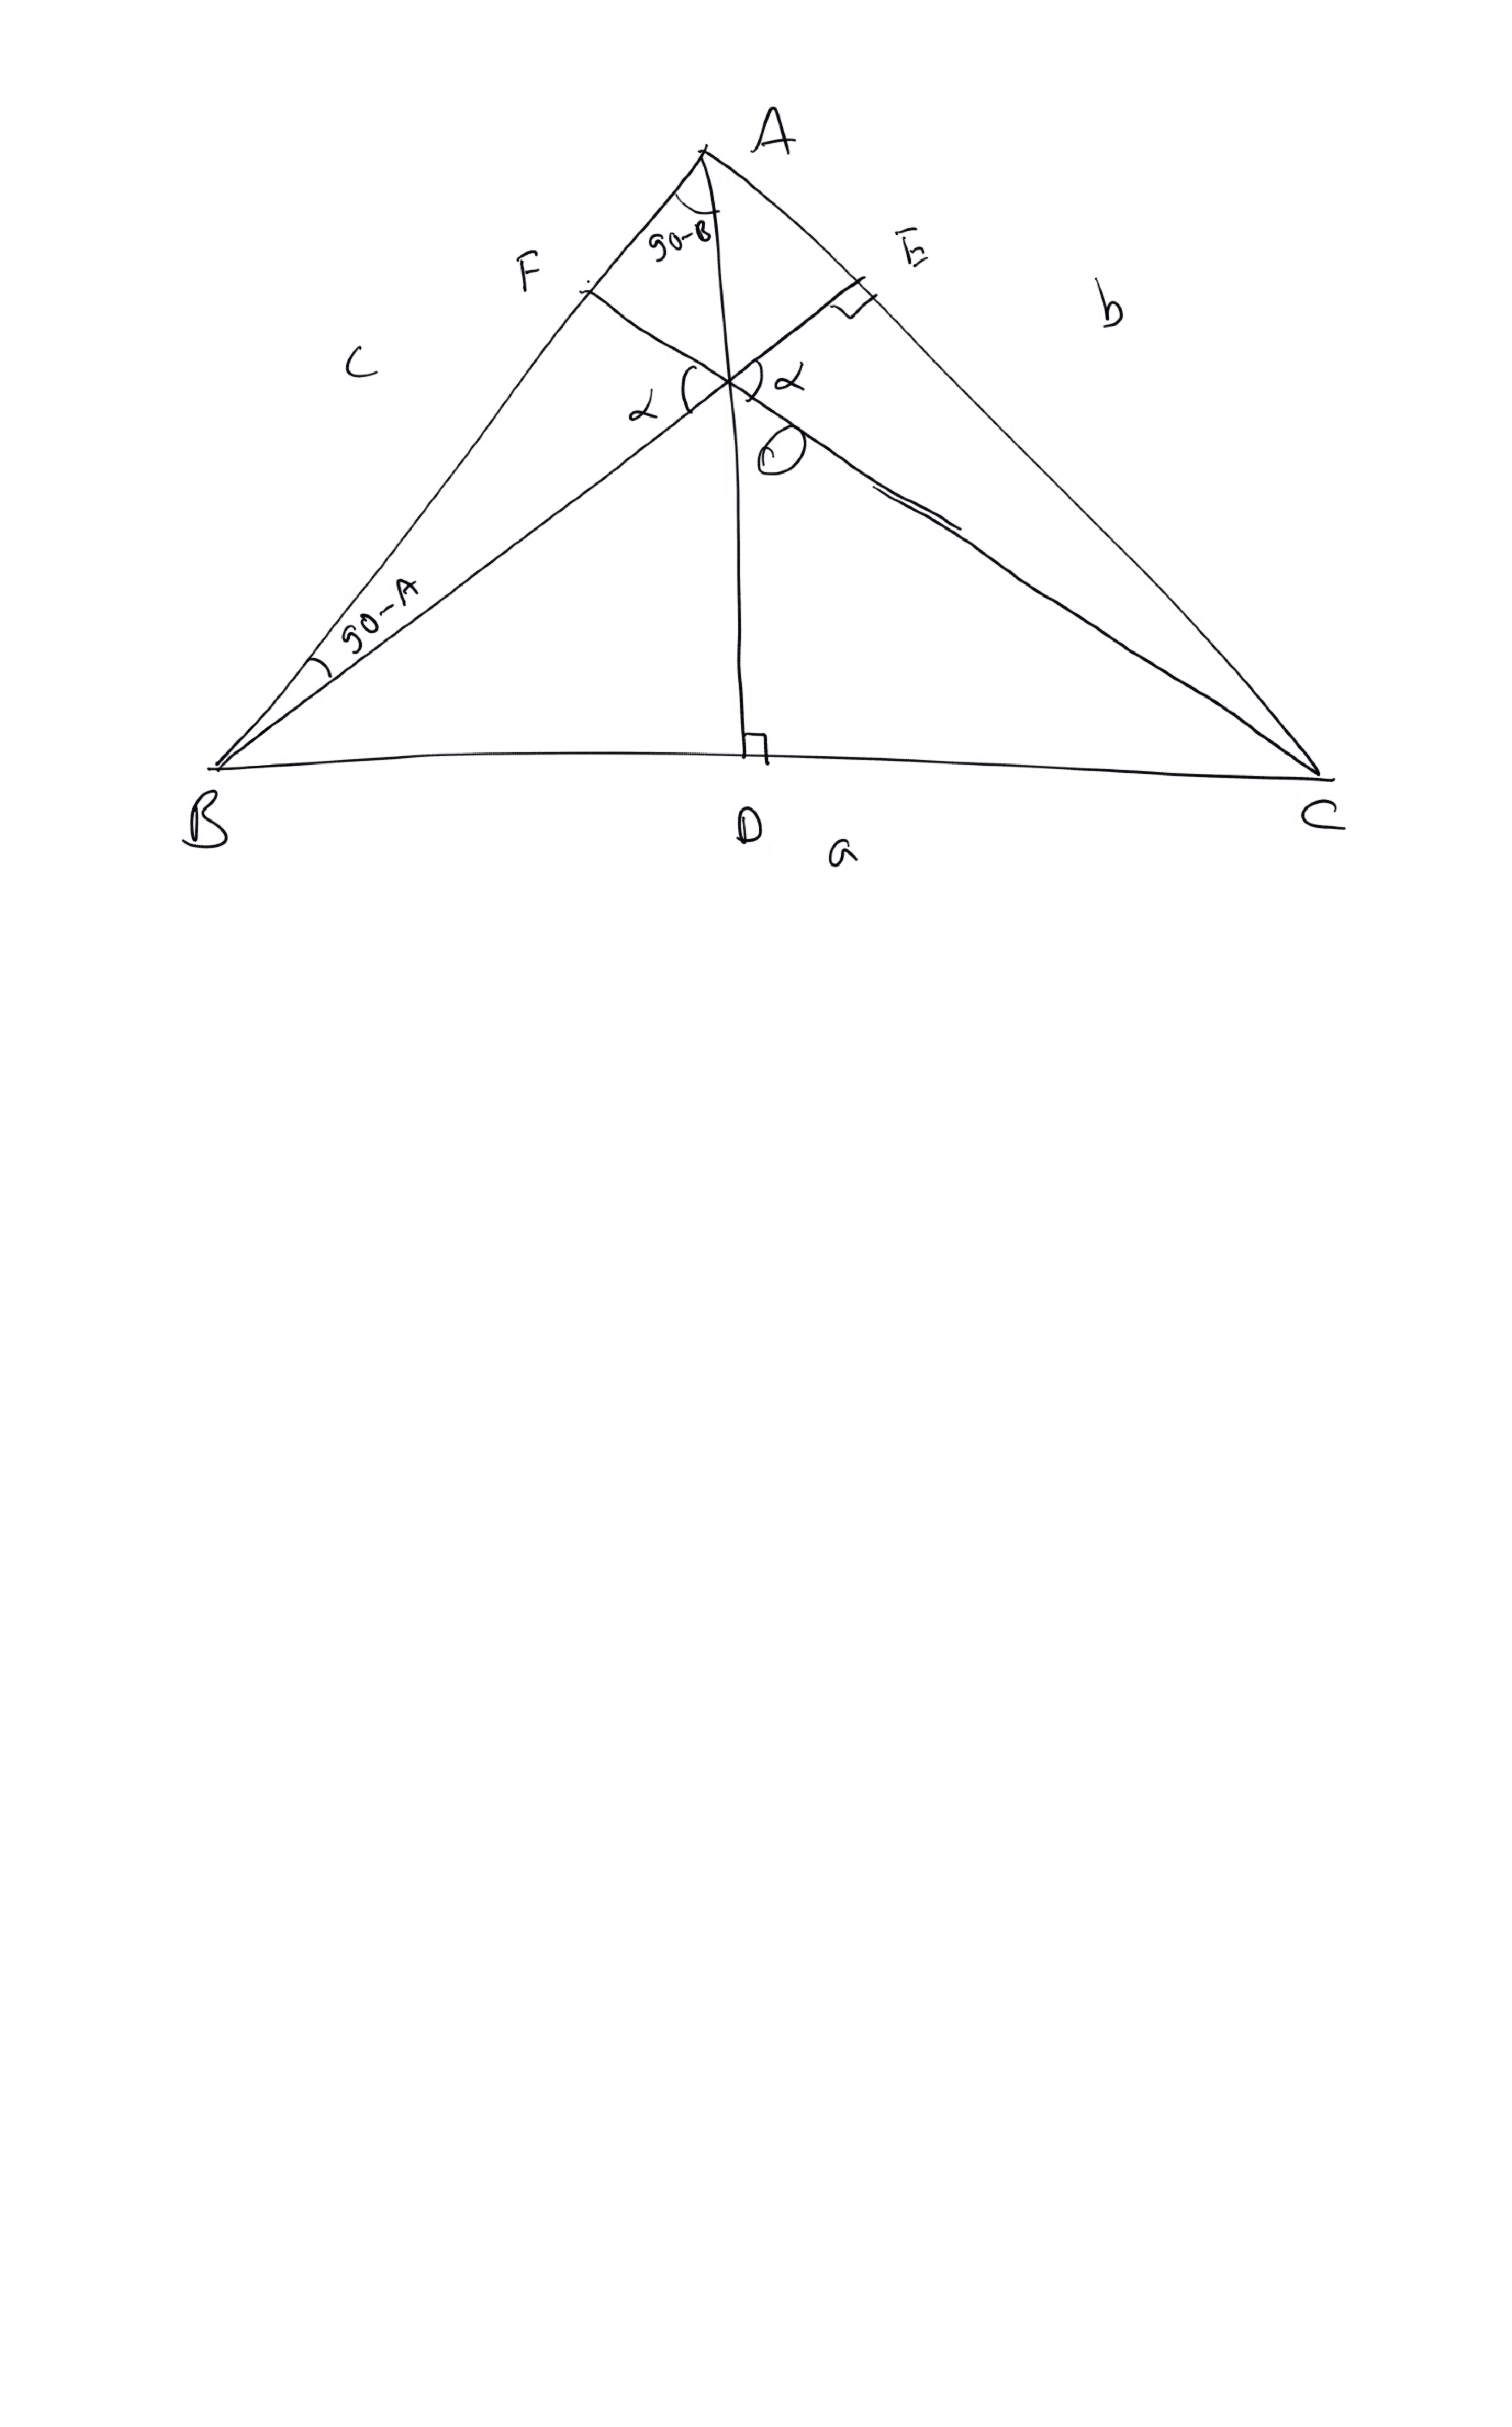
\includegraphics[width=\columnwidth]{./figs/ch3_perp_triang}
			%\vspace*{-10cm}
			\resizebox{\columnwidth}{!}{\begin{tikzpicture}
[scale=2,>=stealth,point/.style={draw,circle,fill = black,inner sep=0.5pt},]

\node (E) at (1.5, 1.5)[point,label=above :$E$] {};
\node (F) at (-1.5, 1.5)[point,label=above :$F$] {};
\node (A) at (0, 3)[point,label=above :$A$]{};
\node (B) at (-3, 0)[point,label=below left:$B$]{};
\node (C) at (3, 0)[point,label=below right:$C$]{};
\node (O) at (0,1)[point,label=above right :$O$] {};
\node (D) at (0,0)[point,label=below :$D$] {};


\draw (B)--(A);
\draw (A)--(C);
\draw (B)--(E);
\draw (C)--(F);
\draw (B)--(C);
\draw (A)--(D);

\node [below] at (0,-0.3) {$a$};
\node [above] at (-1.7,1.7) {$c$};
\node [above] at (1.7,1.7) {$b$};
\node [above] at (1,1.3) {$p$};
\node [above] at (-1,1.3) {$q$};
\node [above] at (-2.3,0.24){\rotatebox{45}{$90-A$}};
\node [above] at (-0.4,2.1) {\rotatebox{45}{$90-B$}};
\node [above] at (0.4,2.1) {\rotatebox{-45}{$90-C$}};

\tkzMarkAngle[size=.3](F,O,B);
\tkzMarkAngle[size=.3](C,O,E);
\tkzMarkAngle[size=.4](O,B,F);
\tkzMarkAngle[size=.2](F,A,O);
\tkzMarkAngle[size=.3](O,A,E);
\draw (-0.5,1) node{$\alpha$};
\draw (0.5,1) node{$\alpha$};

\end{tikzpicture}
}
		\end{center}
		\caption{Perpendiculars from vertex to opposite side meet at a point}
		\label{ch3_perp_triang}	
	\end{figure}
%
\proof In $\Delta$ s $AEB$ and $AEO$,
%
\begin{align}
AE &= c \cos A \\
OE &= AE \tan \brak{90^{\degree} - C} \brak{\because ADC \text{ is right angled}} \\
&= AE \cot C
\end{align}
%
From both the above, we get the desired result.
%
\begin{problem}
	Show that $\alpha = A$.
\end{problem}
\proof In $\Delta OEC$,
%
\begin{equation}
CE = a \cos C \brak{\because BEC \text{ is right angled}}
\end{equation}
%
Hence,
%
\begin{equation}
\begin{split}
\tan \alpha &= \frac{CE}{OE} \\
&=  \frac{a \cos C}{c \cos A \cot C} \\
&=  \frac{a \cos C \sin C}{c \cos A \cos C} \\
&= \frac{a \sin C}{c \cos A } \\
&= \frac{c \sin A}{c \cos A } \brak{\because \frac{a}{\sin A} = \frac{c}{\sin C}}\\
&= \tan A\\
\Rightarrow \alpha = A
\end{split}
\end{equation}
%
\begin{problem}
	Show that $CF \perp AB$
\end{problem}
\proof Consider triangle OFB and the result of the previous problem.  $\because$ the sum of the angles of a triangle is $180^{\degree}$, $\angle CFB = 90^{\degree}$.
{\em Conclusion: The perperdiculars from the vertex of a triangle to the opposite side meet at a point.}
%%
%%%\newpage
%\section{The Circle}
%\subsection{Angle Bisectors}

\begin{figure}[!h]
	\begin{center}
		
		%
\includegraphics[width=\columnwidth]{./figs/ch3_angle_bisector}
		%\vspace*{-10cm}
		\resizebox{\columnwidth}{!}{\begin{tikzpicture}
[scale=2,>=stealth,point/.style={draw,circle,fill = black,inner sep=0.5pt},]

\node (D) at (0, 0)[point,label=below :$D$] {};
\node (A) at (0, 3)[point,label=above :$A$]{};
\node (B) at (-3, 0)[point,label=below left:$B$]{};
\node (C) at (3, 0)[point,label=below right:$C$]{};
\node (O) at (0, 1.3)[point,label=below right:$O$]{};
\node (F) at (-1.1, 1.9)[point,label=above left:$F$]{};
\node (E) at (1.1, 1.9)[point,label=above right:$E$]{};

\draw (D)--(B);
\draw (B)--(A);
\draw (A)--(C);
\draw (C)--(D);
\draw [thick,dashed] (A) -- (D);
\draw [thick,dashed] (O) -- (E);
\draw [thick,dashed] (O) -- (F);
\draw (B)--(O);
\draw (C)--(O);

\tkzMarkRightAngle[size=.2](A,D,C)
\tkzMarkRightAngle[size=.15](B,F,O);
\tkzMarkRightAngle[size=.15](C,E,O);
\tkzMarkAngle[size=.4](D,B,O);
\tkzMarkAngle[size=.35](O,B,F);
\tkzMarkAngle[size=.54](E,C,O);
\tkzMarkAngle[size=.5](E,C,O);
\tkzMarkAngle[size=.6](O,C,D);
\tkzMarkAngle[size=.65](O,C,D);

\end{tikzpicture}}
	\end{center}
	\caption{Angle bisectors meet at a point}
	\label{ch3_angle_bisector}	
\end{figure}

\begin{definition}
	In Fig. \ref{ch3_angle_bisector}, $OB$ divides the  $\angle B$ into half, i.e.\begin{equation}
	\angle OBC = \angle OBA
	\end{equation}
	$OB$ is known as an angle bisector.
\end{definition}
	$OB$ and $OC$ are angle bisectors of angles $B$ and $C$. $OA$ is joined and $OD, OF$ and $OE$ are perpendiculars to sides $a,b$ and $c$.
\begin{problem}
  Show that $OD = OE = OF$.
\end{problem}
\proof In $\Delta$s $ODC$ and $OEC$,
\begin{align}
OD &= OC \sin \frac{C}{2}
\\
OE &= OC \sin \frac{C}{2} 
\\
\Rightarrow OD &=OE.
\end{align}
Similarly,
\begin{equation}
OD = OF.
\end{equation}
%
\begin{problem}
	Show that OA is the angle bisector of $\angle A$
\end{problem}
\proof In $\Delta$s $OFA$ and $OEA$,
\begin{align}
OF &= OE
\\
\Rightarrow OA \sin OAF &= OA \sin OAE \\
\Rightarrow \sin OAF &=  \sin OAE \\
\Rightarrow \angle OAF &= \angle OAE
\end{align}
which proves that $OA$ bisects $\angle A$.
{\em Conclusion:} The angle bisectors of a triangle meet at a point.


\subsection{Congruent Triangles}
%
\begin{problem}
	Show that in $\Delta$s $ODC$ and $OEC$, corresponding sides and angles are equal.
\end{problem}
\begin{definition}
	Note that    $\Delta$s $ODC$ and $OEC$ are known as congruent triangles.  To show that two triangles are congruent, it is sufficient to show that some angles and sides are equal.
\end{definition}
\begin{problem}
SSS:	Show that if the corresponding sides of three triangles are equal, the triangles are congruent.
\end{problem}
\begin{problem}
ASA:	Show that if two angles and any one side  are equal in corresponding triangles, the triangles are congruent.
\end{problem}
\begin{problem}
SAS:	Show that if two sides and the angle between them are equal in corresponding triangles, the triangles are congruent.
\end{problem}
\begin{problem}
RHS:	For two right angled triangles, if the hypotenuse and one of the sides are equal, show that the triangles are congruent.
\end{problem}
	%
%%
\subsection{Perpendicular Bisectors}
\begin{definition}
	In Fig. \ref{ch3_perp_bisector}, OD $\perp BC$ and $BD=DC$. $OD$ is defined as the perpendicular bisector of $BC$.
\end{definition}

\begin{problem}
	In Fig. \ref{ch3_perp_bisector}, show that $OA=OB=OC$.
\end{problem}
%%
%%
\begin{figure}[!h]
	\begin{center}
		
		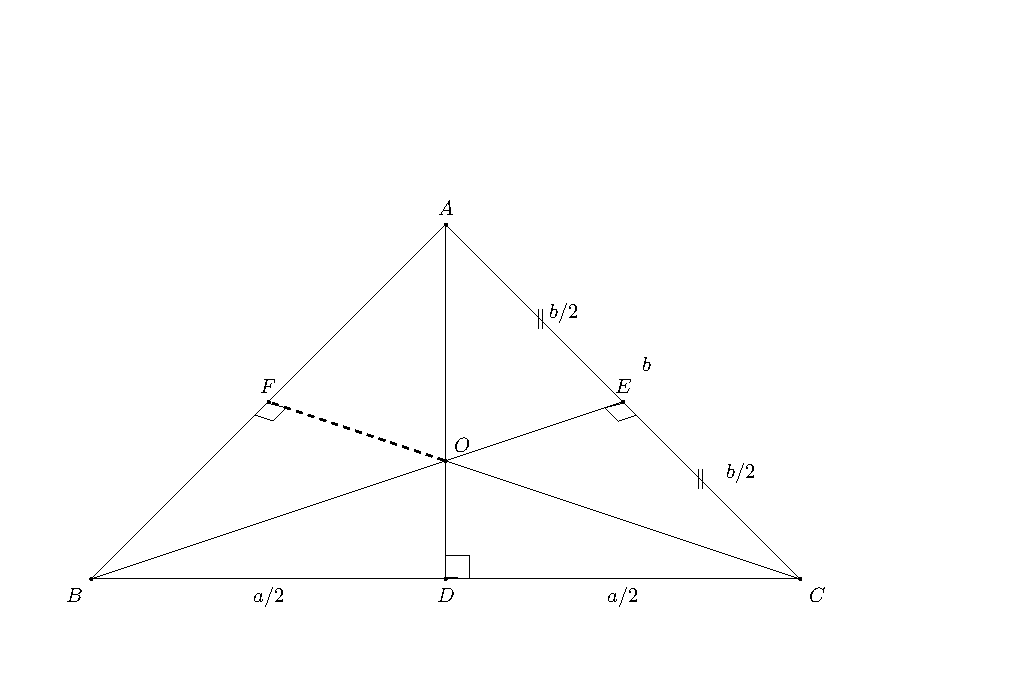
\includegraphics[width=\columnwidth]{./figs/fig_3.8.eps}
%		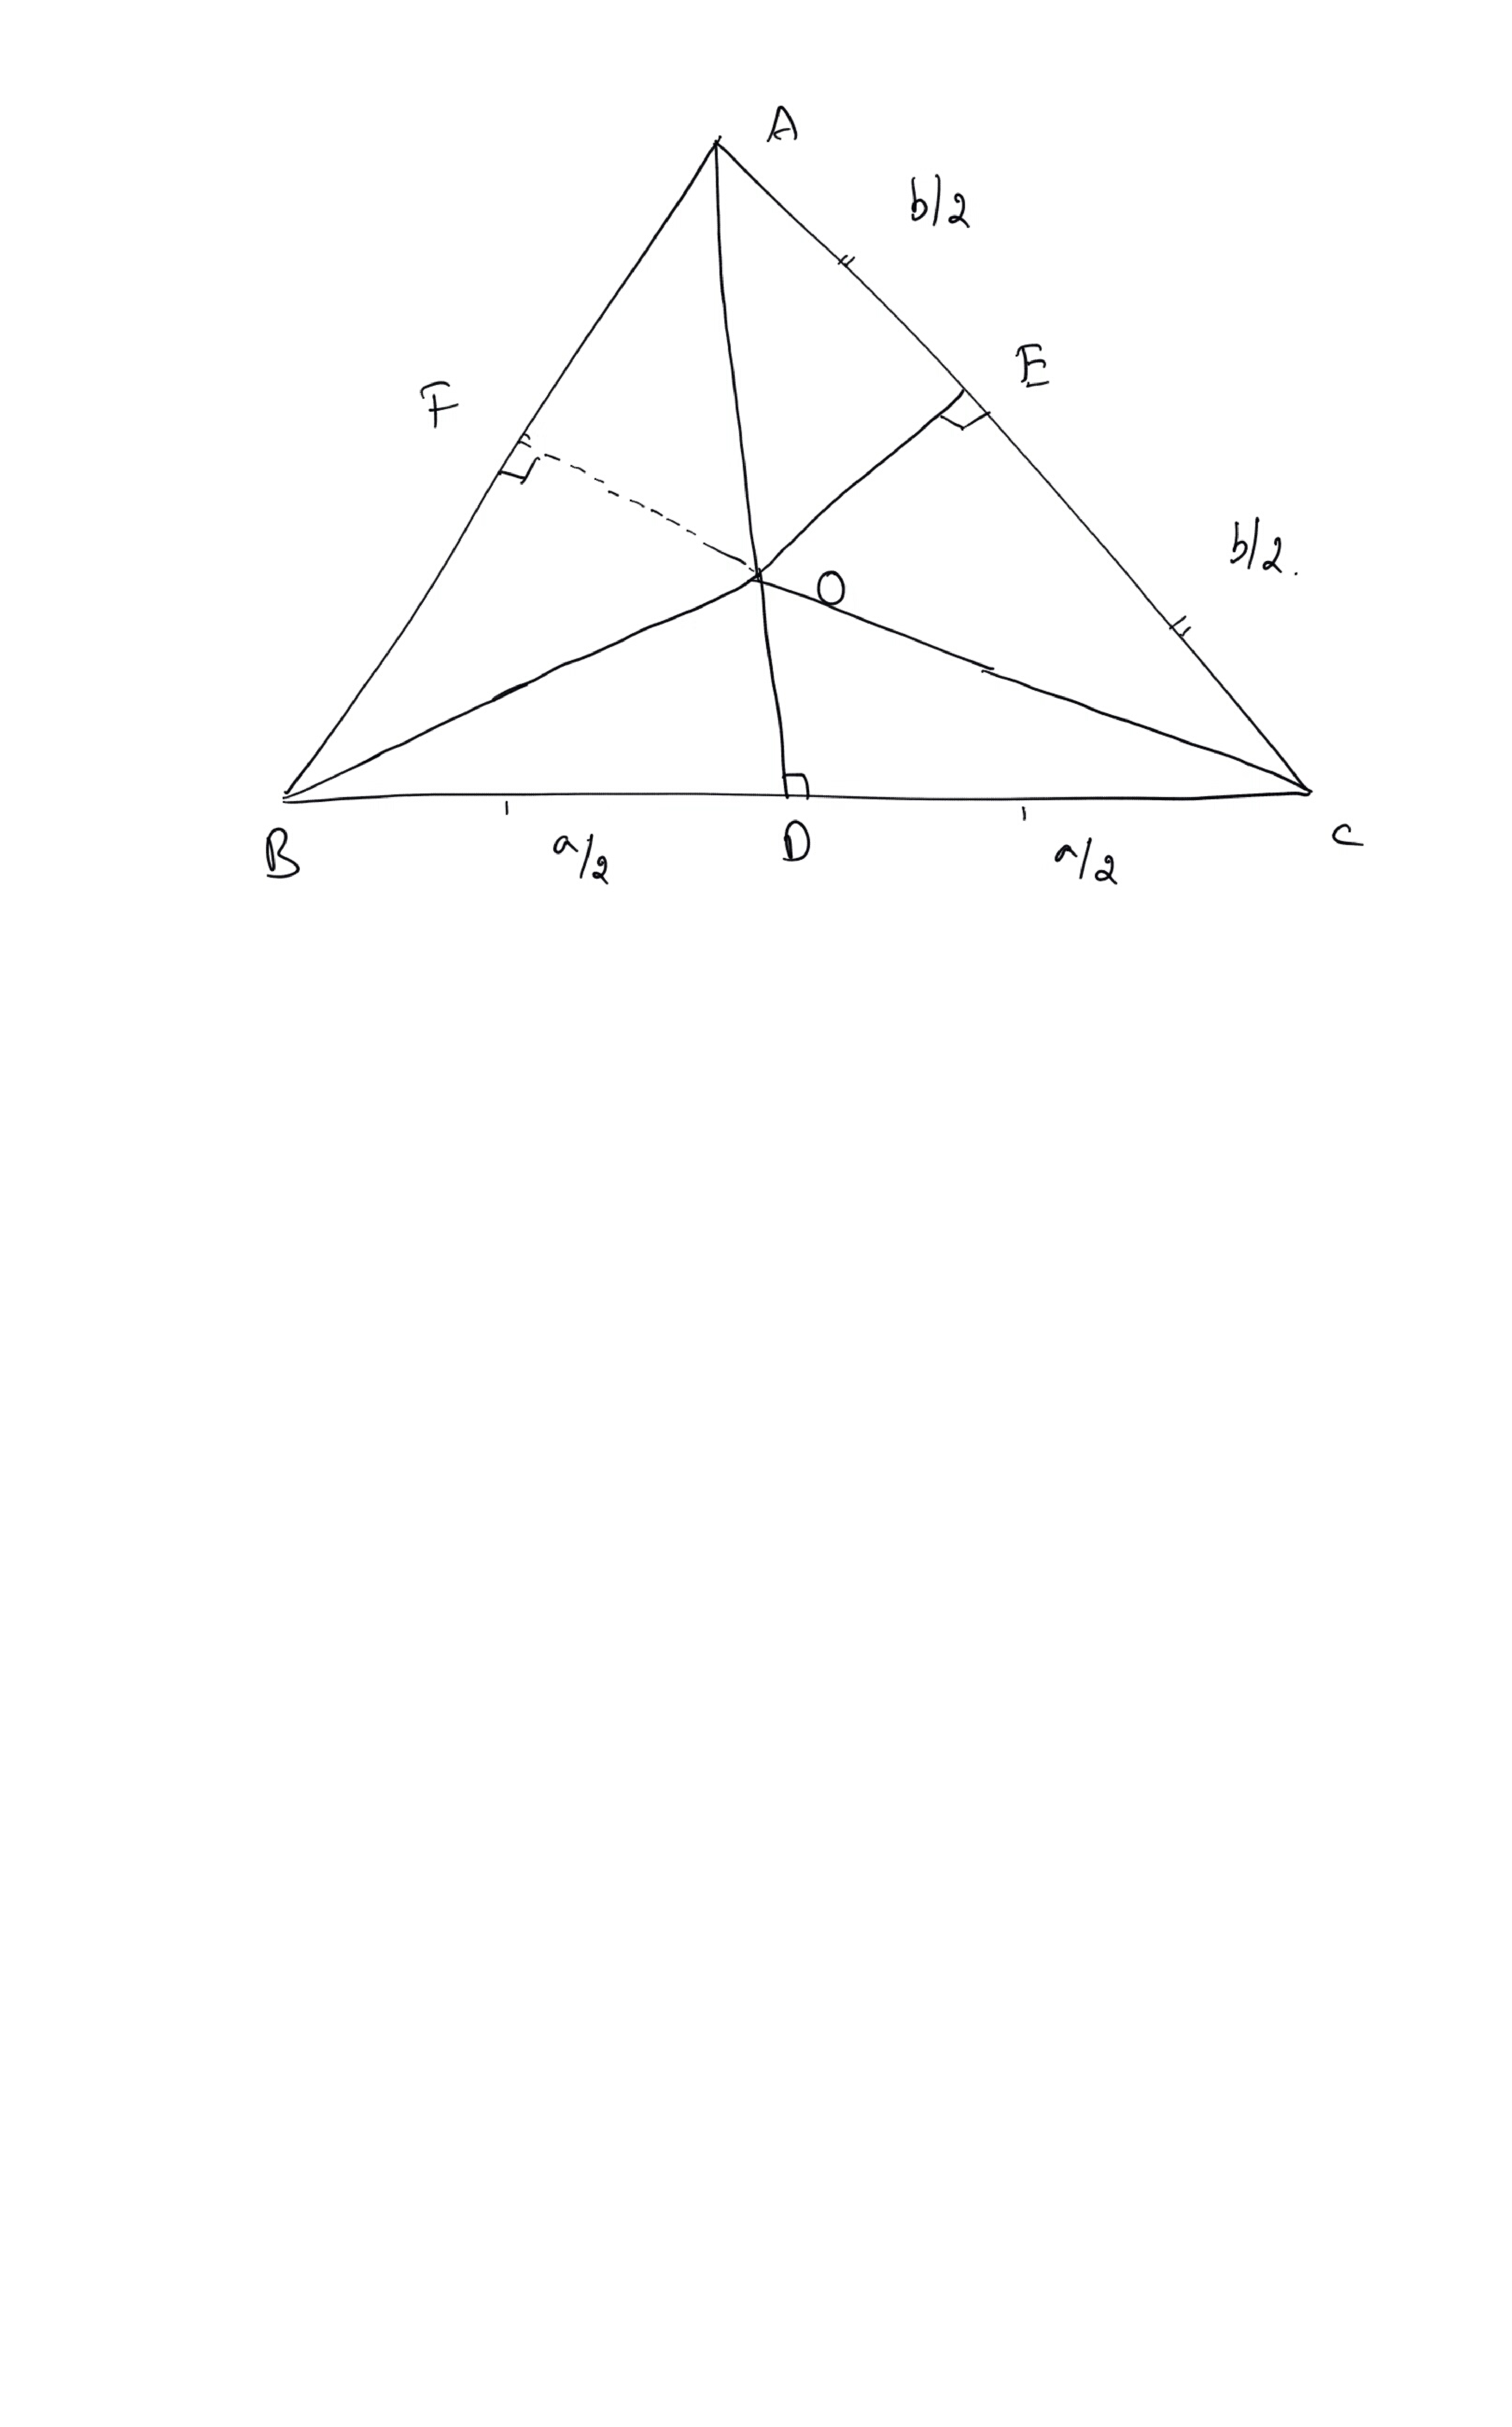
\includegraphics[width=\columnwidth]{./figs/ch3_perp_bisector}
		%\vspace*{-10cm}
%		\resizebox{\columnwidth}{!}{\documentclass{standalone}
\usepackage{tikz}
\usepackage{tkz-euclide}
\usetkzobj{all}
%\usepackage{amsmath}
\providecommand{\brak}[1]{\ensuremath{\left(#1\right)}}

\begin{document}
\begin{tikzpicture}
[scale=2,>=stealth,point/.style={draw,circle,fill = black,inner sep=0.5pt},]

\node (E) at (1.5, 1.5)[point,label=above :$E$] {};
\node (F) at (-1.5, 1.5)[point,label=above :$F$] {};
\node (A) at (0, 3)[point,label=above :$A$]{};
\node (B) at (-3, 0)[point,label=below left:$B$]{};
\node (C) at (3, 0)[point,label=below right:$C$]{};
\node (D) at (0,0)[point,label=below :$D$] {};
\node (O) at (0,1)[point,label=above right :$O$] {};


\draw (B)--(A);
\draw (A)--(C);
\draw (B)--(C);
\draw (B)--(E);
\draw (C)--(O);
\draw (A)--(D);
\draw [thick,dashed] (O) -- (F);

\node [above] at (1.7,1.7) {$b$};
\node [above] at (2.5,.75) {$b/2$};
\node [above] at (1,2.1) {$b/2$};
\node [above] at (-1.5,-0.3){$a/2$};
\node [above] at (1.5,-0.3){$a/2$};
\tkzMarkRightAngle[size=.16](B,F,O)
\tkzMarkRightAngle[size=.16](C,E,O)
\tkzMarkRightAngle[size=.2](A,D,C)
\draw   -- (4.3,1.7) node[midway] {$\parallel$};
\draw   -- (1.6,4.4) node[midway] {$\parallel$};

\end{tikzpicture}
\end{document}}
	\end{center}
	\caption{Perpendicular bisectors meet at a point}
	\label{ch3_perp_bisector}	
\end{figure}
%
\proof In $\Delta$s $ODB$ and $ODC$, using Budhayana's theorem,
%
\begin{equation}
\begin{split}
OB^2 &= OD^2 + BD^2 \\
OC^2 &= OD^2 + DC^2 
\end{split}
\end{equation}
%
Since $BD = DC = \frac{a}{2}$, $OB = OC$.  Similarly, it can be shown that $OA = OC$.  Thus, $OA=OB=OC$.
%
\begin{definition}
	In $\Delta AOB$, $OA = OB$.  Such a triangle is known as an isoceles triangle.
\end{definition}
%
\begin{problem}
	Show that $AF = BF$.
\end{problem}
\proof Trivial using Budhayana's theorem.  This shows that $OF$ is a perpendicular bisector of $AB$. 
{\em Conclusion:}  The perpendicular bisectors of a triangle meet at a point.
%
\subsection{Perpendiculars from Vertex to Opposite Side}
	%
	%
	In Fig. \ref{ch3_perp_triang}, $AD \perp BC$ and $BE \perp AC$. $CF$ passes through $O$ and meets
	$AB$ at $F$.  	
\begin{problem}
	Show that 
	\begin{align}
	OE = c \cos A \cot C
	\end{align}
\end{problem}
	\begin{figure}[!h]
		\begin{center}
			
			%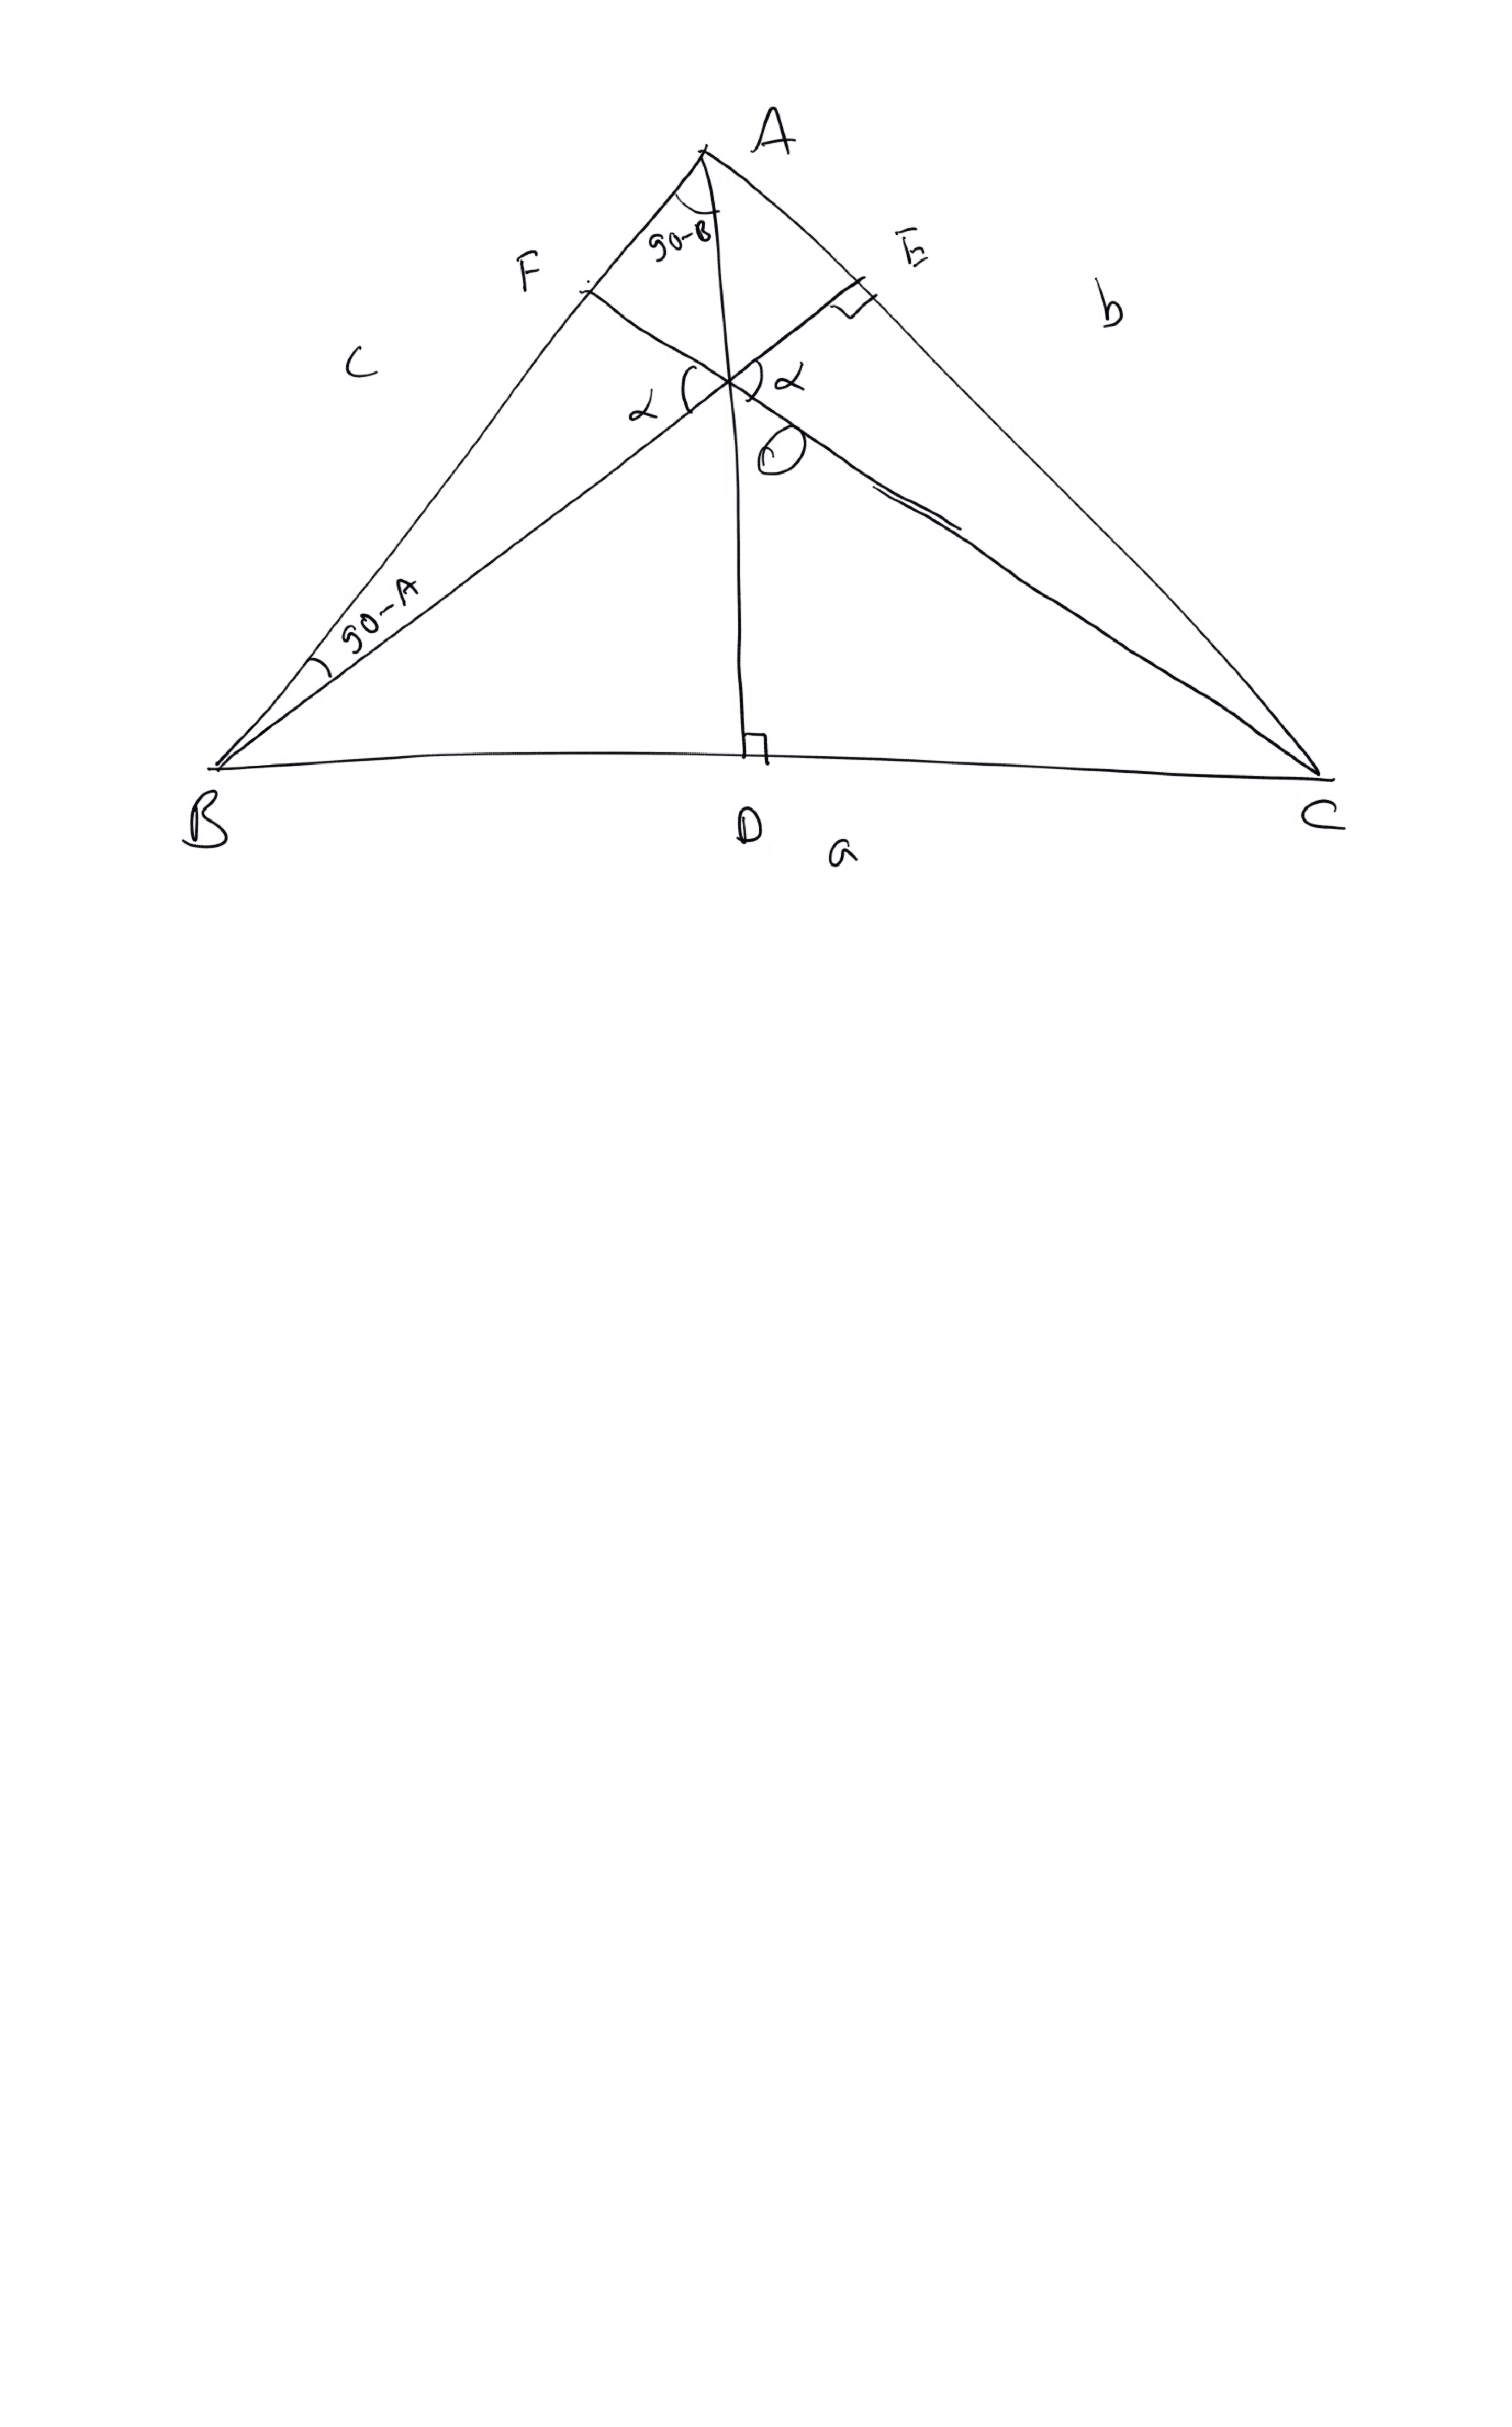
\includegraphics[width=\columnwidth]{./figs/ch3_perp_triang}
			%\vspace*{-10cm}
			\resizebox{\columnwidth}{!}{\begin{tikzpicture}
[scale=2,>=stealth,point/.style={draw,circle,fill = black,inner sep=0.5pt},]

\node (E) at (1.5, 1.5)[point,label=above :$E$] {};
\node (F) at (-1.5, 1.5)[point,label=above :$F$] {};
\node (A) at (0, 3)[point,label=above :$A$]{};
\node (B) at (-3, 0)[point,label=below left:$B$]{};
\node (C) at (3, 0)[point,label=below right:$C$]{};
\node (O) at (0,1)[point,label=above right :$O$] {};
\node (D) at (0,0)[point,label=below :$D$] {};


\draw (B)--(A);
\draw (A)--(C);
\draw (B)--(E);
\draw (C)--(F);
\draw (B)--(C);
\draw (A)--(D);

\node [below] at (0,-0.3) {$a$};
\node [above] at (-1.7,1.7) {$c$};
\node [above] at (1.7,1.7) {$b$};
\node [above] at (1,1.3) {$p$};
\node [above] at (-1,1.3) {$q$};
\node [above] at (-2.3,0.24){\rotatebox{45}{$90-A$}};
\node [above] at (-0.4,2.1) {\rotatebox{45}{$90-B$}};
\node [above] at (0.4,2.1) {\rotatebox{-45}{$90-C$}};

\tkzMarkAngle[size=.3](F,O,B);
\tkzMarkAngle[size=.3](C,O,E);
\tkzMarkAngle[size=.4](O,B,F);
\tkzMarkAngle[size=.2](F,A,O);
\tkzMarkAngle[size=.3](O,A,E);
\draw (-0.5,1) node{$\alpha$};
\draw (0.5,1) node{$\alpha$};

\end{tikzpicture}
}
		\end{center}
		\caption{Perpendiculars from vertex to opposite side meet at a point}
		\label{ch3_perp_triang}	
	\end{figure}
%
\proof In $\Delta$ s $AEB$ and $AEO$,
%
\begin{align}
AE &= c \cos A \\
OE &= AE \tan \brak{90^{\degree} - C} \brak{\because ADC \text{ is right angled}} \\
&= AE \cot C
\end{align}
%
From both the above, we get the desired result.
%
\begin{problem}
	Show that $\alpha = A$.
\end{problem}
\proof In $\Delta OEC$,
%
\begin{equation}
CE = a \cos C \brak{\because BEC \text{ is right angled}}
\end{equation}
%
Hence,
%
\begin{equation}
\begin{split}
\tan \alpha &= \frac{CE}{OE} \\
&=  \frac{a \cos C}{c \cos A \cot C} \\
&=  \frac{a \cos C \sin C}{c \cos A \cos C} \\
&= \frac{a \sin C}{c \cos A } \\
&= \frac{c \sin A}{c \cos A } \brak{\because \frac{a}{\sin A} = \frac{c}{\sin C}}\\
&= \tan A\\
\Rightarrow \alpha = A
\end{split}
\end{equation}
%
\begin{problem}
	Show that $CF \perp AB$
\end{problem}
\proof Consider triangle OFB and the result of the previous problem.  $\because$ the sum of the angles of a triangle is $180^{\degree}$, $\angle CFB = 90^{\degree}$.
{\em Conclusion: The perperdiculars from the vertex of a triangle to the opposite side meet at a point.}
%
%\section{Circle}
%\subsection{Chord of a Circle}

\begin{figure}[!h]
	\begin{center}
		
		
\includegraphics[width=\columnwidth]{./figs/ch4_circle_def}
		\vspace*{-10cm}
	\end{center}
	\caption{Circle Definitions}
	\label{ch4_circle_def}	
\end{figure}
\begin{definition}
	Fig. \ref{ch4_circle_def} represents a circle.  The points in the circle are at a distance $r$ from the centre $O$.  $r$ is known as the radius.
\end{definition}

\subsection{Chords of a circle}
\begin{definition}
	In Fig. \ref{ch4_circle_def}, $A$ and $B$ are points on the circle.  The line $AB$ is known as a chord of the circle.
\end{definition}
%
%
\begin{problem}
	\label{ch4_prob_circle_subtend}
	In Fig. \ref{ch4_circle_subtend}  Show that $\angle OAB = 2\angle APB $.
\end{problem}
\begin{figure}[!h]
	\begin{center}
		
		
\includegraphics[width=\columnwidth]{./figs/ch4_circle_subtend}
		\vspace*{-10cm}
	\end{center}
	\caption{Angle subtended by chord $AB$ at the centre $O$ is twice the angle subtended at $P$. }
	\label{ch4_circle_subtend}	
\end{figure}

\proof In Fig. \ref{ch4_circle_subtend}, the triangeles $OPA$ and $OPB$ are isosceles. Hence,
%
\begin{align}
\angle OPB = \angle OBP &= \theta_1 \\
\angle OPA = \angle OAP &= \theta_2
\end{align}
%
Also, $\alpha$ and $\beta$ are exterior angles corresponding to the triangle $OPB$ and $OPA$ respectively. Hence
%
\begin{align}
\alpha &= 2\theta_1 \\
\beta &= 2\theta_2
\end{align}
%
Thus,
%
\begin{align}
\angle AOB &= \alpha + \beta \\
&= \theta_1 + \theta_2 \\
&= \angle APB
\end{align}
%
\begin{definition}
	The diameter of a circle is the chord that divides the circle into two equal parts. In Fig. \ref{ch4_circle_dia}, $AB$ is the diameter and passes through the centre $O$
\end{definition}
%
\begin{problem}
In Fig. \ref{ch4_circle_dia}, show that $\angle APB = 90^{\degree}$ .
\end{problem}
%
\begin{figure}[!h]
	\begin{center}
		
		
\includegraphics[width=\columnwidth]{./figs/ch4_circle_dia}
		\vspace*{-10cm}
	\end{center}
	\caption{Diameter of a circle.}
	\label{ch4_circle_dia}	
\end{figure}

\begin{problem}
	In Fig. \ref{ch4_chord_product}, show that 
	\begin{equation}
	\begin{split}
\angle ABD &= \angle ACD \\
\angle CAB &= \angle CDB	
	\end{split}
	\end{equation}
\end{problem}
\begin{figure}[!h]
	\begin{center}
		
		
\includegraphics[width=\columnwidth]{./figs/ch4_chord_product}
		\vspace*{-10cm}
	\end{center}
	\caption{$PA.PB = PC.PD$}
	\label{ch4_chord_product}	
\end{figure}
%
%
\proof Use Problem \ref{ch4_prob_circle_subtend}.
%
\begin{problem}
	In Fig. \ref{ch4_chord_product}, show that the triangles $PAB$ and $PBD$ are similar
\end{problem}
\proof Trivial using previous problem
\begin{problem}
	In Fig. \ref{ch4_chord_product}, show that 
	\begin{equation}
	PA.PB = PC.PD
	\end{equation}
\end{problem}
%
\proof Since triangles $PAC$ and $PBD$ are similar, 
%
\begin{align}
\frac{PA}{PD} &= \frac{PC}{PB} \\
\Rightarrow PA.PB &= PC.PD
\end{align}
%
%
\begin{definition}
	The line $PX$ in Fig. \ref{ch4_tangent_def} touches the circle at exactly one  point $P$. It is known as the tangent to the circle.
\end{definition}
%
%
\begin{problem}
	$OP$ is the perpendicular to the line $PX$ as shown in the Fig. \ref{ch4_short_dist}. Show that $OP$ is the shortest distance between the point $O$ and the line $PX$. 
\end{problem}
\proof Let $P_1$ be a point on the line $PX$. Then $OPP_1$ is a right angled triangle.  Using Budhayana's theorem,
%
\begin{figure}[!h]
	\begin{center}
		
		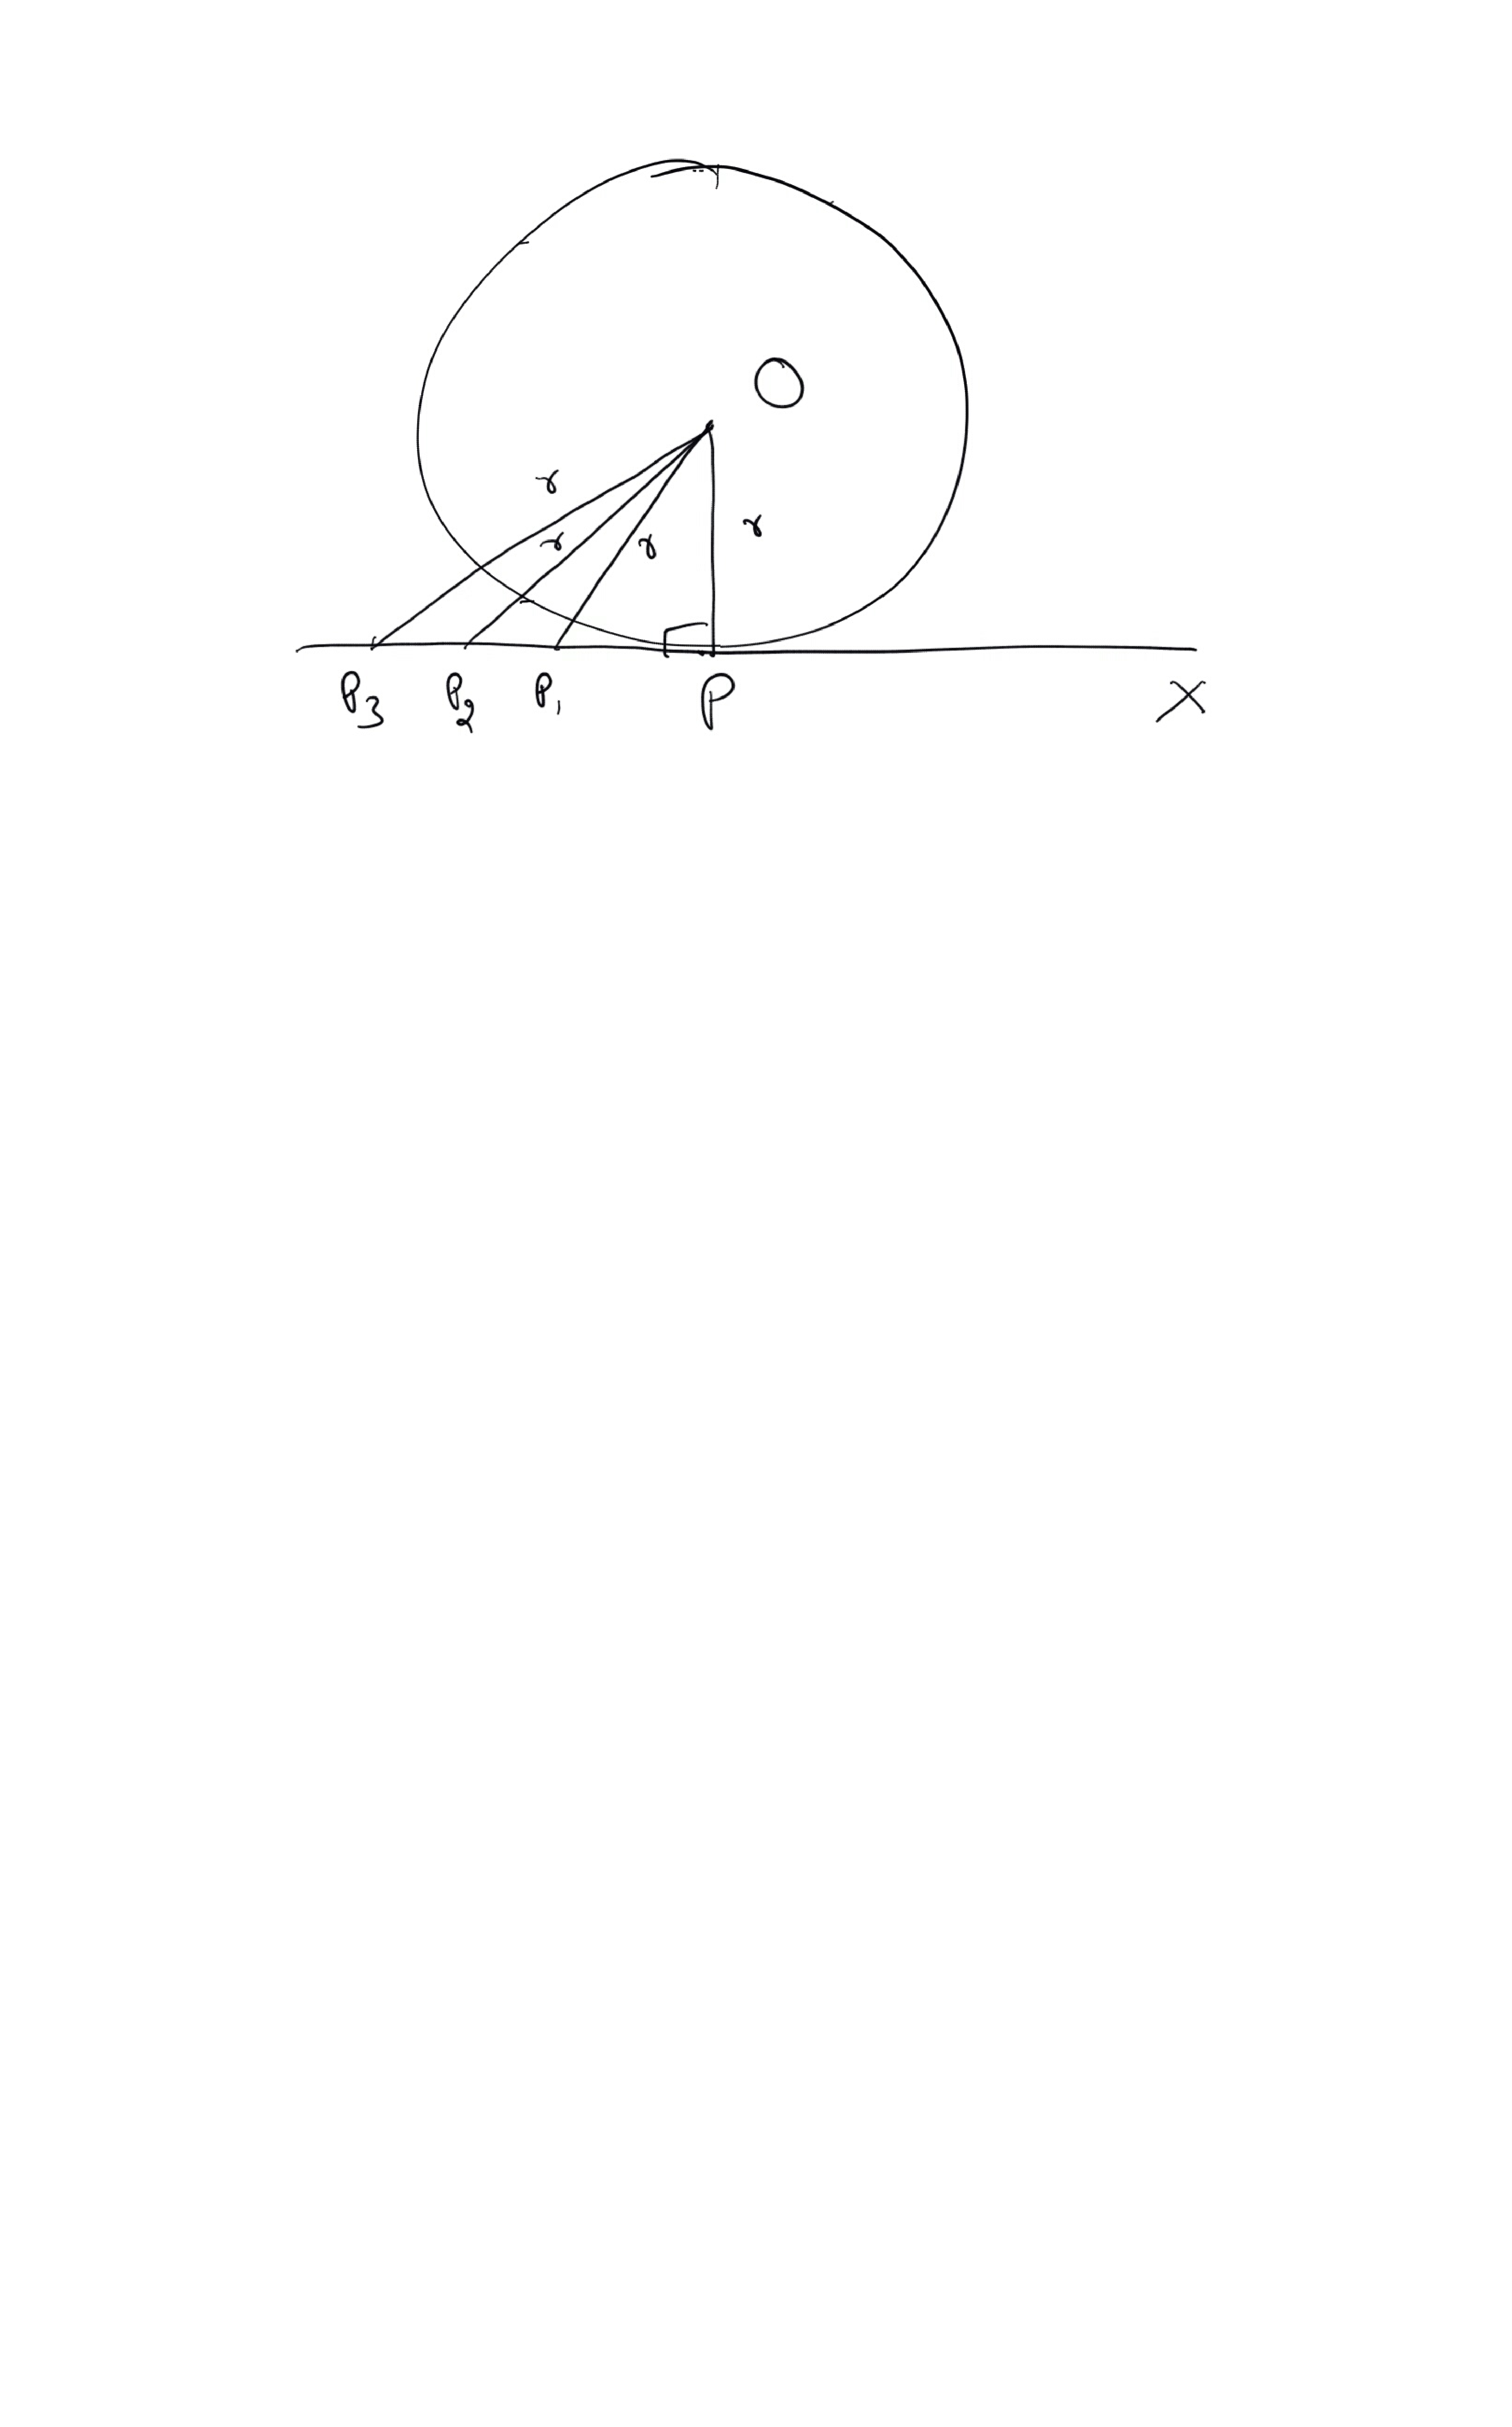
\includegraphics[width=\columnwidth]{./figs/ch4_tangent_def}
		\vspace*{-10cm}
	\end{center}
	\caption{Tangent to a Circle.}
	\label{ch4_tangent_def}	
\end{figure}
%
\begin{figure}[!h]
	\begin{center}
		
		
\includegraphics[width=\columnwidth]{./figs/ch4_short_dist}
		\vspace*{-10cm}
	\end{center}
	\caption{Shortest distance from $O$ to line $PX$}
	\label{ch4_short_dist}	
\end{figure}

%
\begin{equation}
\begin{split}
OP_1^2 &= OP^2 + PP_1^2 \\
\Rightarrow OP_1 > OP
\end{split}
\end{equation}
%
Thus, $OP$ is the shortest distance between $O$ and line $PX$.
%
\begin{problem}
Show that $\angle OPX = 90 ^{\degree}$
\end{problem}
\proof In Fig. \ref{ch4_tangent_def}, we can see that $OP$ is is the radius of the circle and the length of all line segments from $O$ to the line $PX > r$.  Using the result of the previous 
problem, it is obvious that $OP \perp PX$. 
%
	%
\begin{problem}
In Fig. \ref{ch4_tangent_prod} show that 
%
\begin{equation}
\angle PCA = \angle PBC
\end{equation}
%
$O$ is the centre of the circle and $PC$ is the tangent.
\end{problem}
	\begin{figure}[!h]
		\begin{center}
			
			
\includegraphics[width=\columnwidth]{./figs/ch4_tangent_prod}
			\vspace*{-10cm}
		\end{center}
		\caption{$PA.PB = PC^2$.}
		\label{ch4_tangent_prod}	
	\end{figure}
	%

%
\proof For convenience, greek letters are used for representing certain angles. Since $\Delta OAC$ is isosceles,
%
\begin{align}
2 \alpha + 2 \brak{\beta - \phi} &= 180^{\degree} \\
\Rightarrow  \alpha +  \brak{\beta - \phi} &= 90^{\degree} \\
\Rightarrow  \alpha +  \beta  &= 90^{\degree} + \phi
\end{align}
%
Since $theta$ is an exterior angle for the $\Delta ABC
$,
%
\begin{equation}
\theta = \alpha + \beta
\end{equation}
%
From both the above equations
%
\begin{equation}
\theta = 90^{\degree} + \phi
\end{equation}
%
Since PC is the tangent, 
%
\begin{equation}
\angle PCB = 90^{\degree} + \phi = \theta
\end{equation}
%
Considering the sum of angles in $\Delta PAC$ $\Delta PBC$,
%
\begin{align}
\angle P + \theta + \angle PCA &= 180^{\degree} \\
\angle P + \theta + \alpha &= 180^{\degree}
\end{align}
Hence,
%
\begin{equation}
\angle PCA = \alpha
\end{equation}
%
\begin{problem}
	In Fig. \ref{ch4_tangent_prod}, show that the triangles $PAC$ and $PBC$ are similar.
\end{problem}
\proof From the previous problem, it is obvious that corresponding angles of both triangles are equal.  Hence they are similar.
%
\begin{problem}
	Show that $PA.PB = PC^2$
\end{problem}
\proof Since $\Delta PAC \sim \Delta PBC$, their sides are in the same ratio.  Hence,
%
\begin{align}
\frac{PA}{PC} &= \frac{PC}{PB} \\
\Rightarrow PA.PB &=PC^2
\end{align}
%
%
\begin{problem}
	In Fig. \ref{ch4_chord_tangent_prod}, show that\begin{equation}
	PA.PB = PC.PD
	\end{equation}
\end{problem}
%
\begin{figure}[!h]
	\begin{center}
		
		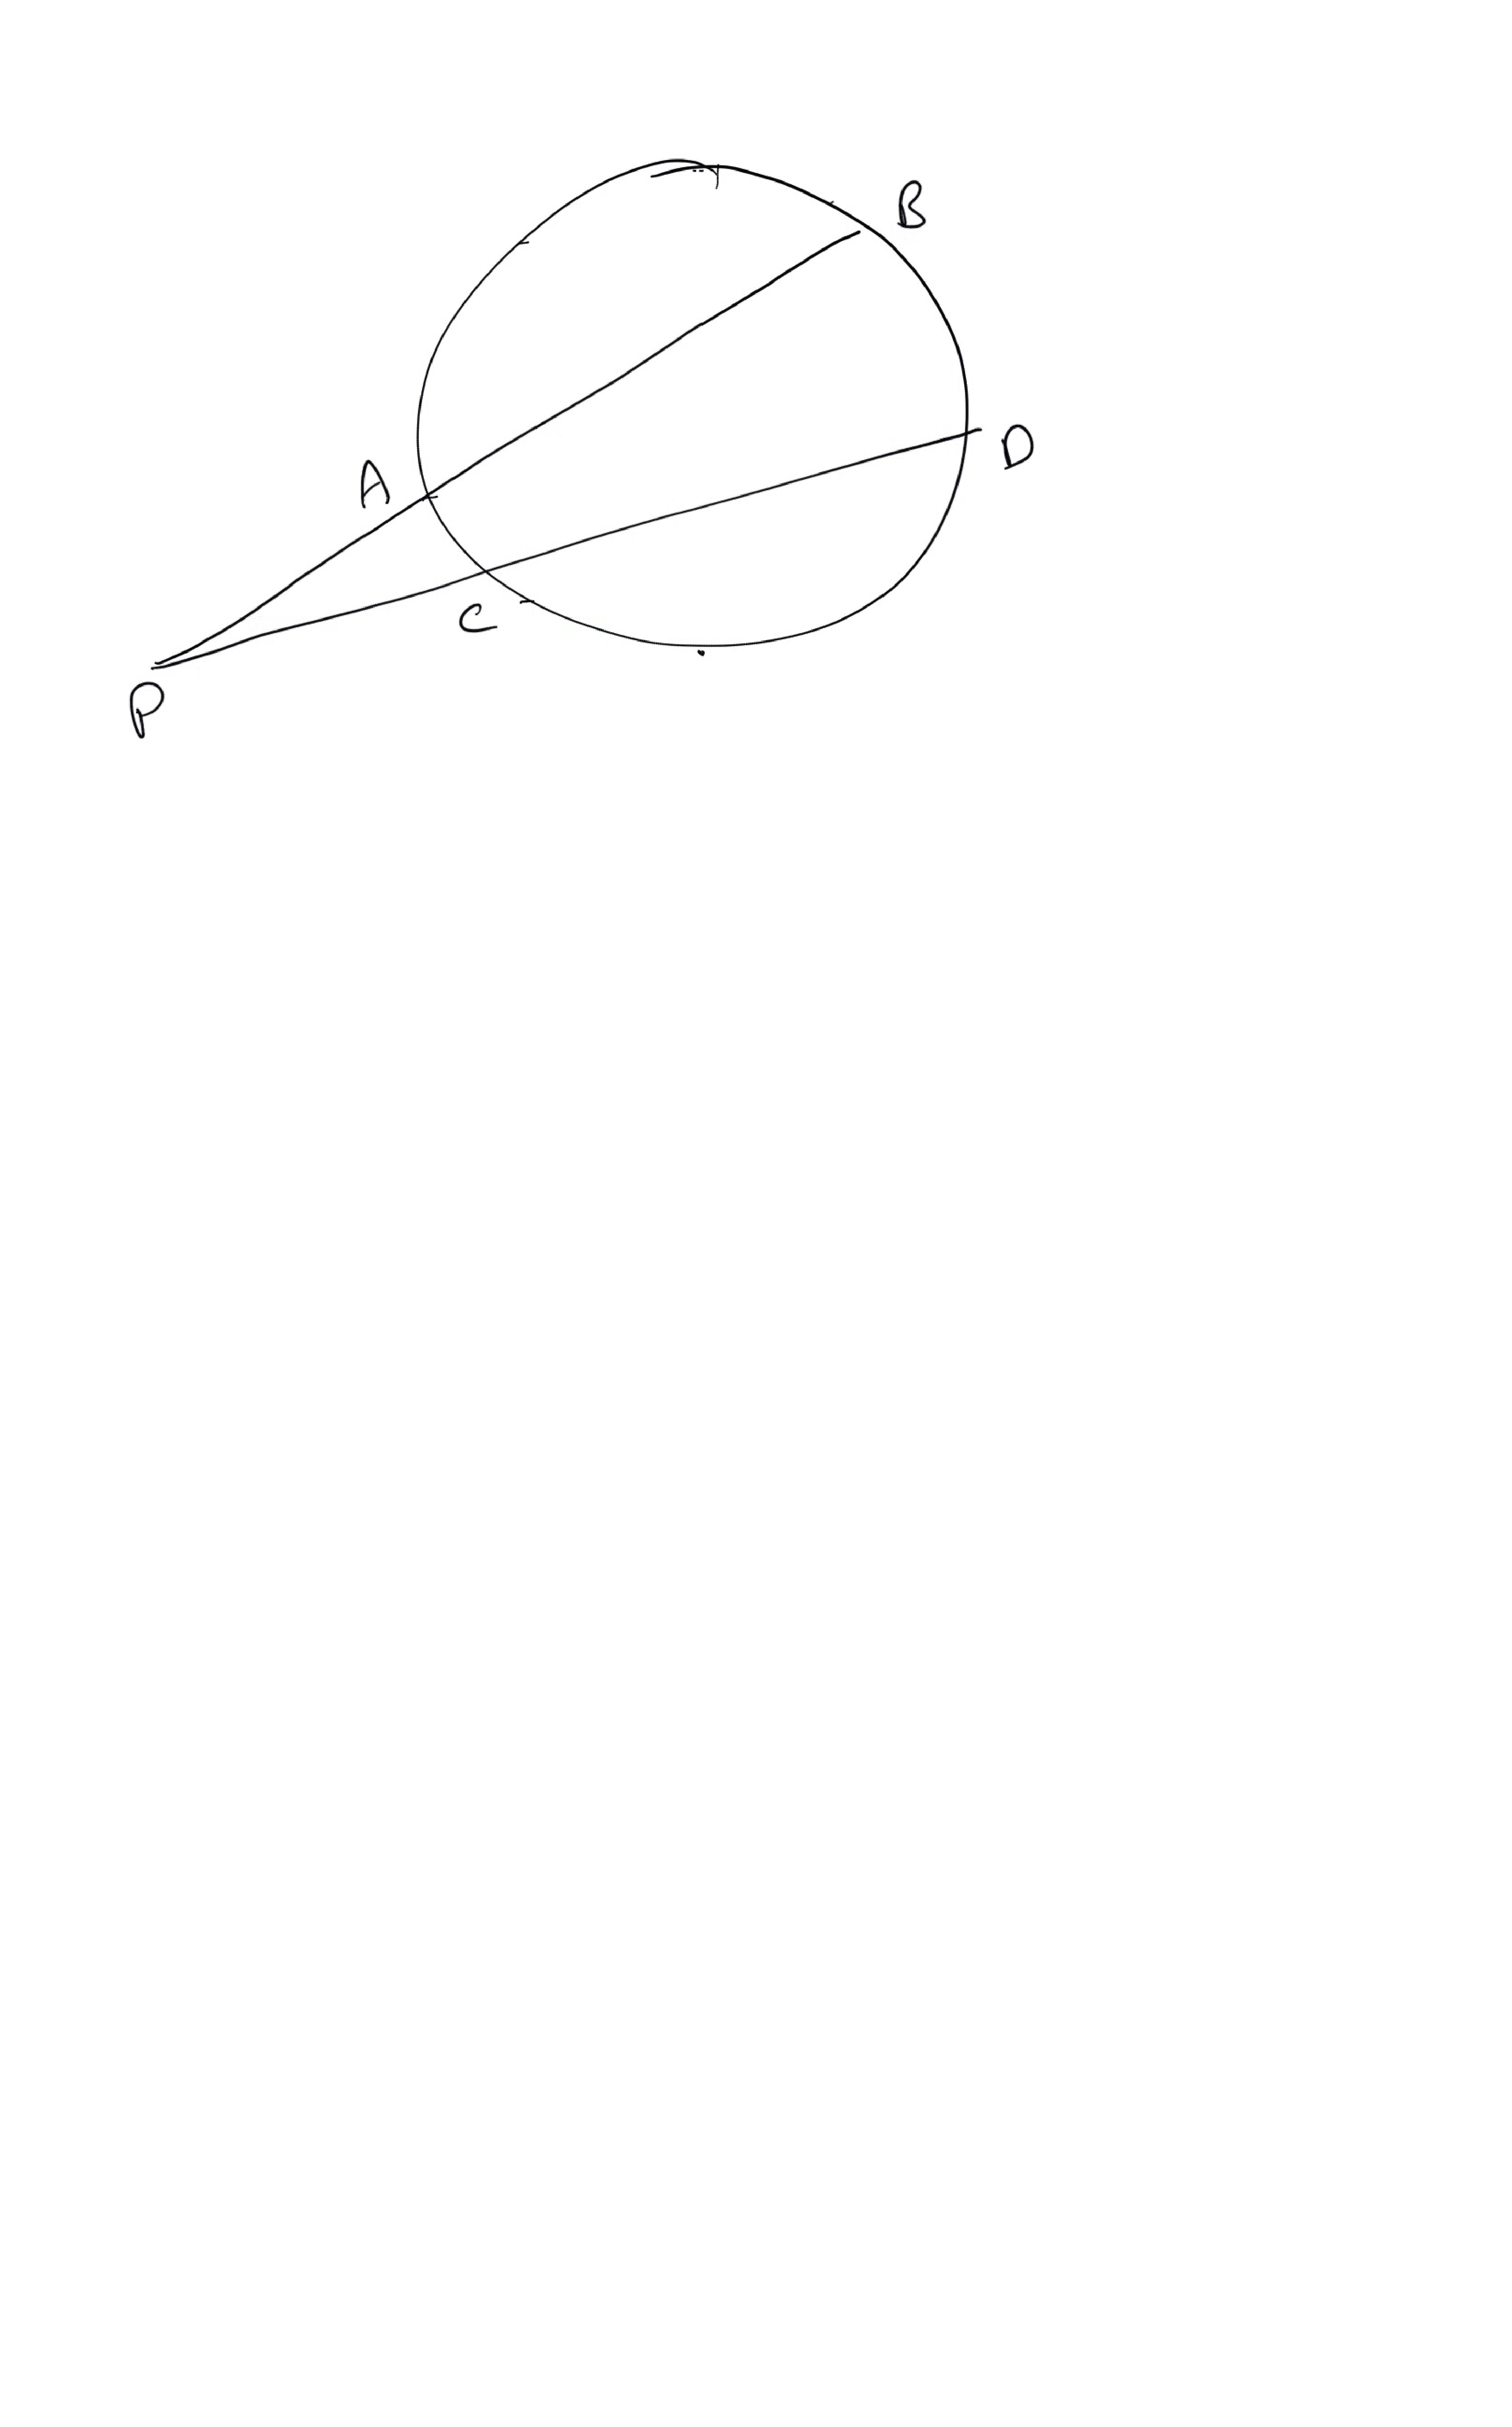
\includegraphics[width=\columnwidth]{./figs/ch4_chord_tangent_prod}
		\vspace*{-10cm}
	\end{center}
	\caption{$PA.PB = PC^2$.}
	\label{ch4_chord_tangent_prod}	
\end{figure}

\proof Draw a tangent and use the previous problem.

%
%\section{Area of a Circle}
%\subsection{The Regular Polygon}
%

\begin{definition}
	In Fig. \ref{ch5_polygon_def}, 6 congruent triangles are arranged in a circular fashion.  Such a figure is known as a regular hexagon.  In general, $n$ number of traingles can be arranged to form a regular polygon.
\end{definition}
\begin{figure}[!h]
	\begin{center}
		
		
\includegraphics[width=\columnwidth]{./figs/ch5_polygon_def}
		\vspace*{-10cm}
	\end{center}
	\caption{Polygon Definition}
	\label{ch5_polygon_def}	
\end{figure}
%
\begin{definition}
The angle formed by each of the congruent triangles at the centre of a regular polygon of $n$ sides is $\frac{360^{\degree}}{n}$.
\end{definition}
%
\begin{problem}
Show that the area of a regular polygon is given by 
%
\begin{equation}
\frac{n}{2}r^{2}\sin\frac{360^{\degree}}{n}
\end{equation}
%
\end{problem}
\begin{figure}[!h]
	\begin{center}
		
		
\includegraphics[width=\columnwidth]{./figs/ch5_polygon_area}
		\vspace*{-10cm}
	\end{center}
	\caption{Polygon Area}
	\label{ch5_polygon_area}	
\end{figure}
%

\proof The triangle that forms the polygon of $n$ sides is given in Fig. \ref{ch5_polygon_area}.  Thus,
%
\begin{equation}
\begin{split}
ar\brak{polygon} &= n ar\brak{\Delta ABC} \\
&= \frac{n}{2}r^{2}\sin\frac{360^{\degree}}{n}
\end{split}
\end{equation}
%
\begin{problem}
	Using Fig. \ref{ch5_circle_squeeze}, show that
%
\begin{equation}
\label{ch5_circle_squeeze_eq}
\frac{n}{2}r^{2}\sin\frac{360^{\degree}}{n} < \text{ area of circle } < nr^{2}\tan\frac{180^{\degree}}{n}
\end{equation}
%
The portion of the circle visible in Fig. \ref{ch5_circle_squeeze} is defined to be a sector of the circle.
\end{problem}
\begin{figure}[!h]
	\begin{center}
		
		
\includegraphics[width=\columnwidth]{./figs/ch5_circle_squeeze}
		\vspace*{-10cm}
	\end{center}
	\caption{Circle Area in between Area of Two Polygons}
	\label{ch5_circle_squeeze}	
\end{figure}
%

\proof Note that the circle is squeezed between the inner and outer regular polygons.  As we can see from Fig. \ref{ch5_circle_squeeze}, the area of the circle should be in between the areas of the inner and outer polygons.  Since
%
\begin{align}
ar \brak{\Delta OAB} &= \frac{1}{2}r^{2}\sin\frac{360^{\degree}}{n} \\
ar \brak{\Delta OPQ} &= 2 \times \frac{1}{2} \times r \tan\frac{360/n}{2} \times r \\
&= r^{2}\tan\frac{180^{\degree}}{n},
\end{align}
%
we obtain \eqref{ch5_circle_squeeze_eq}.
%
%
\begin{problem}
	Using Fig. \ref{ch5_sin_theta}, show that 
	%
\begin{equation}
\label{ch5_sin_theta_eq}
\sin  \theta_1 = \sin \brak{\theta_1 + \theta_2}\cos \theta_2 - \cos\brak{\theta_1+\theta_2}\sin\theta_2
\end{equation}	
	%
\end{problem}
\begin{figure}[!h]
	\begin{center}
		
		
\includegraphics[width=\columnwidth]{./figs/ch5_sin_theta}
		\vspace*{-10cm}
	\end{center}
	\caption{$\sin2\theta = 2\sin\theta\cos\theta$}
	\label{ch5_sin_theta}	
\end{figure}
%

\proof The following equations can be obtained from the figure using the forumula for the area of a triangle
%
\begin{align}
ar \brak{\Delta ABC} &= \frac{1}{2}ac \sin\brak{\theta_1 + \theta_2} \\
&= ar \brak{\Delta BDC} + ar \brak{\Delta ADB} \\
&= \frac{1}{2}cl \sin{\theta_1} + \frac{1}{2}al \sin{\theta_2} \\ 
&= \frac{1}{2}ac \sin{\theta_1} \sec \theta_2 + \frac{1}{2}a^2 \tan{\theta_2} 
\end{align}
$\brak{\because
	l = a \sec \theta_2}$.  From the above,
\begin{align}
\Rightarrow \sin\brak{\theta_1 + \theta_2} &=  \sin{\theta_1} \sec \theta_2 + \frac{a}{c} \tan{\theta_2} \\
\Rightarrow \sin\brak{\theta_1 + \theta_2} &=  \sin{\theta_1} \sec \theta_2 + \cos\brak{\theta_1 + \theta_2} \tan{\theta_2} 
\end{align}
Multiplying both sides by $\cos \theta_2$,
\begin{align}
\Rightarrow \sin\brak{\theta_1 + \theta_2}\cos{\theta_2} &=  \sin{\theta_1}  + \cos\brak{\theta_1 + \theta_2} \sin\theta_2  
\end{align}
%
resulting in
\begin{equation}
\Rightarrow \sin \theta_1 = \sin\brak{\theta_1 + \theta_2}\cos{\theta_2} - \cos\brak{\theta_1 + \theta_2} \sin\theta_2 
\end{equation}
\begin{problem}
	Prove the following identities 
	%
	\begin{enumerate}
\item 
\begin{equation}
		\label{ch5_sin_diff}
\sin\brak{\alpha - \beta} = \sin \alpha \cos \beta - \cos \alpha \sin \beta.
\end{equation}
\item 
\begin{equation}
\cos\brak{\alpha + \beta} = \cos \alpha \cos \beta - \sin \alpha \sin \beta.
		\label{ch5_cos_diff}
\end{equation}

	\end{enumerate}
	%
\end{problem}
\proof In \eqref{ch5_sin_theta_eq}, let
%
\begin{equation}
\begin{split}
\theta_1 + \theta_2 &= \alpha \\
\theta_2 &=  \beta
\end{split}
\end{equation}
%
This gives \eqref{ch5_sin_diff}.  In \eqref{ch5_sin_diff}, replace $\alpha$ by 
%
$90^{\degree} - \alpha$.  This results in
%
\begin{multline}
\sin\brak{90^{\degree} - \alpha - \beta}
\\
=
\sin \brak{90^{\degree} -\alpha} \cos \beta - \cos \brak{90^{\degree} -\alpha} \sin \beta \\
\Rightarrow \cos\brak{\alpha + \beta} = \cos \alpha \cos \beta - \sin \alpha \sin \beta
\end{multline}
% 
\begin{problem}
	Using \eqref{ch5_sin_theta_eq} and \eqref{ch5_cos_diff}, show that
\begin{align}
\label{ch5_sin_sum}
\sin\brak{\theta_1 + \theta_2} &= \sin\theta_1  \cos\theta_2 + \cos\theta_1\sin\theta_2
\\
\cos\brak{\theta_1 - \theta_2} &= \cos\theta_1  \cos\theta_2  \sin\theta_1\sin\theta_2
\label{ch5_cos_sum}
\end{align}
\end{problem}
%
\proof From \eqref{ch5_sin_theta_eq},
%
\begin{align}
 \sin \brak{\theta_1 + \theta_2}\cos \theta_2 =\sin  \theta_1 +\cos\brak{\theta_1+\theta_2}\sin\theta_2 
\end{align}
%
Using \eqref{ch5_cos_diff} in the above,
%
\begin{multline}
\sin \brak{\theta_1 + \theta_2}\cos \theta_2 
=\sin  \theta_1 +\lbrak{\cos \theta_1\cos\theta_2 }
\\	
\rbrak{	- \sin \theta_1\sin\theta_2}\sin\theta_2 
\end{multline}
%
which can be expressed as
%
\begin{multline}
\sin \brak{\theta_1 + \theta_2}\cos \theta_2 
=\sin  \theta_1 +\cos \theta_1\cos\theta_2 \sin\theta_2 
\\	
	- \sin \theta_1\sin^2\theta_2
\end{multline}
%
Since
%
\begin{equation}
\sin^2\theta_2 = 1- \cos^2\theta_2, 
\end{equation}
%
we obtain
%
\begin{multline}
\sin \brak{\theta_1 + \theta_2}\cos \theta_2 
=\cos \theta_1\cos\theta_2 \sin\theta_2 
\\	
+ \sin \theta_1\cos^2\theta_2
\end{multline}
%
resulting in
%
\begin{equation}
\sin \brak{\theta_1 + \theta_2}
=\cos \theta_1 \sin\theta_2 
+ \sin \theta_1\cos\theta_2
\end{equation}
%
after factoring out $\cos \theta_2$.  Using a similar approach, \eqref{ch5_cos_sum} can also be proved.
%
\begin{problem}
	Show that
	%
	\begin{equation}
	\label{eq:sin2theta}
	\sin 2\theta = 2 \sin\theta \cos\theta
	\end{equation}
	%
\end{problem}
\begin{problem}
Show that
	%
	\begin{equation}
	\label{ch5_circle_squeeze_simple}
\cos^2\frac{180^{\degree}}{n} < \frac{\text{ area of circle }}{nr^{2}\tan\frac{180^{\degree}}{n}} < 1	\end{equation}
	%
\end{problem}
\proof From \eqref{ch5_circle_squeeze_eq} and \eqref{eq:sin2theta},
	%
	\begin{multline}
	\frac{n}{2}r^{2}\sin\frac{360^{\degree}}{n} < \text{ area of circle } 
	\\
	< nr^{2}\tan\frac{180^{\degree}}{n} 
	\\
\Rightarrow 	
	{n}r^{2}\sin\frac{180^{\degree}}{n}\cos\frac{180^{\degree}}{n} < \text{ area of circle } 
	\\
	< nr^{2}\tan\frac{180^{\degree}}{n} 
	\end{multline}
	%
\begin{problem}
	Show that if
\begin{equation}
\label{ch5_sin_increasing}
\theta_1 < \theta_2, \sin \theta_1 < \sin \theta_2.
\end{equation}	
\end{problem}
\proof Trivial using the definition and choosing angles $\theta_1$ and $\theta_2$ appropriately in a right angled triangle.
%
	%
	\begin{problem}
		Show that if
		\begin{equation}
		\label{ch5_sin_increasing}
		\theta_1 < \theta_2, \cos \theta_1 > \cos \theta_2.
		\end{equation}	
	\end{problem}
	%
\begin{problem}
	Show that 
	\begin{equation}
	\label{ch5_sin_zero}
	\sin 0^{\degree} = 0
	\end{equation}
\end{problem}
\proof Follows from \eqref{ch5_sin_increasing}.
%
\begin{problem}
	Show that 
	\begin{equation}
	\label{ch5_sin_zero}
	\cos 0^{\degree} = 1
	\end{equation}
	\end{problem}
%
%
\begin{problem}
	Show that for large values of $n$
	%
	\begin{equation}
	%
\cos^2\frac{180^{\degree}}{n} = 1
%
	\end{equation}	
	% 
\end{problem}
%
\proof  Follows from previous problem.
%
\begin{definition}
	The previous result can be expressed as
%
\begin{equation}
\lim_{n \rightarrow \infty}\cos^2\frac{180^{\degree}}{n} = 1
\end{equation}
%	
\end{definition}
\begin{problem}
	Show that 
	%
\begin{equation}
\text{ area of circle } = r^2\lim_{n \rightarrow \infty}
{n\tan\frac{180^{\degree}}{n}} 
	%
\end{equation}	
	% 
\end{problem}
%
\begin{definition}
	\begin{equation}
	\pi = \lim_{n \rightarrow \infty}
	{n\tan\frac{180^{\degree}}{n}}
	\end{equation}
\end{definition}
Thus, the area of a circle is $\pi r^2$.
\begin{definition}
	The radian is a unit of angle defined by
\begin{equation}
	1 \text{ radian} = \frac{360^{\degree}}{2\pi}
\end{equation}
\end{definition}
%
\begin{problem}
	Show that the circumference of a circle is $2 \pi r$.
\end{problem}
\begin{problem}
	Show that the area of a sector with angle $\theta$ in radians is $\frac{1}{2}r^2\theta$.
\end{problem}
\begin{problem}
	Show that
	\begin{equation}
	\lim_{\theta \rightarrow 0} \frac{\sin\theta}{\theta} = 1
	\end{equation}
\end{problem}



%\newpage
%\section{Linear Programming}
%\subsection{Chord of a Circle}

\begin{figure}[!h]
	\begin{center}
		
		
\includegraphics[width=\columnwidth]{./figs/ch4_circle_def}
		\vspace*{-10cm}
	\end{center}
	\caption{Circle Definitions}
	\label{ch4_circle_def}	
\end{figure}
\begin{definition}
	Fig. \ref{ch4_circle_def} represents a circle.  The points in the circle are at a distance $r$ from the centre $O$.  $r$ is known as the radius.
\end{definition}

\subsection{Chords of a circle}
\begin{definition}
	In Fig. \ref{ch4_circle_def}, $A$ and $B$ are points on the circle.  The line $AB$ is known as a chord of the circle.
\end{definition}
%
%
\begin{problem}
	\label{ch4_prob_circle_subtend}
	In Fig. \ref{ch4_circle_subtend}  Show that $\angle OAB = 2\angle APB $.
\end{problem}
\begin{figure}[!h]
	\begin{center}
		
		
\includegraphics[width=\columnwidth]{./figs/ch4_circle_subtend}
		\vspace*{-10cm}
	\end{center}
	\caption{Angle subtended by chord $AB$ at the centre $O$ is twice the angle subtended at $P$. }
	\label{ch4_circle_subtend}	
\end{figure}

\proof In Fig. \ref{ch4_circle_subtend}, the triangeles $OPA$ and $OPB$ are isosceles. Hence,
%
\begin{align}
\angle OPB = \angle OBP &= \theta_1 \\
\angle OPA = \angle OAP &= \theta_2
\end{align}
%
Also, $\alpha$ and $\beta$ are exterior angles corresponding to the triangle $OPB$ and $OPA$ respectively. Hence
%
\begin{align}
\alpha &= 2\theta_1 \\
\beta &= 2\theta_2
\end{align}
%
Thus,
%
\begin{align}
\angle AOB &= \alpha + \beta \\
&= \theta_1 + \theta_2 \\
&= \angle APB
\end{align}
%
\begin{definition}
	The diameter of a circle is the chord that divides the circle into two equal parts. In Fig. \ref{ch4_circle_dia}, $AB$ is the diameter and passes through the centre $O$
\end{definition}
%
\begin{problem}
In Fig. \ref{ch4_circle_dia}, show that $\angle APB = 90^{\degree}$ .
\end{problem}
%
\begin{figure}[!h]
	\begin{center}
		
		
\includegraphics[width=\columnwidth]{./figs/ch4_circle_dia}
		\vspace*{-10cm}
	\end{center}
	\caption{Diameter of a circle.}
	\label{ch4_circle_dia}	
\end{figure}

\begin{problem}
	In Fig. \ref{ch4_chord_product}, show that 
	\begin{equation}
	\begin{split}
\angle ABD &= \angle ACD \\
\angle CAB &= \angle CDB	
	\end{split}
	\end{equation}
\end{problem}
\begin{figure}[!h]
	\begin{center}
		
		
\includegraphics[width=\columnwidth]{./figs/ch4_chord_product}
		\vspace*{-10cm}
	\end{center}
	\caption{$PA.PB = PC.PD$}
	\label{ch4_chord_product}	
\end{figure}
%
%
\proof Use Problem \ref{ch4_prob_circle_subtend}.
%
\begin{problem}
	In Fig. \ref{ch4_chord_product}, show that the triangles $PAB$ and $PBD$ are similar
\end{problem}
\proof Trivial using previous problem
\begin{problem}
	In Fig. \ref{ch4_chord_product}, show that 
	\begin{equation}
	PA.PB = PC.PD
	\end{equation}
\end{problem}
%
\proof Since triangles $PAC$ and $PBD$ are similar, 
%
\begin{align}
\frac{PA}{PD} &= \frac{PC}{PB} \\
\Rightarrow PA.PB &= PC.PD
\end{align}
%
%
\begin{definition}
	The line $PX$ in Fig. \ref{ch4_tangent_def} touches the circle at exactly one  point $P$. It is known as the tangent to the circle.
\end{definition}
%
%
\begin{problem}
	$OP$ is the perpendicular to the line $PX$ as shown in the Fig. \ref{ch4_short_dist}. Show that $OP$ is the shortest distance between the point $O$ and the line $PX$. 
\end{problem}
\proof Let $P_1$ be a point on the line $PX$. Then $OPP_1$ is a right angled triangle.  Using Budhayana's theorem,
%
\begin{figure}[!h]
	\begin{center}
		
		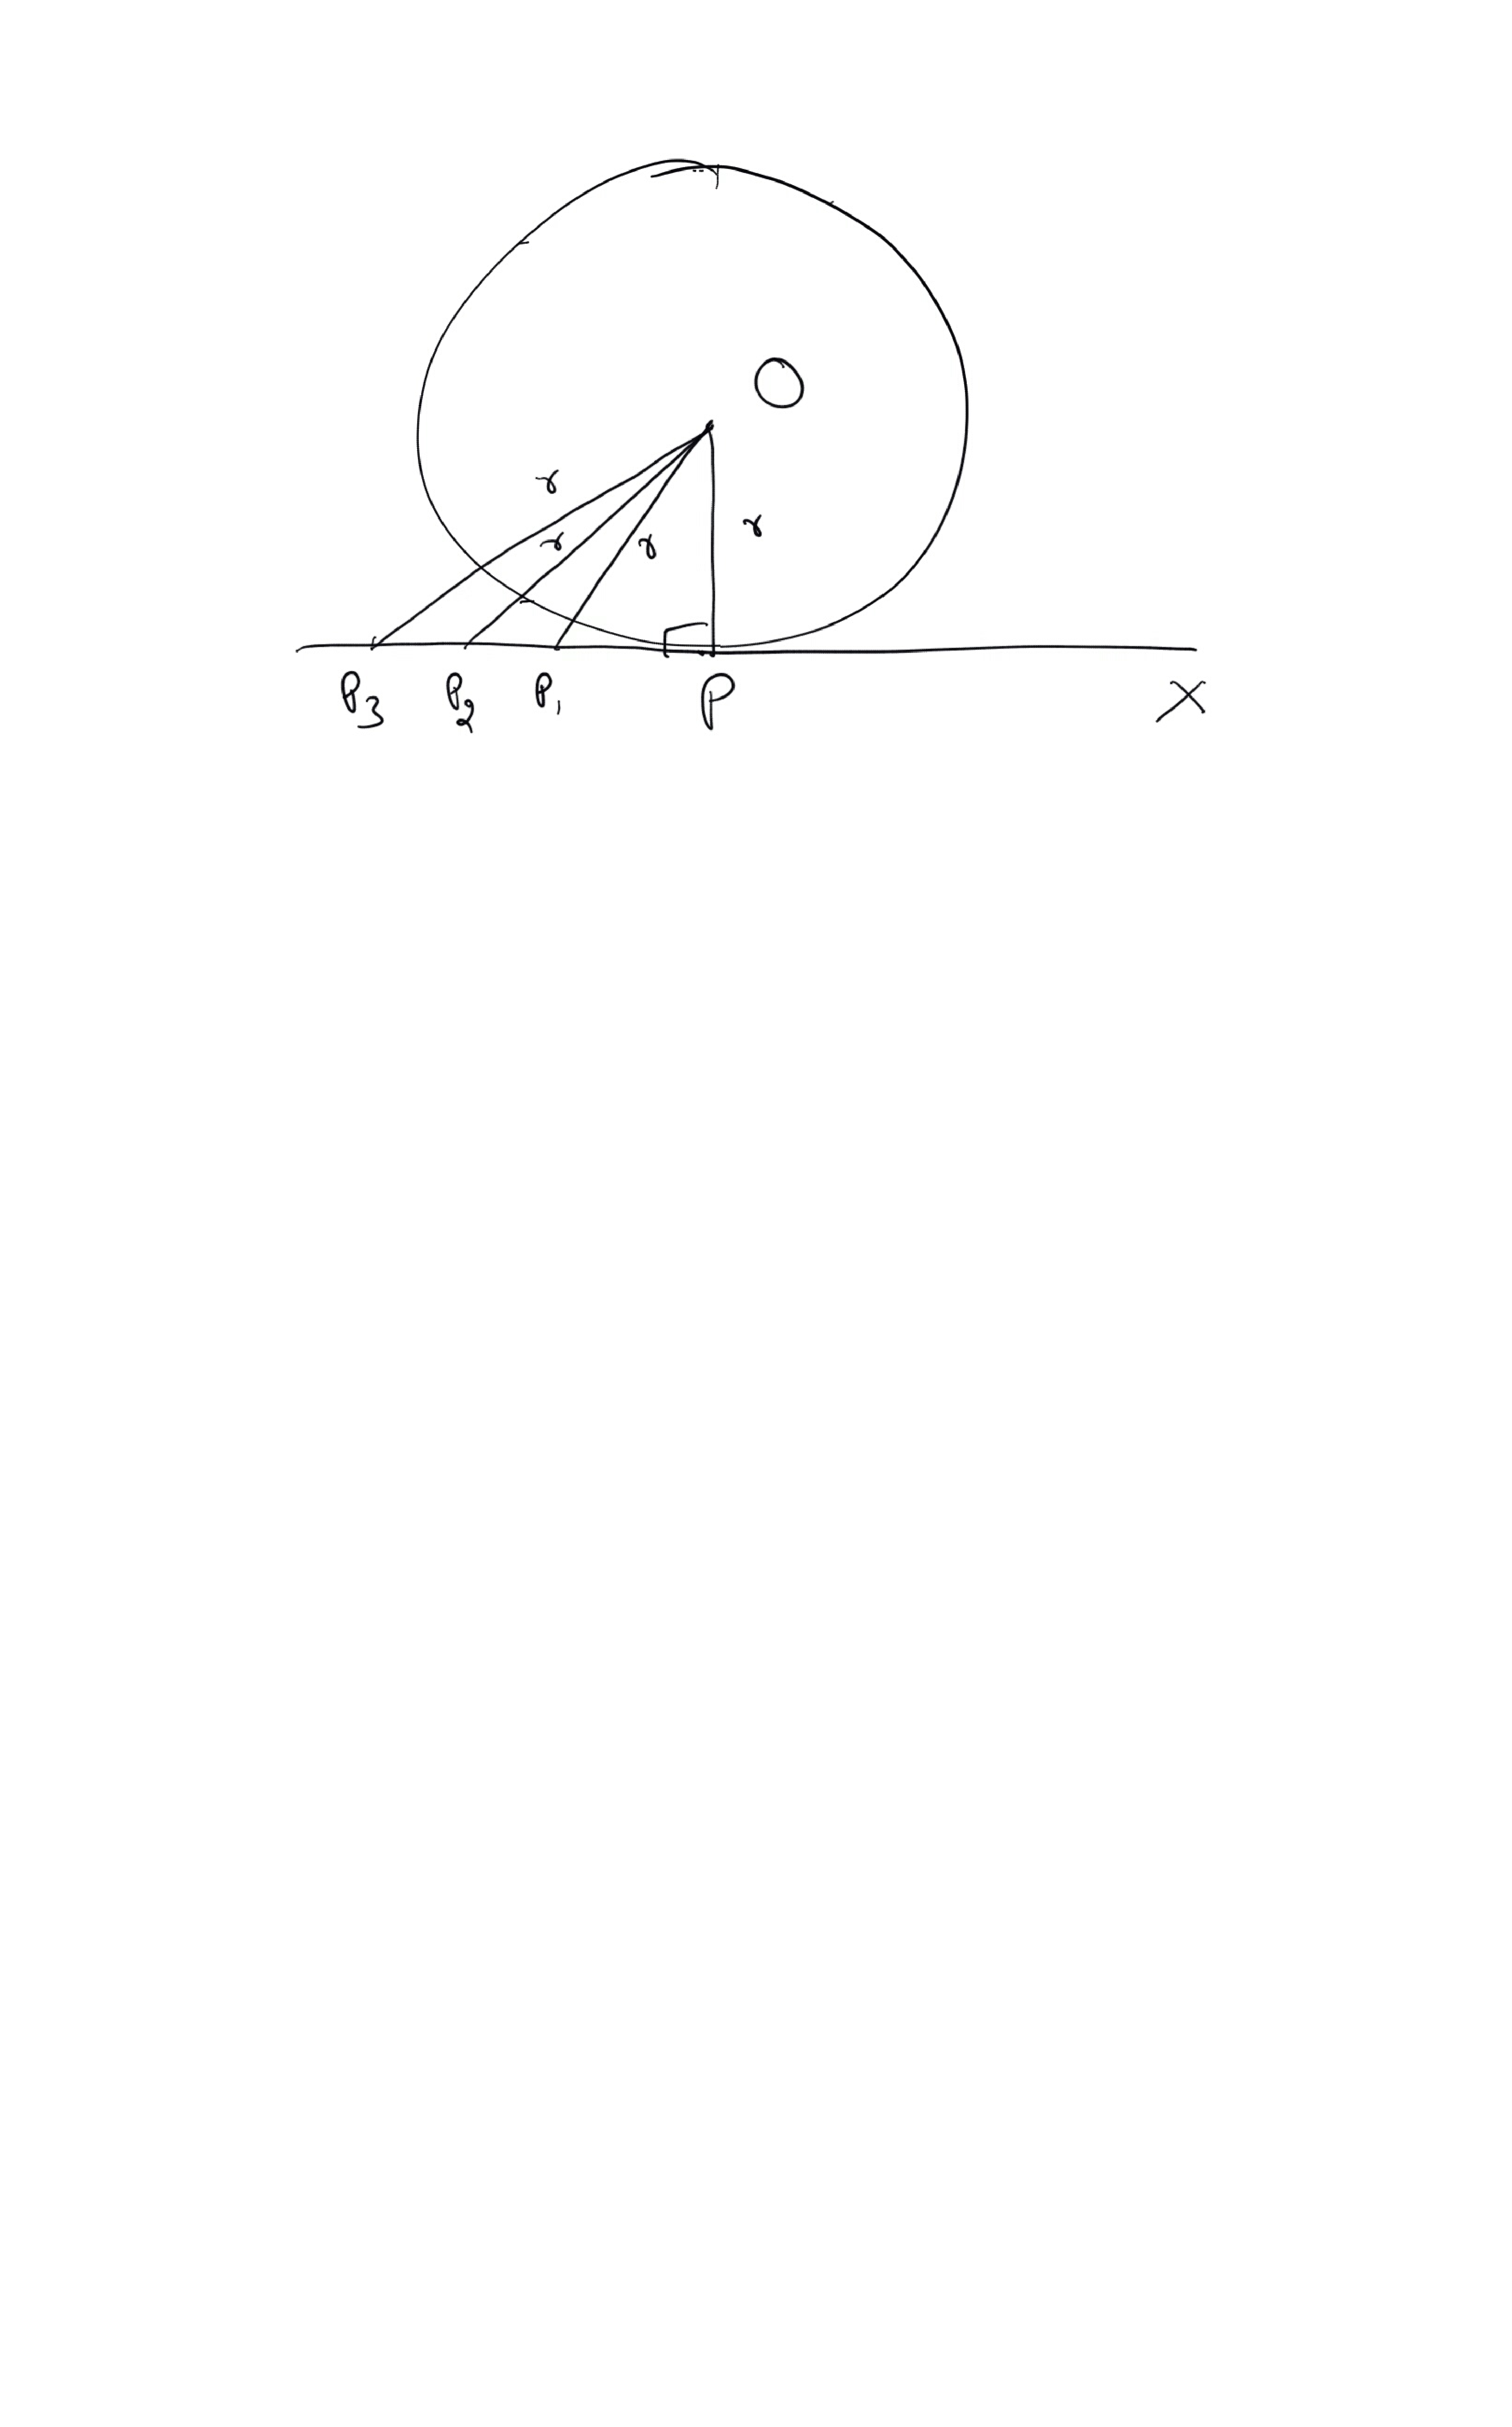
\includegraphics[width=\columnwidth]{./figs/ch4_tangent_def}
		\vspace*{-10cm}
	\end{center}
	\caption{Tangent to a Circle.}
	\label{ch4_tangent_def}	
\end{figure}
%
\begin{figure}[!h]
	\begin{center}
		
		
\includegraphics[width=\columnwidth]{./figs/ch4_short_dist}
		\vspace*{-10cm}
	\end{center}
	\caption{Shortest distance from $O$ to line $PX$}
	\label{ch4_short_dist}	
\end{figure}

%
\begin{equation}
\begin{split}
OP_1^2 &= OP^2 + PP_1^2 \\
\Rightarrow OP_1 > OP
\end{split}
\end{equation}
%
Thus, $OP$ is the shortest distance between $O$ and line $PX$.
%
\begin{problem}
Show that $\angle OPX = 90 ^{\degree}$
\end{problem}
\proof In Fig. \ref{ch4_tangent_def}, we can see that $OP$ is is the radius of the circle and the length of all line segments from $O$ to the line $PX > r$.  Using the result of the previous 
problem, it is obvious that $OP \perp PX$. 
%
	%
\begin{problem}
In Fig. \ref{ch4_tangent_prod} show that 
%
\begin{equation}
\angle PCA = \angle PBC
\end{equation}
%
$O$ is the centre of the circle and $PC$ is the tangent.
\end{problem}
	\begin{figure}[!h]
		\begin{center}
			
			
\includegraphics[width=\columnwidth]{./figs/ch4_tangent_prod}
			\vspace*{-10cm}
		\end{center}
		\caption{$PA.PB = PC^2$.}
		\label{ch4_tangent_prod}	
	\end{figure}
	%

%
\proof For convenience, greek letters are used for representing certain angles. Since $\Delta OAC$ is isosceles,
%
\begin{align}
2 \alpha + 2 \brak{\beta - \phi} &= 180^{\degree} \\
\Rightarrow  \alpha +  \brak{\beta - \phi} &= 90^{\degree} \\
\Rightarrow  \alpha +  \beta  &= 90^{\degree} + \phi
\end{align}
%
Since $theta$ is an exterior angle for the $\Delta ABC
$,
%
\begin{equation}
\theta = \alpha + \beta
\end{equation}
%
From both the above equations
%
\begin{equation}
\theta = 90^{\degree} + \phi
\end{equation}
%
Since PC is the tangent, 
%
\begin{equation}
\angle PCB = 90^{\degree} + \phi = \theta
\end{equation}
%
Considering the sum of angles in $\Delta PAC$ $\Delta PBC$,
%
\begin{align}
\angle P + \theta + \angle PCA &= 180^{\degree} \\
\angle P + \theta + \alpha &= 180^{\degree}
\end{align}
Hence,
%
\begin{equation}
\angle PCA = \alpha
\end{equation}
%
\begin{problem}
	In Fig. \ref{ch4_tangent_prod}, show that the triangles $PAC$ and $PBC$ are similar.
\end{problem}
\proof From the previous problem, it is obvious that corresponding angles of both triangles are equal.  Hence they are similar.
%
\begin{problem}
	Show that $PA.PB = PC^2$
\end{problem}
\proof Since $\Delta PAC \sim \Delta PBC$, their sides are in the same ratio.  Hence,
%
\begin{align}
\frac{PA}{PC} &= \frac{PC}{PB} \\
\Rightarrow PA.PB &=PC^2
\end{align}
%
%
\begin{problem}
	In Fig. \ref{ch4_chord_tangent_prod}, show that\begin{equation}
	PA.PB = PC.PD
	\end{equation}
\end{problem}
%
\begin{figure}[!h]
	\begin{center}
		
		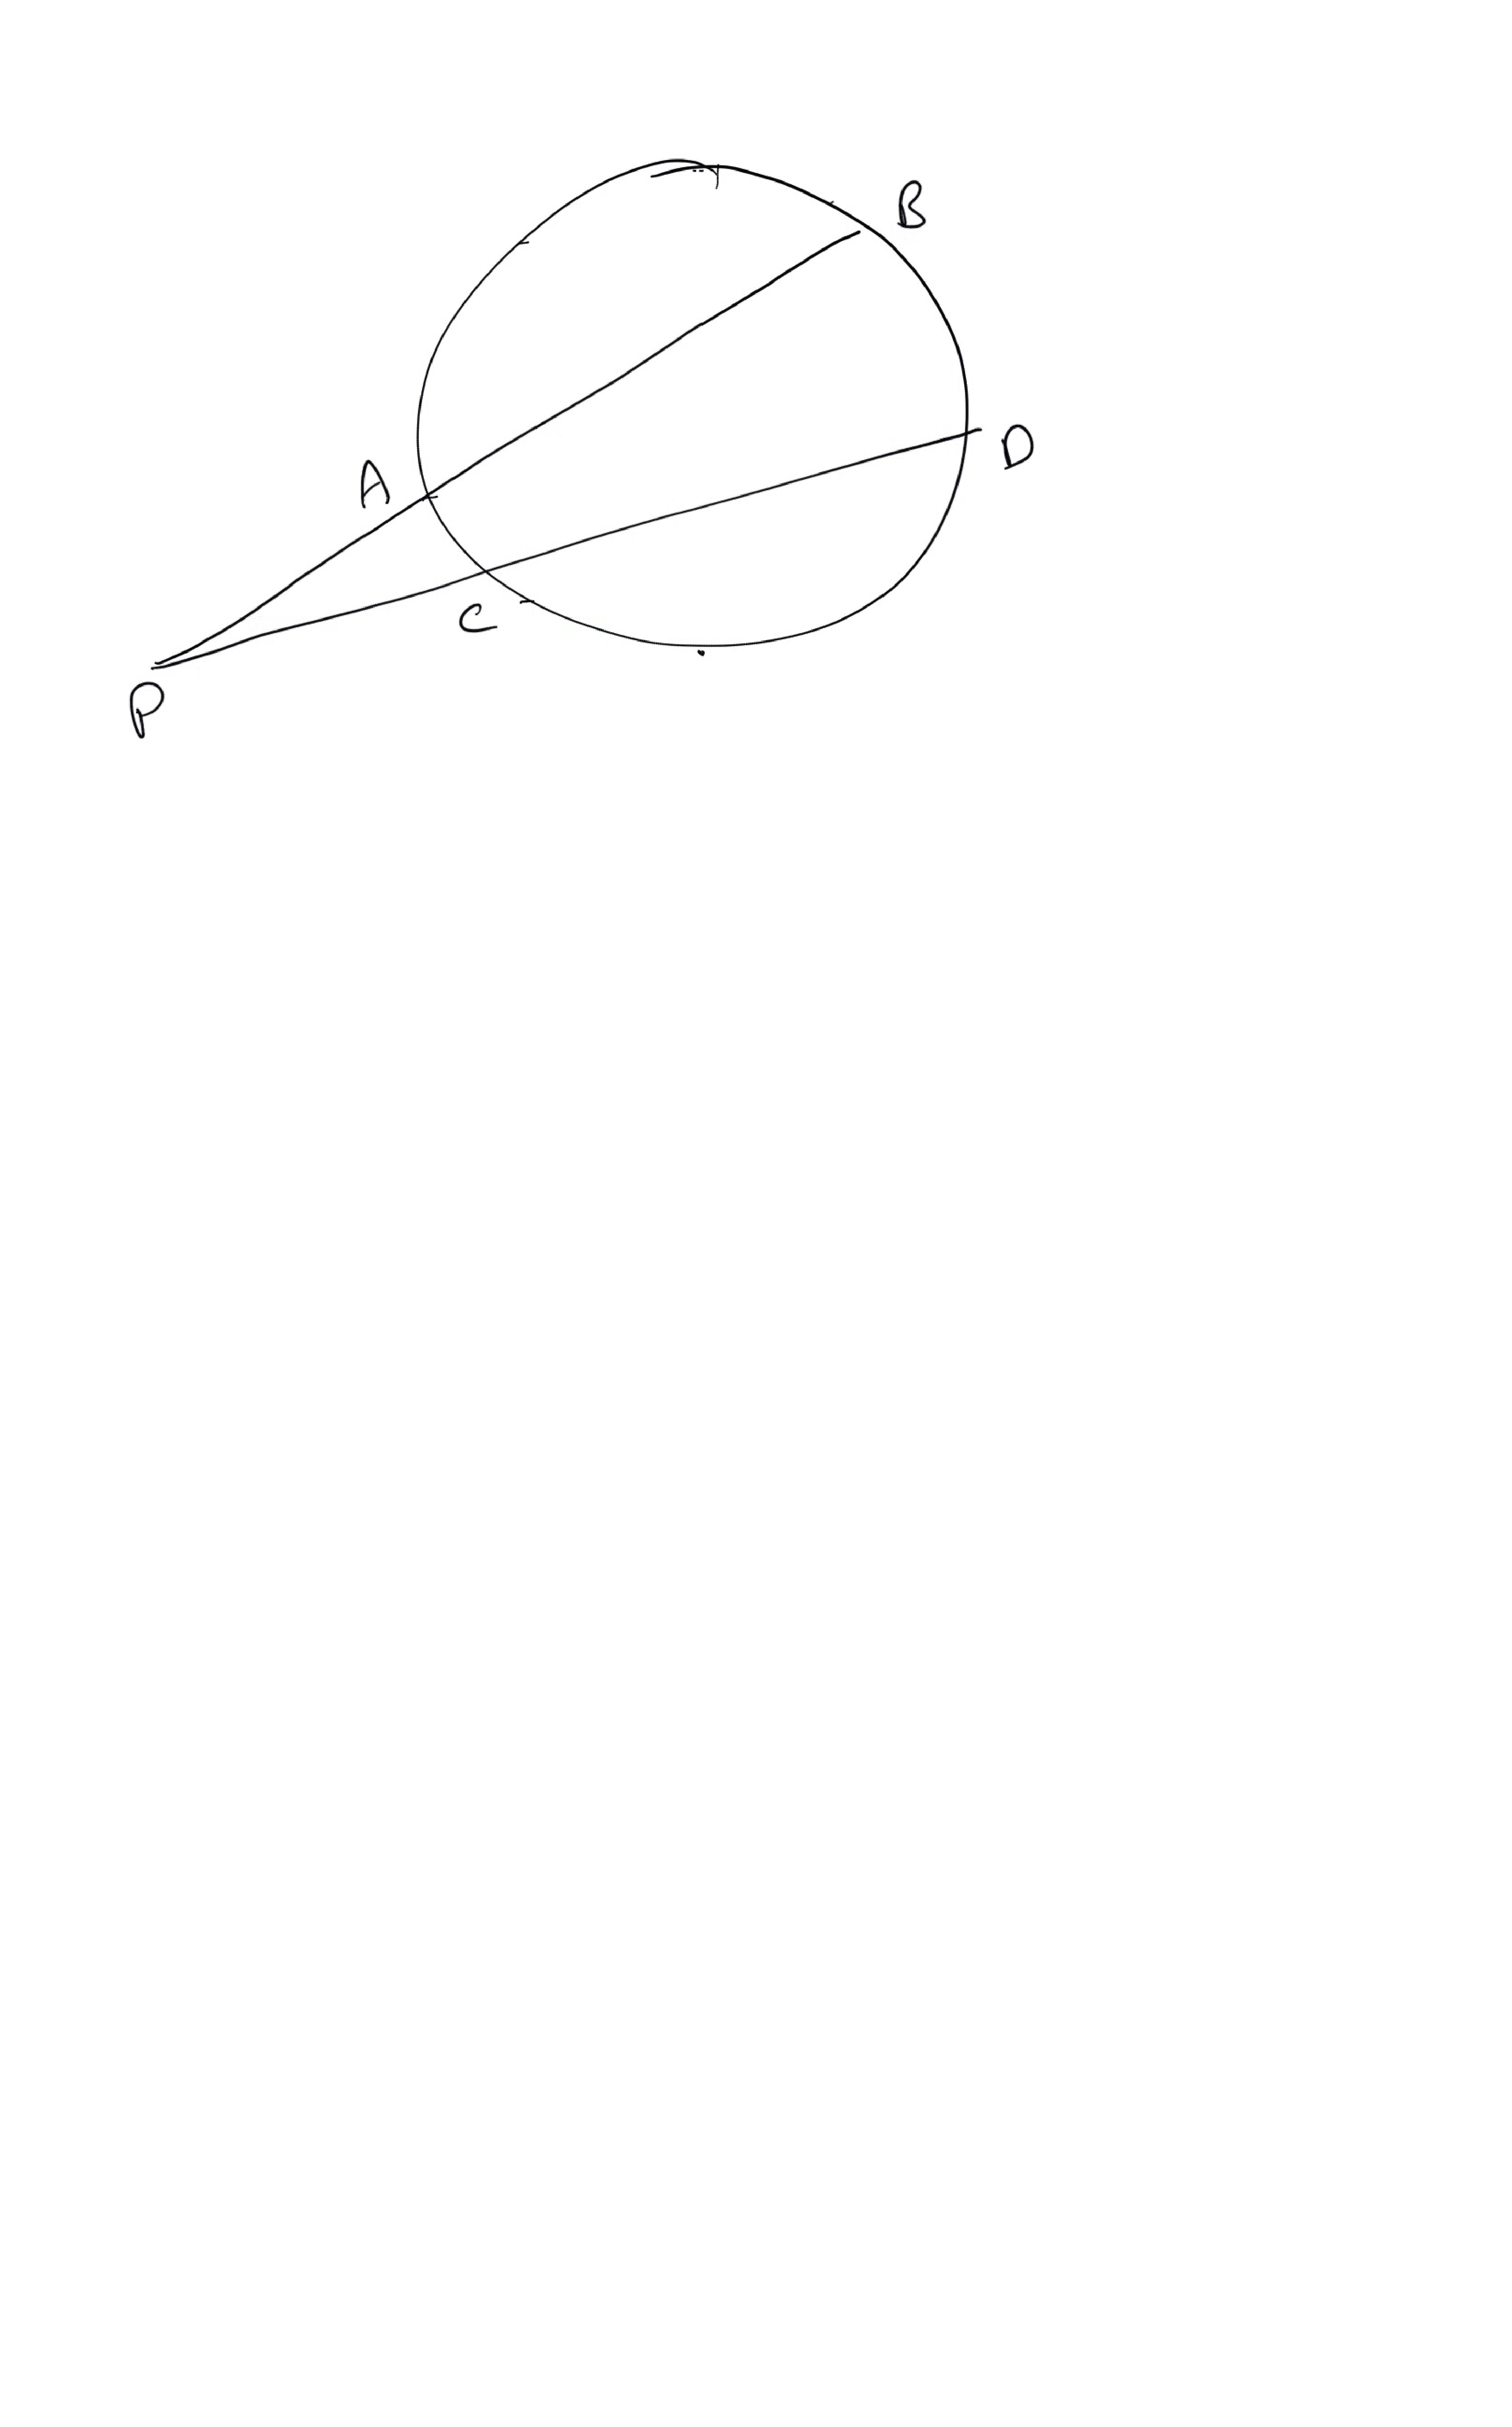
\includegraphics[width=\columnwidth]{./figs/ch4_chord_tangent_prod}
		\vspace*{-10cm}
	\end{center}
	\caption{$PA.PB = PC^2$.}
	\label{ch4_chord_tangent_prod}	
\end{figure}

\proof Draw a tangent and use the previous problem.


%\newpage
%\section{Application in Research}
%\input{revision}


%\bibliography{IEEEabrv,gvv_opt}

%\subsection{Driving the Segments}
%Open the arduino software.  Check if the ports show Arduino Uno and click the appropriate button.  
\begin{problem}
%Connect the A-D pins of the 7447 IC to the pins D2-D5 of the Arduino.
%Connect the A-D pins of the 7447 IC  in Fig. \ref{fig:7447} to the GPIO pins  0-3 of the Pi shown in Figs. \ref{fig_1_3a} and \ref{fig_1_3b}.
\end{problem}	
\renewcommand{\thefigure}{\theproblem.\arabic{figure}}
\begin{figure}[!ht]
\begin{center}
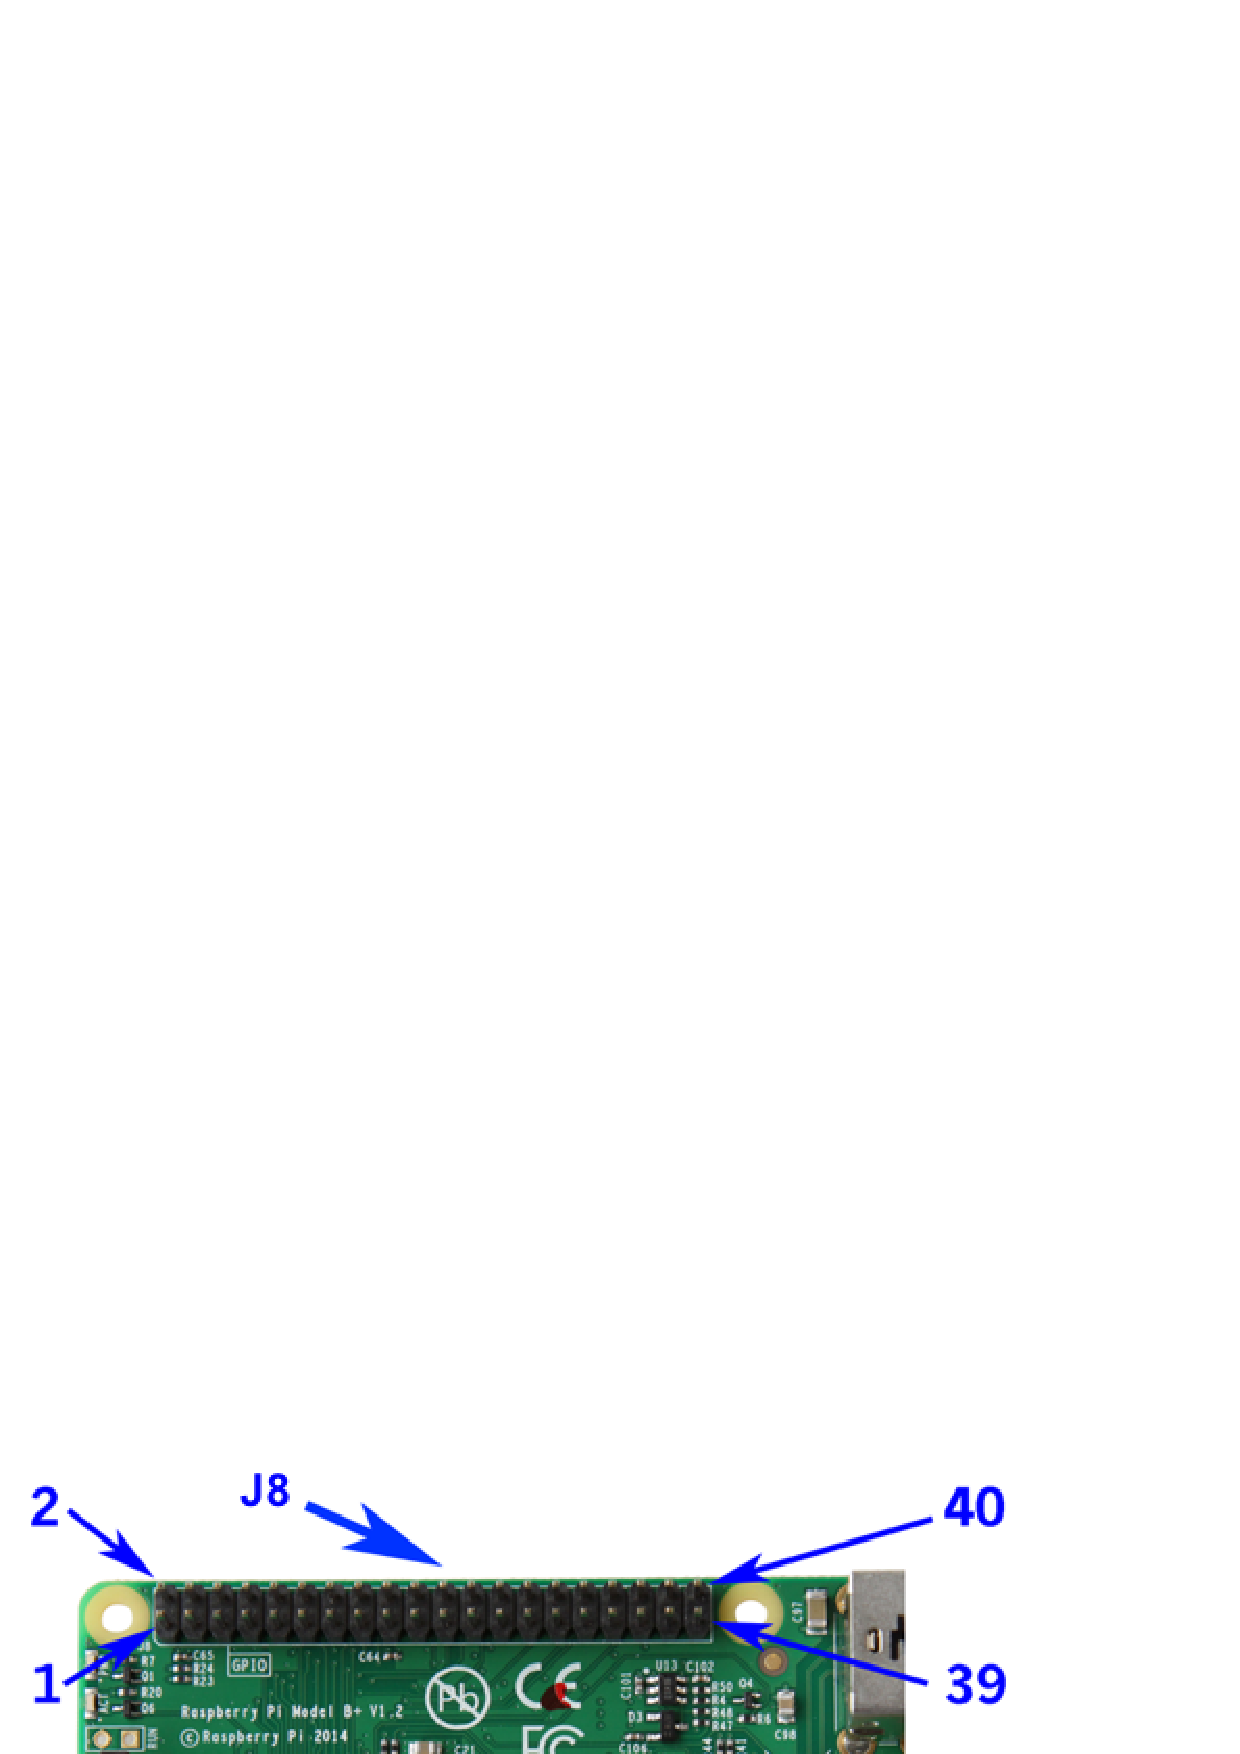
\includegraphics[width=\columnwidth]{./figs/gpio2}
\end{center}
\captionof{figure}{GPIO pin snapshot on Pi.}
\label{fig_1_3a}	
\end{figure}
%
\begin{figure}
\begin{center}
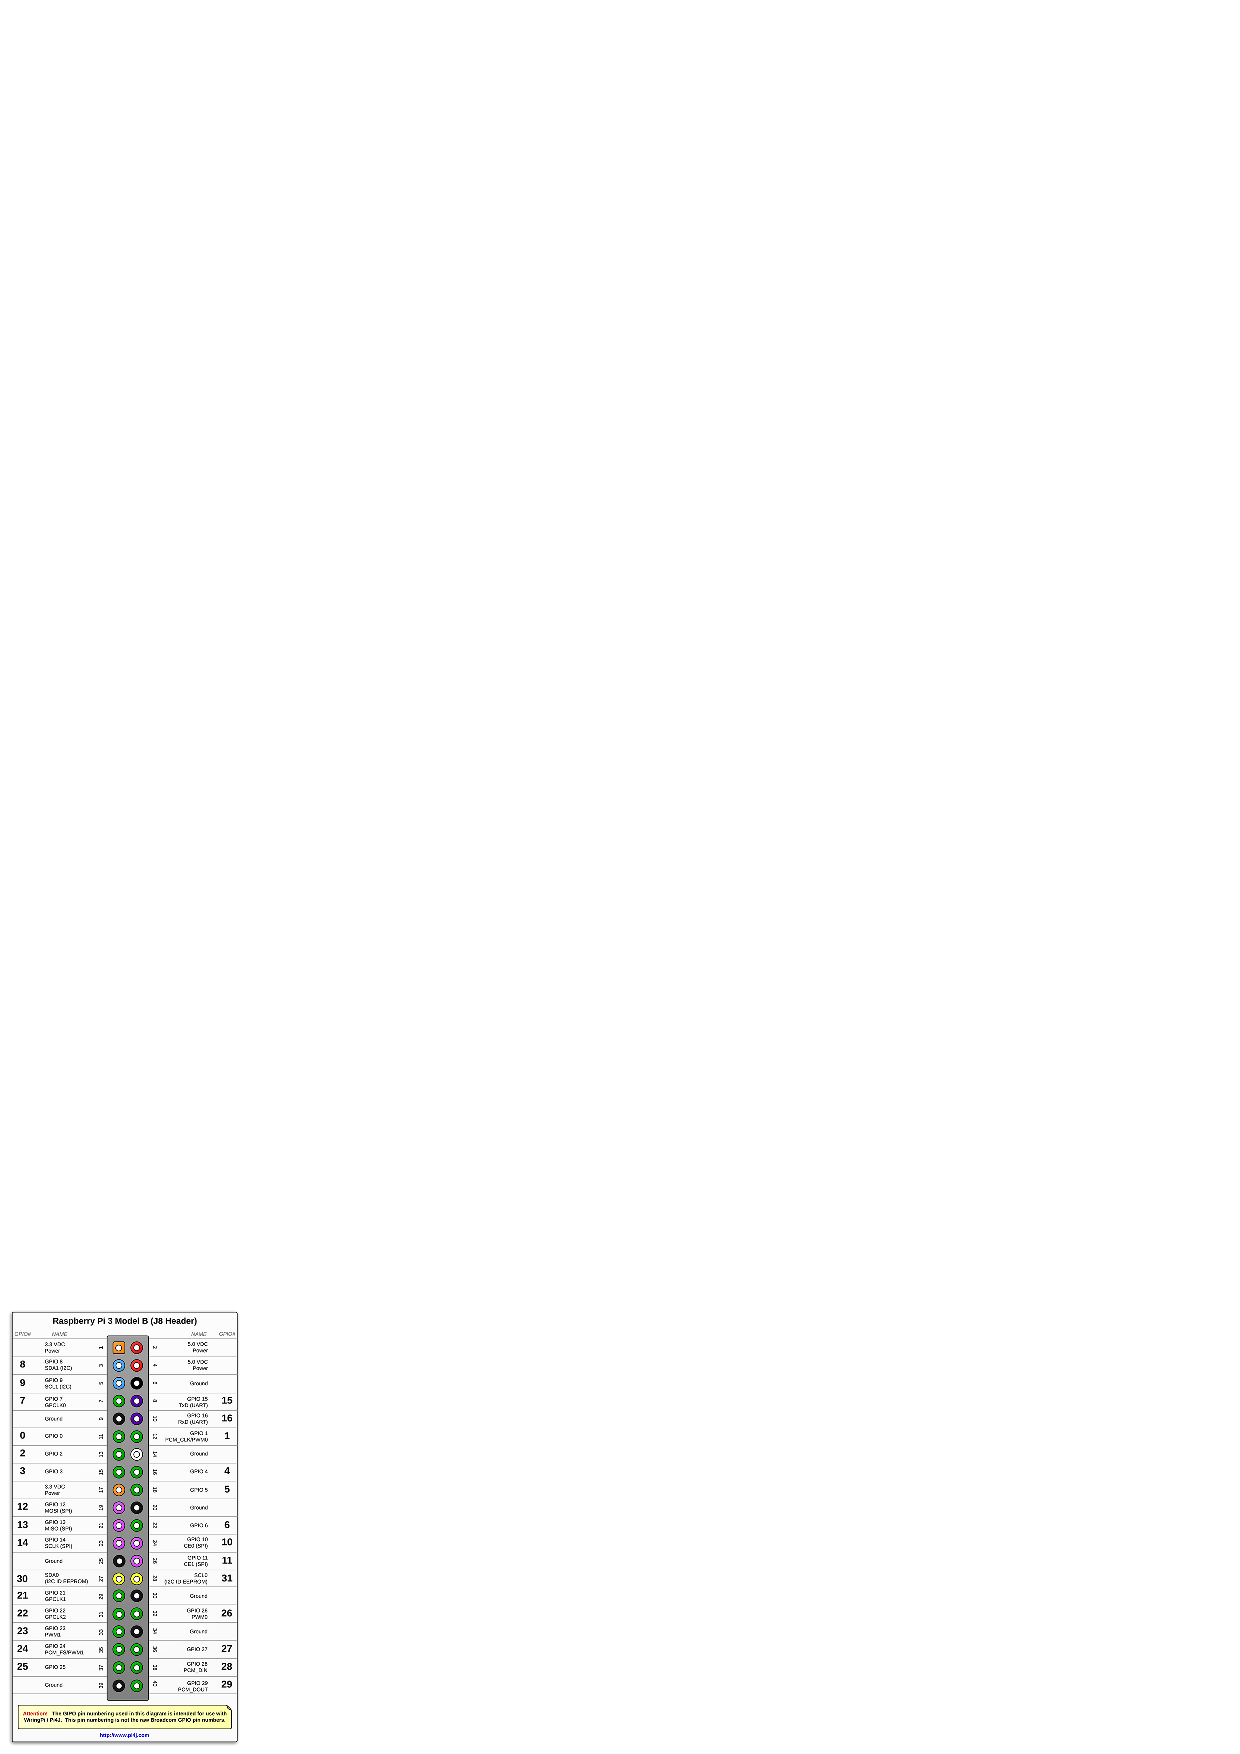
\includegraphics[width=\columnwidth]{./figs/gpio1}
\end{center}
\captionof{figure}{GPIO Wiring Pi pin configuration.}
\label{fig_1_3b}	
\end{figure}
\renewcommand{\thefigure}{\theproblem}
\begin{problem}
Connect the a-g pins of the display to the GPIO pins 0-6 of the Pi shown in \ref{fig_1_3a} and \ref{fig_1_3b}.
\end{problem}
\begin{problem}
Type the following C code and excute. What do you observe?
\end{problem}
\solution
\lstinputlisting[language=C]{./code/seven_seg_disp.c}
\begin{problem}
Now generate the numbers 0-9 by modifying the above program.
\end{problem}
\begin{problem}
Suitably modify the above program to obtain a decade counter.
\end{problem}


%\begin{problem}
%\label{prob:first_code}
%%Type the following code and execute. What do you observe?
%%\lstinputlisting[language=C]{./codes/bcd_seven.c}
%%// the setup function runs once when you press reset or power the board
int a=1,b=0,c=0,d=1,e=1,f=1,g=1;
void setup() {
    pinMode(2, OUTPUT);  
    pinMode(3, OUTPUT);
    pinMode(4, OUTPUT);
    pinMode(5, OUTPUT);
    pinMode(6, OUTPUT);
    pinMode(7, OUTPUT);
    pinMode(8, OUTPUT);            
}

// the loop function runs over and over again forever
void loop() {
  
  digitalWrite(2, a); 
  digitalWrite(3, b); 
  digitalWrite(4, c); 
  digitalWrite(5, d); 
  digitalWrite(6, e); 
  digitalWrite(7, f);     
  digitalWrite(8, g); 
}


%\end{problem}
%\begin{problem}
%Now generate the numbers 0-9 by modifying the above program.
%\end{problem}
%%
%%\newpage

%%\section{Combinational Logic}
%%
%\subsection{Counting Decoder}
	%In the  truth table in Table \ref{table:counter_decoder},  $W,X,Y,Z$ are the inputs
%and $A,B,C,D$ are the outputs. This table represents the system that increments the numbers 0-8 by 1 and resets the number 9 to 0
%%
%Note that  $D = 1$ for the inputs $0111$ and $1000$.  Using {\em boolean} logic,
%%
%\begin{equation}
%\label{bool_logic}
%D = WXYZ^{'} + W^{'}X^{'}Y^{'}Z
%\end{equation}
%%
%Note that $0111$ results in the expression $WXYZ^{'}$ and $1000$ yields $W^{'}X^{'}Y^{'}Z$. 
%%The $\&\&$ operand is used for the boolean AND (multiplication) operation, the $||$ operand is used for the OR (addition) operation and the ! operand is used for the NOT ($^{'}$) operation in Arduino code.  For example, the expression for \eqref{bool_logic} in Arudino is
%%\begin{verbatim}
%%D = (W&&X&&Y&&!Z)||(!W&&!X&&!Y&&Z);
%%\end{verbatim}

%\begin{problem}
	%\label{counter_dec}

%Write the boolean logic functions for $A,B,C$ in terms of $W,X,Y,Z$.
%\end{problem}
%%
%\input{./figs/counter_decoder}
%%
%%
%\begin{problem}
%%	\label{D_code}
%Write a program for implementing Table \ref{counter_dec}.
%%\eqref{bool_logic} in Arduino.
%\end{problem}
%%
%\solution
%%\lstinputlisting[language=C]{./codes/count_decoder.c}
%%
%%\begin{problem}
%%Modify the above program by keeping W=0,X=0,Y=0,Z=1 and A=1 and execute.  Verify that your results are consistent with Table \ref{counter_dec}.
%%\end{problem}

%\begin{problem}
%Verify if your logic is correct by observing the output on the seven segment display for different inputs.
%\end{problem}
%%
%\begin{problem}
%Connect GPIO pin 10 to the dot pin of the display and execute the following code.
%\end{problem}
%%\lstinputlisting[language=C]{./codes/blink.c}
%%
%%
%\begin{problem}
%A decade counter counts the numbers from 0-9 and then resets to 0.  Suitable modify the above programs to obtain a decade counter.
%\end{problem}

%\subsection{Display Decoder}
%%
%\begin{problem}
%Now write the truth table for the seven segment display decoder (IC 7447).  The inputs will be $A,B,C,D$ and the outputs will be $a,b,c,d,e,f,g$.
%\end{problem}
%%
%\begin{problem}
%\label{seven_seg_disp_logic}
%Obtain the logic functions for outputs $a,b,c,d,e,f,g$ in terms of the inputs $A,B,C,D$.
%\end{problem}
%\begin{problem}
%Disconnect the Pi from IC 7447 and connect the pins GPIO 0-6 in the Pi directly to the seven segment display.
%\end{problem}
%\begin{problem}
%Write a new program to implement the logic in Problem \ref{seven_seg_disp_logic} and observe the output in the display.  You have designed the logic for IC 7447!
%\end{problem}
%\begin{problem}
%Now include your counting decoder program in the  display decoder program
%and see if the display shows the consecutive number.
%\end{problem}
%A decade counter counts the numbers from 0-9 and then resets to 0.
%\begin{problem}
%Suitably modify the above program to obtain a decade counter.
%\end{problem}




%\begin{problem}
%Generate the boolean functions for the segments $a-f$ using the table in Problem \ref{bcd_ss}.  For example, the function for $a$ is obtained from the table as
%\begin{equation}
%a=\bar{D}\bar{C}\bar{B}A+\bar{D}C\bar{B}\bar{A}
%\label{boolean}
%\end{equation}
%\end{problem}
%%
%\begin{problem}
	%\label{counter_dec}
%Write functions for $A,B,C,D$ in Arduino using the following table and verify using the Arduino driven display.
		%\input{counter_decoder}
%\end{problem}
%\begin{problem}
	%Write a module for decimal to binary conversion
	%according to the example given below
	%\input{conversion}
	%%
	%$N \% 2$ gives the remainder and $N/2$ gives the quotient
%	and use it in the above code so that decimal values are given as input in the program and observed as output in the display. Note that the following code
%	\begin{verbatim}
%	a % b
%	\end{verbatim}
%	can be used to obtain the remainder when a is divided by b and
%	\begin{verbatim}
%	a/b
%	\end{verbatim}
%	gives the quotient.
%\end{problem}
 
%%
%\newpage
%\section{$M$-ary Modulation}
%\subsection{Angle Bisectors}

\begin{figure}[!h]
	\begin{center}
		
		%
\includegraphics[width=\columnwidth]{./figs/ch3_angle_bisector}
		%\vspace*{-10cm}
		\resizebox{\columnwidth}{!}{\begin{tikzpicture}
[scale=2,>=stealth,point/.style={draw,circle,fill = black,inner sep=0.5pt},]

\node (D) at (0, 0)[point,label=below :$D$] {};
\node (A) at (0, 3)[point,label=above :$A$]{};
\node (B) at (-3, 0)[point,label=below left:$B$]{};
\node (C) at (3, 0)[point,label=below right:$C$]{};
\node (O) at (0, 1.3)[point,label=below right:$O$]{};
\node (F) at (-1.1, 1.9)[point,label=above left:$F$]{};
\node (E) at (1.1, 1.9)[point,label=above right:$E$]{};

\draw (D)--(B);
\draw (B)--(A);
\draw (A)--(C);
\draw (C)--(D);
\draw [thick,dashed] (A) -- (D);
\draw [thick,dashed] (O) -- (E);
\draw [thick,dashed] (O) -- (F);
\draw (B)--(O);
\draw (C)--(O);

\tkzMarkRightAngle[size=.2](A,D,C)
\tkzMarkRightAngle[size=.15](B,F,O);
\tkzMarkRightAngle[size=.15](C,E,O);
\tkzMarkAngle[size=.4](D,B,O);
\tkzMarkAngle[size=.35](O,B,F);
\tkzMarkAngle[size=.54](E,C,O);
\tkzMarkAngle[size=.5](E,C,O);
\tkzMarkAngle[size=.6](O,C,D);
\tkzMarkAngle[size=.65](O,C,D);

\end{tikzpicture}}
	\end{center}
	\caption{Angle bisectors meet at a point}
	\label{ch3_angle_bisector}	
\end{figure}

\begin{definition}
	In Fig. \ref{ch3_angle_bisector}, $OB$ divides the  $\angle B$ into half, i.e.\begin{equation}
	\angle OBC = \angle OBA
	\end{equation}
	$OB$ is known as an angle bisector.
\end{definition}
	$OB$ and $OC$ are angle bisectors of angles $B$ and $C$. $OA$ is joined and $OD, OF$ and $OE$ are perpendiculars to sides $a,b$ and $c$.
\begin{problem}
  Show that $OD = OE = OF$.
\end{problem}
\proof In $\Delta$s $ODC$ and $OEC$,
\begin{align}
OD &= OC \sin \frac{C}{2}
\\
OE &= OC \sin \frac{C}{2} 
\\
\Rightarrow OD &=OE.
\end{align}
Similarly,
\begin{equation}
OD = OF.
\end{equation}
%
\begin{problem}
	Show that OA is the angle bisector of $\angle A$
\end{problem}
\proof In $\Delta$s $OFA$ and $OEA$,
\begin{align}
OF &= OE
\\
\Rightarrow OA \sin OAF &= OA \sin OAE \\
\Rightarrow \sin OAF &=  \sin OAE \\
\Rightarrow \angle OAF &= \angle OAE
\end{align}
which proves that $OA$ bisects $\angle A$.
{\em Conclusion:} The angle bisectors of a triangle meet at a point.


\subsection{Congruent Triangles}
%
\begin{problem}
	Show that in $\Delta$s $ODC$ and $OEC$, corresponding sides and angles are equal.
\end{problem}
\begin{definition}
	Note that    $\Delta$s $ODC$ and $OEC$ are known as congruent triangles.  To show that two triangles are congruent, it is sufficient to show that some angles and sides are equal.
\end{definition}
\begin{problem}
SSS:	Show that if the corresponding sides of three triangles are equal, the triangles are congruent.
\end{problem}
\begin{problem}
ASA:	Show that if two angles and any one side  are equal in corresponding triangles, the triangles are congruent.
\end{problem}
\begin{problem}
SAS:	Show that if two sides and the angle between them are equal in corresponding triangles, the triangles are congruent.
\end{problem}
\begin{problem}
RHS:	For two right angled triangles, if the hypotenuse and one of the sides are equal, show that the triangles are congruent.
\end{problem}
	%
%%
\subsection{Perpendicular Bisectors}
\begin{definition}
	In Fig. \ref{ch3_perp_bisector}, OD $\perp BC$ and $BD=DC$. $OD$ is defined as the perpendicular bisector of $BC$.
\end{definition}

\begin{problem}
	In Fig. \ref{ch3_perp_bisector}, show that $OA=OB=OC$.
\end{problem}
%%
%%
\begin{figure}[!h]
	\begin{center}
		
		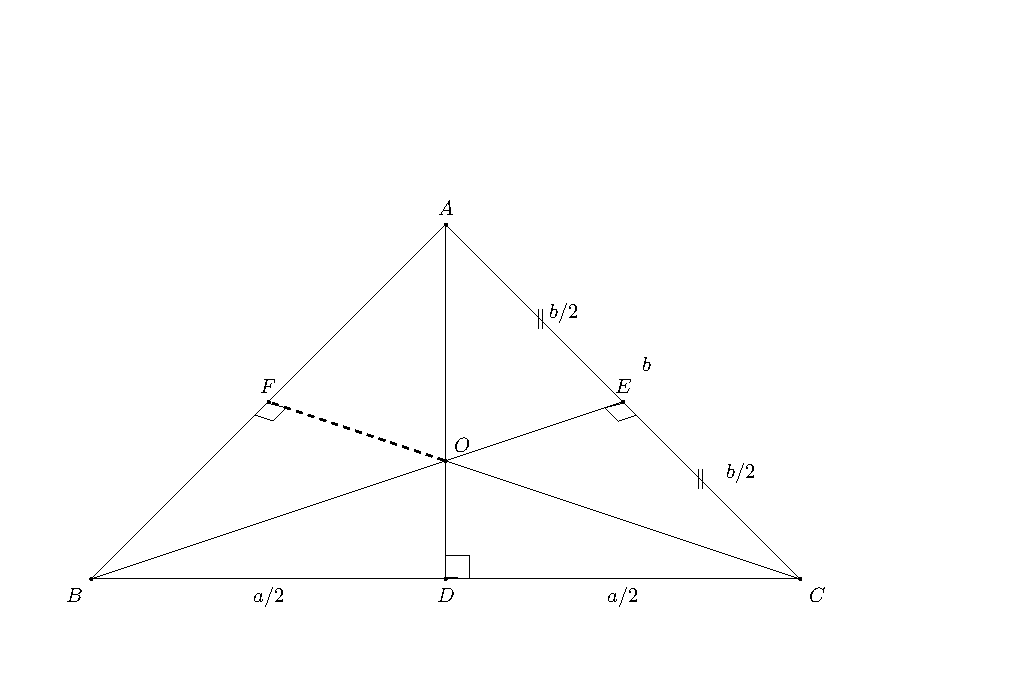
\includegraphics[width=\columnwidth]{./figs/fig_3.8.eps}
%		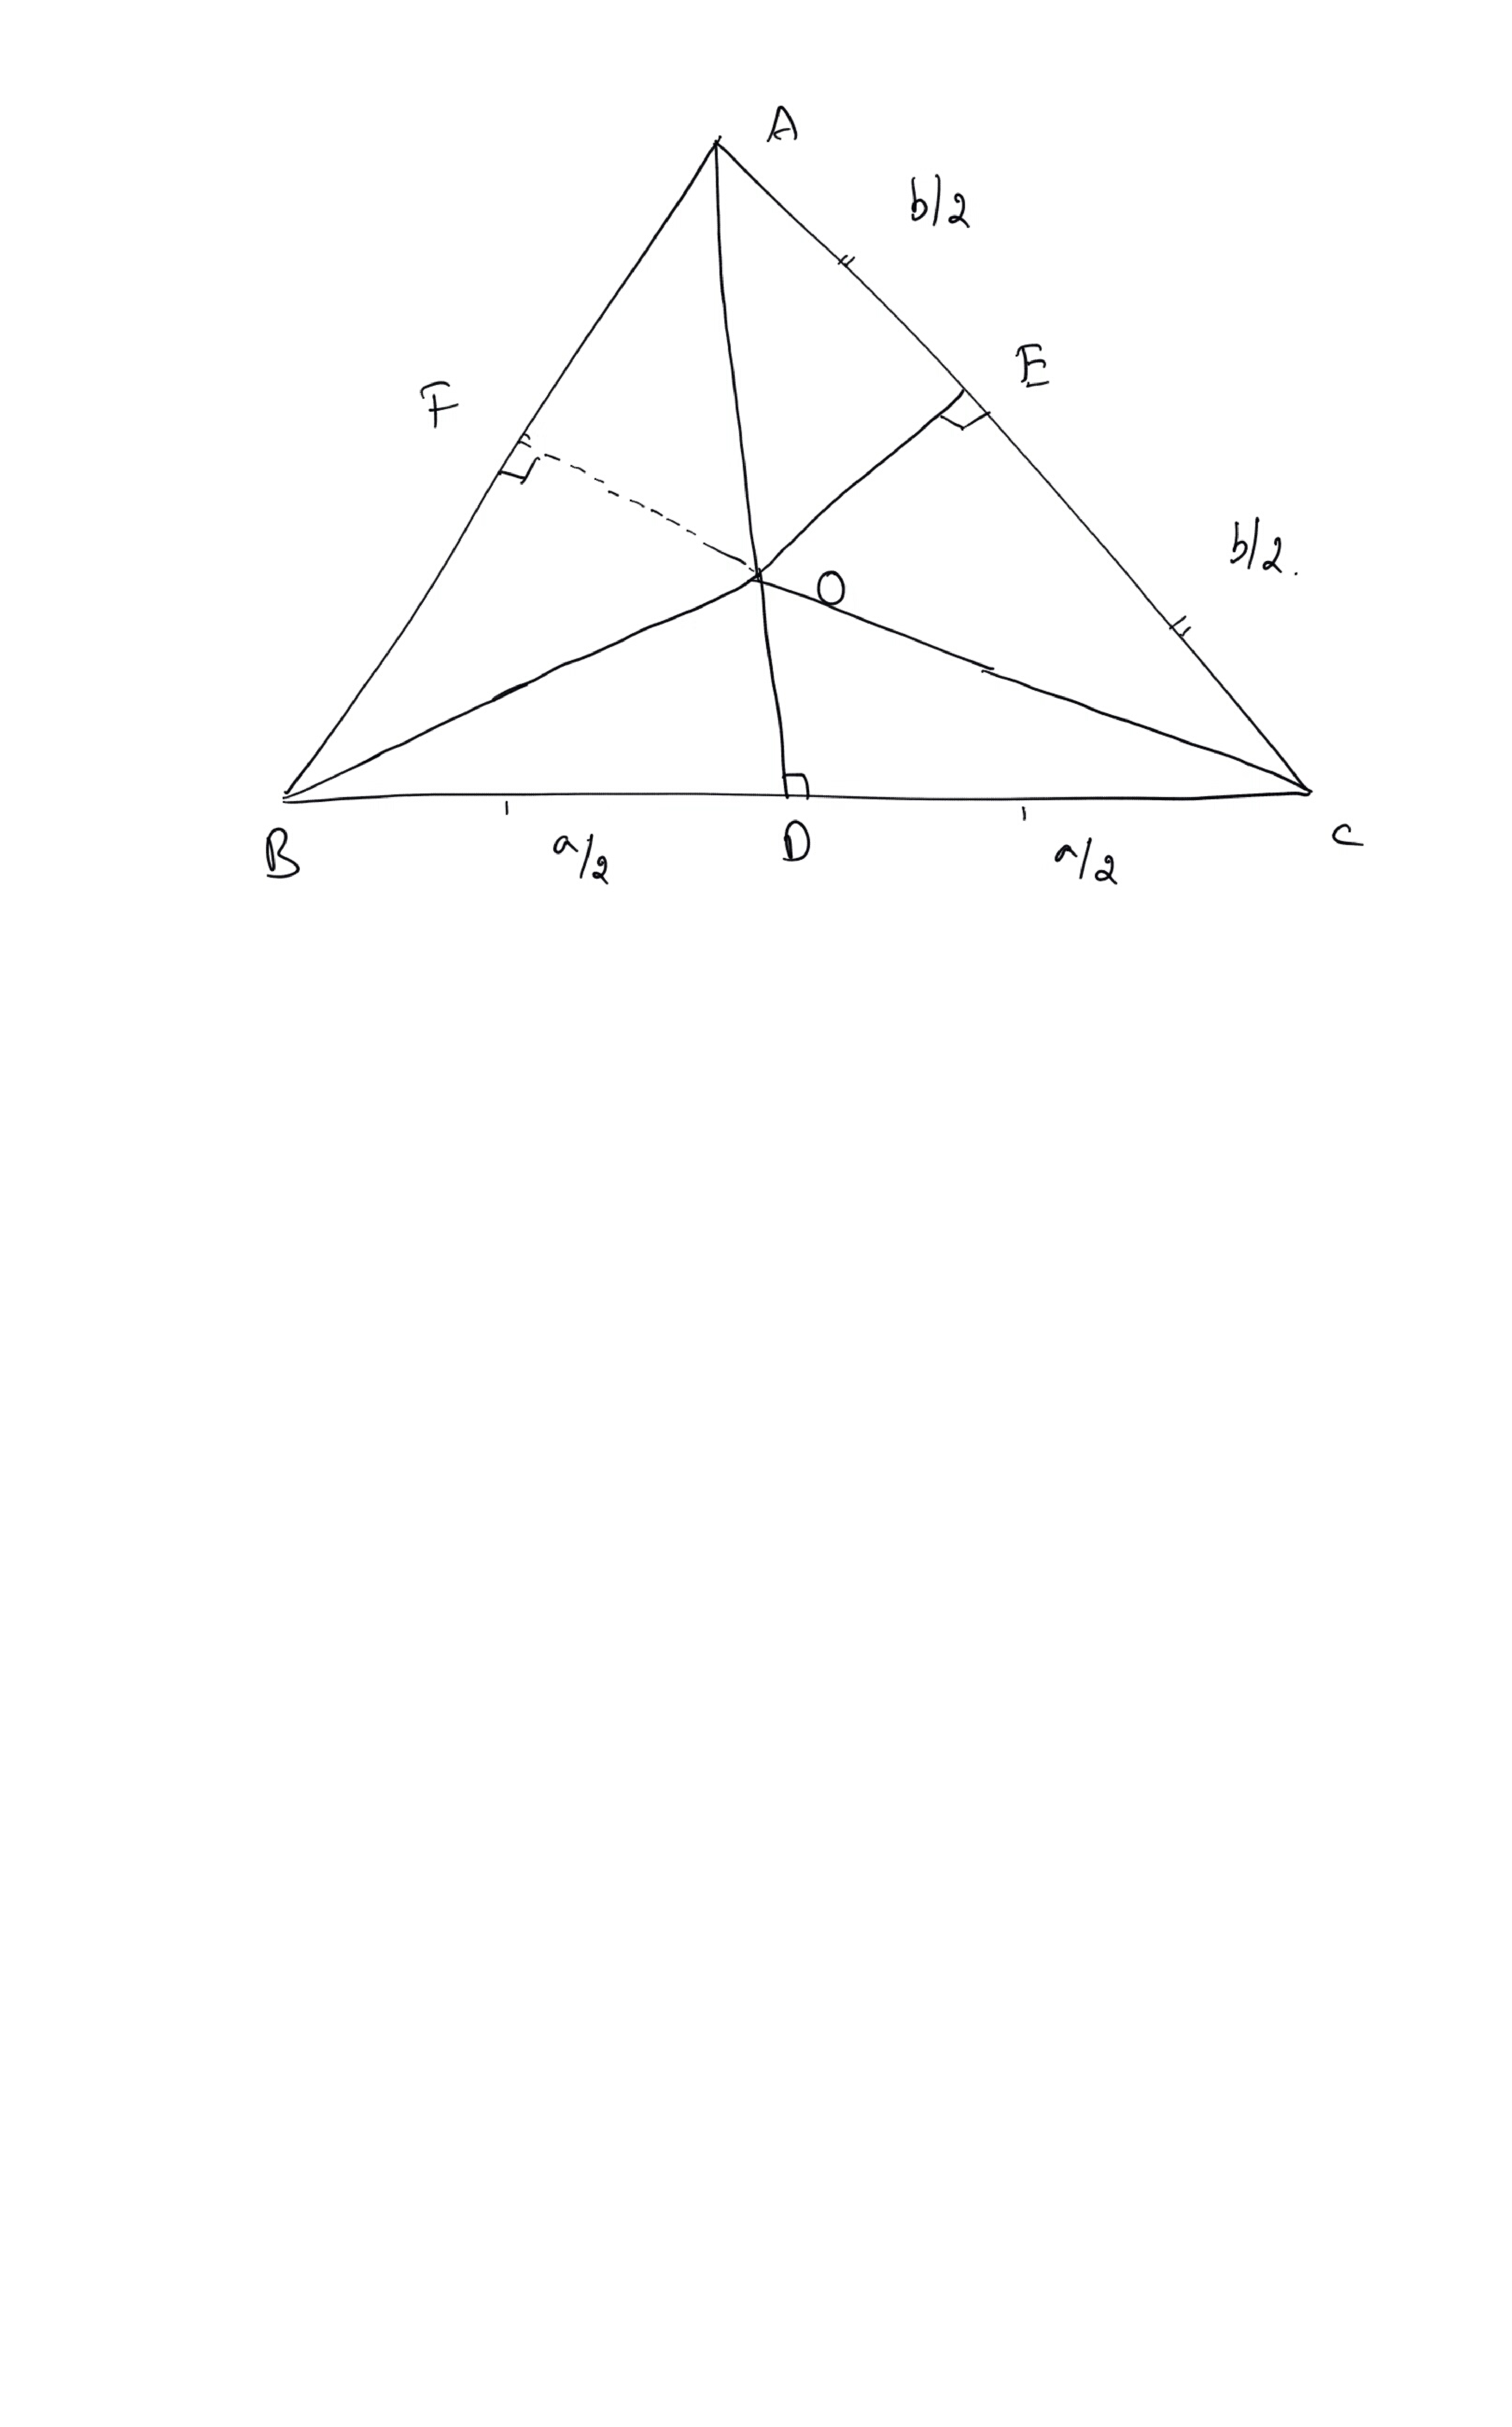
\includegraphics[width=\columnwidth]{./figs/ch3_perp_bisector}
		%\vspace*{-10cm}
%		\resizebox{\columnwidth}{!}{\documentclass{standalone}
\usepackage{tikz}
\usepackage{tkz-euclide}
\usetkzobj{all}
%\usepackage{amsmath}
\providecommand{\brak}[1]{\ensuremath{\left(#1\right)}}

\begin{document}
\begin{tikzpicture}
[scale=2,>=stealth,point/.style={draw,circle,fill = black,inner sep=0.5pt},]

\node (E) at (1.5, 1.5)[point,label=above :$E$] {};
\node (F) at (-1.5, 1.5)[point,label=above :$F$] {};
\node (A) at (0, 3)[point,label=above :$A$]{};
\node (B) at (-3, 0)[point,label=below left:$B$]{};
\node (C) at (3, 0)[point,label=below right:$C$]{};
\node (D) at (0,0)[point,label=below :$D$] {};
\node (O) at (0,1)[point,label=above right :$O$] {};


\draw (B)--(A);
\draw (A)--(C);
\draw (B)--(C);
\draw (B)--(E);
\draw (C)--(O);
\draw (A)--(D);
\draw [thick,dashed] (O) -- (F);

\node [above] at (1.7,1.7) {$b$};
\node [above] at (2.5,.75) {$b/2$};
\node [above] at (1,2.1) {$b/2$};
\node [above] at (-1.5,-0.3){$a/2$};
\node [above] at (1.5,-0.3){$a/2$};
\tkzMarkRightAngle[size=.16](B,F,O)
\tkzMarkRightAngle[size=.16](C,E,O)
\tkzMarkRightAngle[size=.2](A,D,C)
\draw   -- (4.3,1.7) node[midway] {$\parallel$};
\draw   -- (1.6,4.4) node[midway] {$\parallel$};

\end{tikzpicture}
\end{document}}
	\end{center}
	\caption{Perpendicular bisectors meet at a point}
	\label{ch3_perp_bisector}	
\end{figure}
%
\proof In $\Delta$s $ODB$ and $ODC$, using Budhayana's theorem,
%
\begin{equation}
\begin{split}
OB^2 &= OD^2 + BD^2 \\
OC^2 &= OD^2 + DC^2 
\end{split}
\end{equation}
%
Since $BD = DC = \frac{a}{2}$, $OB = OC$.  Similarly, it can be shown that $OA = OC$.  Thus, $OA=OB=OC$.
%
\begin{definition}
	In $\Delta AOB$, $OA = OB$.  Such a triangle is known as an isoceles triangle.
\end{definition}
%
\begin{problem}
	Show that $AF = BF$.
\end{problem}
\proof Trivial using Budhayana's theorem.  This shows that $OF$ is a perpendicular bisector of $AB$. 
{\em Conclusion:}  The perpendicular bisectors of a triangle meet at a point.
%
\subsection{Perpendiculars from Vertex to Opposite Side}
	%
	%
	In Fig. \ref{ch3_perp_triang}, $AD \perp BC$ and $BE \perp AC$. $CF$ passes through $O$ and meets
	$AB$ at $F$.  	
\begin{problem}
	Show that 
	\begin{align}
	OE = c \cos A \cot C
	\end{align}
\end{problem}
	\begin{figure}[!h]
		\begin{center}
			
			%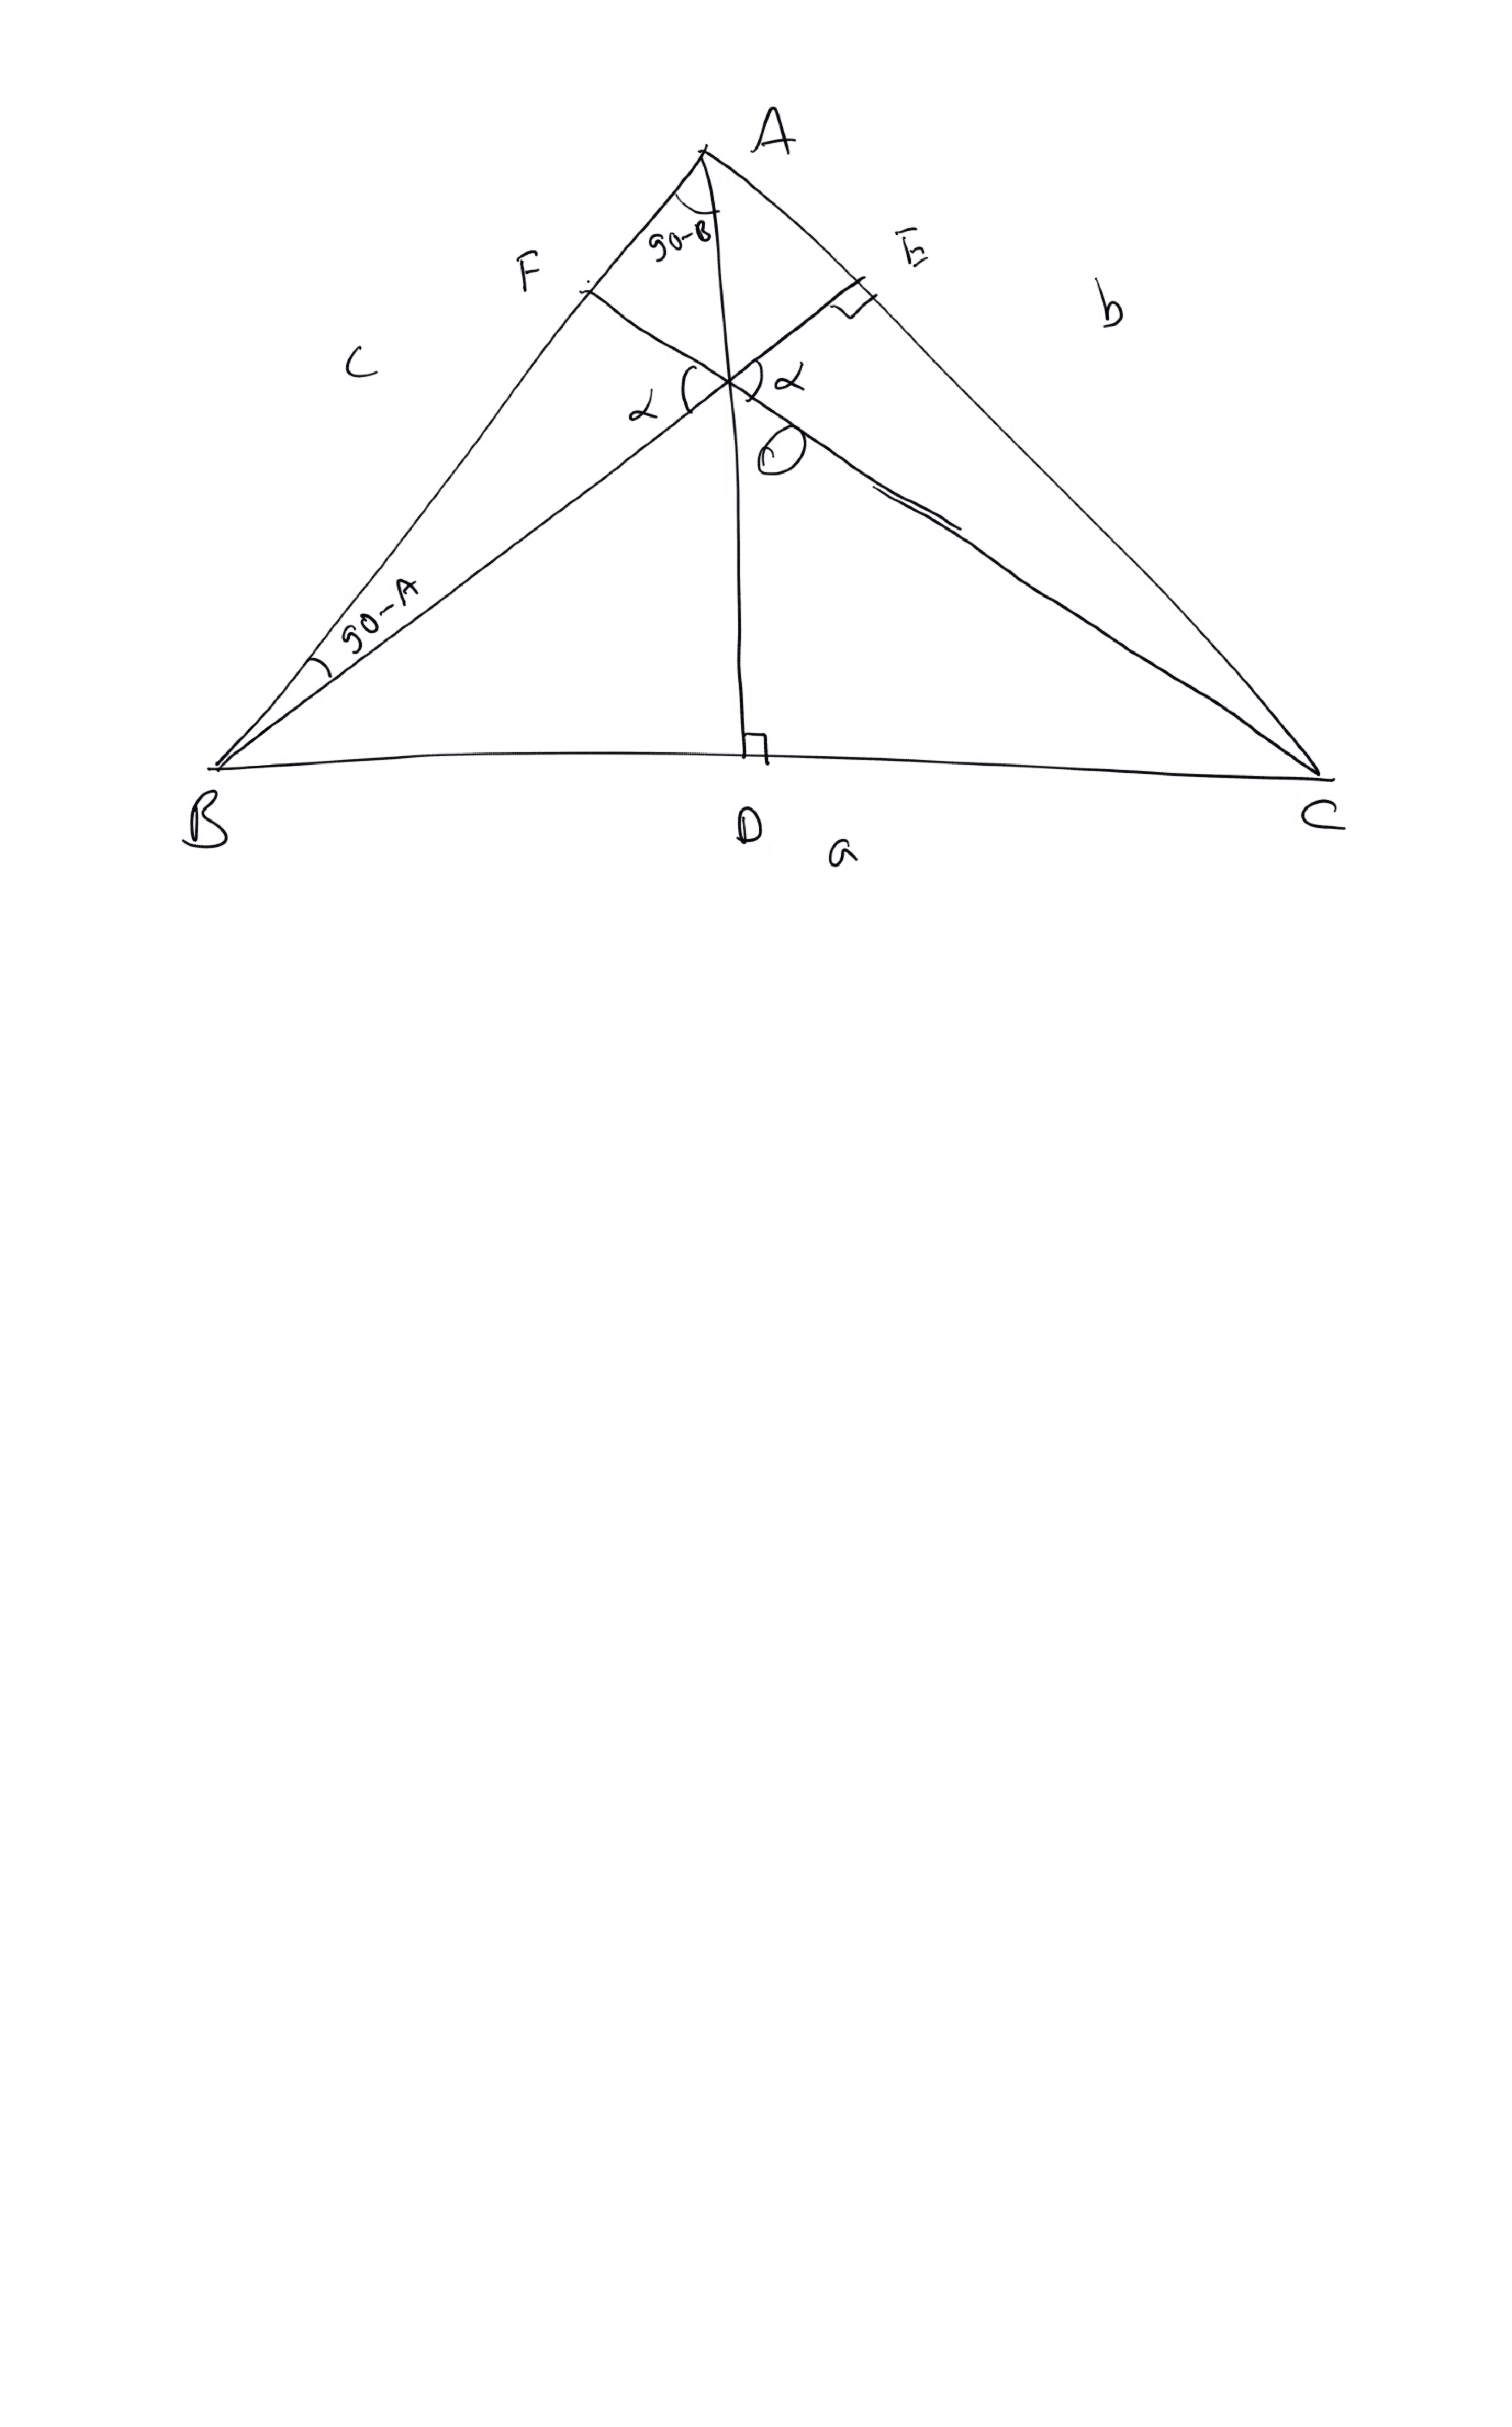
\includegraphics[width=\columnwidth]{./figs/ch3_perp_triang}
			%\vspace*{-10cm}
			\resizebox{\columnwidth}{!}{\begin{tikzpicture}
[scale=2,>=stealth,point/.style={draw,circle,fill = black,inner sep=0.5pt},]

\node (E) at (1.5, 1.5)[point,label=above :$E$] {};
\node (F) at (-1.5, 1.5)[point,label=above :$F$] {};
\node (A) at (0, 3)[point,label=above :$A$]{};
\node (B) at (-3, 0)[point,label=below left:$B$]{};
\node (C) at (3, 0)[point,label=below right:$C$]{};
\node (O) at (0,1)[point,label=above right :$O$] {};
\node (D) at (0,0)[point,label=below :$D$] {};


\draw (B)--(A);
\draw (A)--(C);
\draw (B)--(E);
\draw (C)--(F);
\draw (B)--(C);
\draw (A)--(D);

\node [below] at (0,-0.3) {$a$};
\node [above] at (-1.7,1.7) {$c$};
\node [above] at (1.7,1.7) {$b$};
\node [above] at (1,1.3) {$p$};
\node [above] at (-1,1.3) {$q$};
\node [above] at (-2.3,0.24){\rotatebox{45}{$90-A$}};
\node [above] at (-0.4,2.1) {\rotatebox{45}{$90-B$}};
\node [above] at (0.4,2.1) {\rotatebox{-45}{$90-C$}};

\tkzMarkAngle[size=.3](F,O,B);
\tkzMarkAngle[size=.3](C,O,E);
\tkzMarkAngle[size=.4](O,B,F);
\tkzMarkAngle[size=.2](F,A,O);
\tkzMarkAngle[size=.3](O,A,E);
\draw (-0.5,1) node{$\alpha$};
\draw (0.5,1) node{$\alpha$};

\end{tikzpicture}
}
		\end{center}
		\caption{Perpendiculars from vertex to opposite side meet at a point}
		\label{ch3_perp_triang}	
	\end{figure}
%
\proof In $\Delta$ s $AEB$ and $AEO$,
%
\begin{align}
AE &= c \cos A \\
OE &= AE \tan \brak{90^{\degree} - C} \brak{\because ADC \text{ is right angled}} \\
&= AE \cot C
\end{align}
%
From both the above, we get the desired result.
%
\begin{problem}
	Show that $\alpha = A$.
\end{problem}
\proof In $\Delta OEC$,
%
\begin{equation}
CE = a \cos C \brak{\because BEC \text{ is right angled}}
\end{equation}
%
Hence,
%
\begin{equation}
\begin{split}
\tan \alpha &= \frac{CE}{OE} \\
&=  \frac{a \cos C}{c \cos A \cot C} \\
&=  \frac{a \cos C \sin C}{c \cos A \cos C} \\
&= \frac{a \sin C}{c \cos A } \\
&= \frac{c \sin A}{c \cos A } \brak{\because \frac{a}{\sin A} = \frac{c}{\sin C}}\\
&= \tan A\\
\Rightarrow \alpha = A
\end{split}
\end{equation}
%
\begin{problem}
	Show that $CF \perp AB$
\end{problem}
\proof Consider triangle OFB and the result of the previous problem.  $\because$ the sum of the angles of a triangle is $180^{\degree}$, $\angle CFB = 90^{\degree}$.
{\em Conclusion: The perperdiculars from the vertex of a triangle to the opposite side meet at a point.} 
%
%\newpage
%\section{BER in Rayleigh Flat Slowly Fading Channels}
	%\subsection{Chord of a Circle}

\begin{figure}[!h]
	\begin{center}
		
		
\includegraphics[width=\columnwidth]{./figs/ch4_circle_def}
		\vspace*{-10cm}
	\end{center}
	\caption{Circle Definitions}
	\label{ch4_circle_def}	
\end{figure}
\begin{definition}
	Fig. \ref{ch4_circle_def} represents a circle.  The points in the circle are at a distance $r$ from the centre $O$.  $r$ is known as the radius.
\end{definition}

\subsection{Chords of a circle}
\begin{definition}
	In Fig. \ref{ch4_circle_def}, $A$ and $B$ are points on the circle.  The line $AB$ is known as a chord of the circle.
\end{definition}
%
%
\begin{problem}
	\label{ch4_prob_circle_subtend}
	In Fig. \ref{ch4_circle_subtend}  Show that $\angle OAB = 2\angle APB $.
\end{problem}
\begin{figure}[!h]
	\begin{center}
		
		
\includegraphics[width=\columnwidth]{./figs/ch4_circle_subtend}
		\vspace*{-10cm}
	\end{center}
	\caption{Angle subtended by chord $AB$ at the centre $O$ is twice the angle subtended at $P$. }
	\label{ch4_circle_subtend}	
\end{figure}

\proof In Fig. \ref{ch4_circle_subtend}, the triangeles $OPA$ and $OPB$ are isosceles. Hence,
%
\begin{align}
\angle OPB = \angle OBP &= \theta_1 \\
\angle OPA = \angle OAP &= \theta_2
\end{align}
%
Also, $\alpha$ and $\beta$ are exterior angles corresponding to the triangle $OPB$ and $OPA$ respectively. Hence
%
\begin{align}
\alpha &= 2\theta_1 \\
\beta &= 2\theta_2
\end{align}
%
Thus,
%
\begin{align}
\angle AOB &= \alpha + \beta \\
&= \theta_1 + \theta_2 \\
&= \angle APB
\end{align}
%
\begin{definition}
	The diameter of a circle is the chord that divides the circle into two equal parts. In Fig. \ref{ch4_circle_dia}, $AB$ is the diameter and passes through the centre $O$
\end{definition}
%
\begin{problem}
In Fig. \ref{ch4_circle_dia}, show that $\angle APB = 90^{\degree}$ .
\end{problem}
%
\begin{figure}[!h]
	\begin{center}
		
		
\includegraphics[width=\columnwidth]{./figs/ch4_circle_dia}
		\vspace*{-10cm}
	\end{center}
	\caption{Diameter of a circle.}
	\label{ch4_circle_dia}	
\end{figure}

\begin{problem}
	In Fig. \ref{ch4_chord_product}, show that 
	\begin{equation}
	\begin{split}
\angle ABD &= \angle ACD \\
\angle CAB &= \angle CDB	
	\end{split}
	\end{equation}
\end{problem}
\begin{figure}[!h]
	\begin{center}
		
		
\includegraphics[width=\columnwidth]{./figs/ch4_chord_product}
		\vspace*{-10cm}
	\end{center}
	\caption{$PA.PB = PC.PD$}
	\label{ch4_chord_product}	
\end{figure}
%
%
\proof Use Problem \ref{ch4_prob_circle_subtend}.
%
\begin{problem}
	In Fig. \ref{ch4_chord_product}, show that the triangles $PAB$ and $PBD$ are similar
\end{problem}
\proof Trivial using previous problem
\begin{problem}
	In Fig. \ref{ch4_chord_product}, show that 
	\begin{equation}
	PA.PB = PC.PD
	\end{equation}
\end{problem}
%
\proof Since triangles $PAC$ and $PBD$ are similar, 
%
\begin{align}
\frac{PA}{PD} &= \frac{PC}{PB} \\
\Rightarrow PA.PB &= PC.PD
\end{align}
%
%
\begin{definition}
	The line $PX$ in Fig. \ref{ch4_tangent_def} touches the circle at exactly one  point $P$. It is known as the tangent to the circle.
\end{definition}
%
%
\begin{problem}
	$OP$ is the perpendicular to the line $PX$ as shown in the Fig. \ref{ch4_short_dist}. Show that $OP$ is the shortest distance between the point $O$ and the line $PX$. 
\end{problem}
\proof Let $P_1$ be a point on the line $PX$. Then $OPP_1$ is a right angled triangle.  Using Budhayana's theorem,
%
\begin{figure}[!h]
	\begin{center}
		
		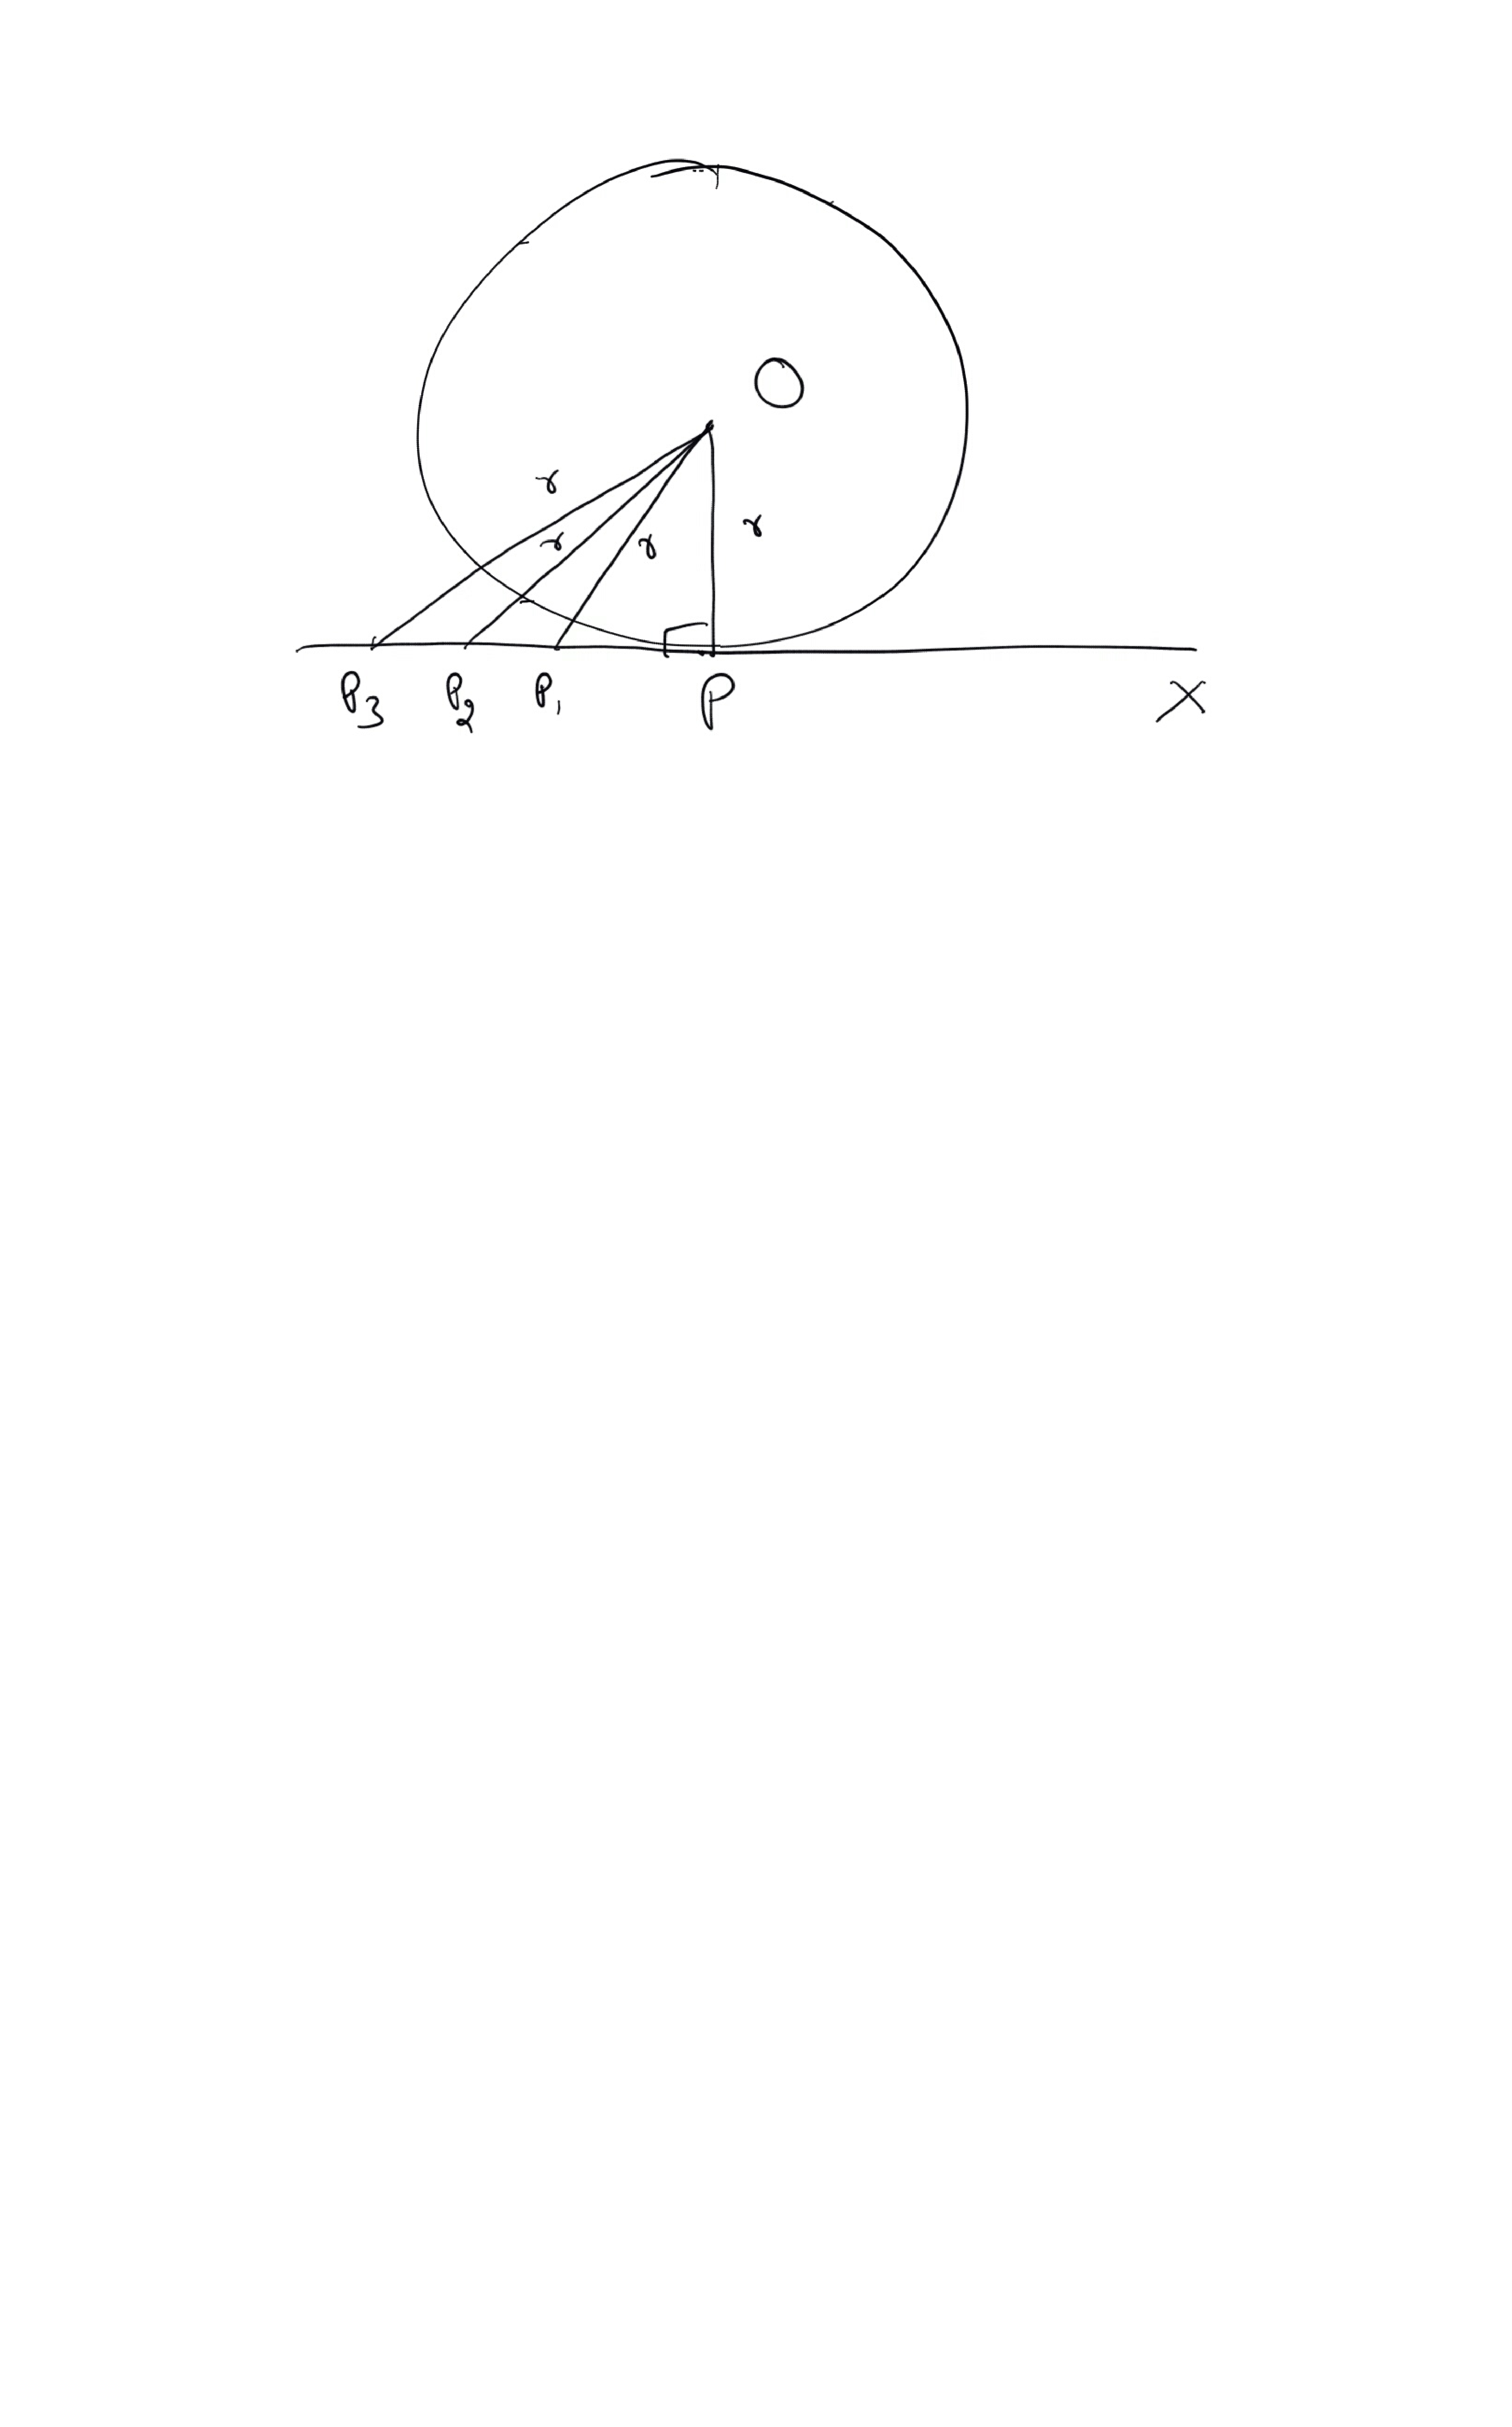
\includegraphics[width=\columnwidth]{./figs/ch4_tangent_def}
		\vspace*{-10cm}
	\end{center}
	\caption{Tangent to a Circle.}
	\label{ch4_tangent_def}	
\end{figure}
%
\begin{figure}[!h]
	\begin{center}
		
		
\includegraphics[width=\columnwidth]{./figs/ch4_short_dist}
		\vspace*{-10cm}
	\end{center}
	\caption{Shortest distance from $O$ to line $PX$}
	\label{ch4_short_dist}	
\end{figure}

%
\begin{equation}
\begin{split}
OP_1^2 &= OP^2 + PP_1^2 \\
\Rightarrow OP_1 > OP
\end{split}
\end{equation}
%
Thus, $OP$ is the shortest distance between $O$ and line $PX$.
%
\begin{problem}
Show that $\angle OPX = 90 ^{\degree}$
\end{problem}
\proof In Fig. \ref{ch4_tangent_def}, we can see that $OP$ is is the radius of the circle and the length of all line segments from $O$ to the line $PX > r$.  Using the result of the previous 
problem, it is obvious that $OP \perp PX$. 
%
	%
\begin{problem}
In Fig. \ref{ch4_tangent_prod} show that 
%
\begin{equation}
\angle PCA = \angle PBC
\end{equation}
%
$O$ is the centre of the circle and $PC$ is the tangent.
\end{problem}
	\begin{figure}[!h]
		\begin{center}
			
			
\includegraphics[width=\columnwidth]{./figs/ch4_tangent_prod}
			\vspace*{-10cm}
		\end{center}
		\caption{$PA.PB = PC^2$.}
		\label{ch4_tangent_prod}	
	\end{figure}
	%

%
\proof For convenience, greek letters are used for representing certain angles. Since $\Delta OAC$ is isosceles,
%
\begin{align}
2 \alpha + 2 \brak{\beta - \phi} &= 180^{\degree} \\
\Rightarrow  \alpha +  \brak{\beta - \phi} &= 90^{\degree} \\
\Rightarrow  \alpha +  \beta  &= 90^{\degree} + \phi
\end{align}
%
Since $theta$ is an exterior angle for the $\Delta ABC
$,
%
\begin{equation}
\theta = \alpha + \beta
\end{equation}
%
From both the above equations
%
\begin{equation}
\theta = 90^{\degree} + \phi
\end{equation}
%
Since PC is the tangent, 
%
\begin{equation}
\angle PCB = 90^{\degree} + \phi = \theta
\end{equation}
%
Considering the sum of angles in $\Delta PAC$ $\Delta PBC$,
%
\begin{align}
\angle P + \theta + \angle PCA &= 180^{\degree} \\
\angle P + \theta + \alpha &= 180^{\degree}
\end{align}
Hence,
%
\begin{equation}
\angle PCA = \alpha
\end{equation}
%
\begin{problem}
	In Fig. \ref{ch4_tangent_prod}, show that the triangles $PAC$ and $PBC$ are similar.
\end{problem}
\proof From the previous problem, it is obvious that corresponding angles of both triangles are equal.  Hence they are similar.
%
\begin{problem}
	Show that $PA.PB = PC^2$
\end{problem}
\proof Since $\Delta PAC \sim \Delta PBC$, their sides are in the same ratio.  Hence,
%
\begin{align}
\frac{PA}{PC} &= \frac{PC}{PB} \\
\Rightarrow PA.PB &=PC^2
\end{align}
%
%
\begin{problem}
	In Fig. \ref{ch4_chord_tangent_prod}, show that\begin{equation}
	PA.PB = PC.PD
	\end{equation}
\end{problem}
%
\begin{figure}[!h]
	\begin{center}
		
		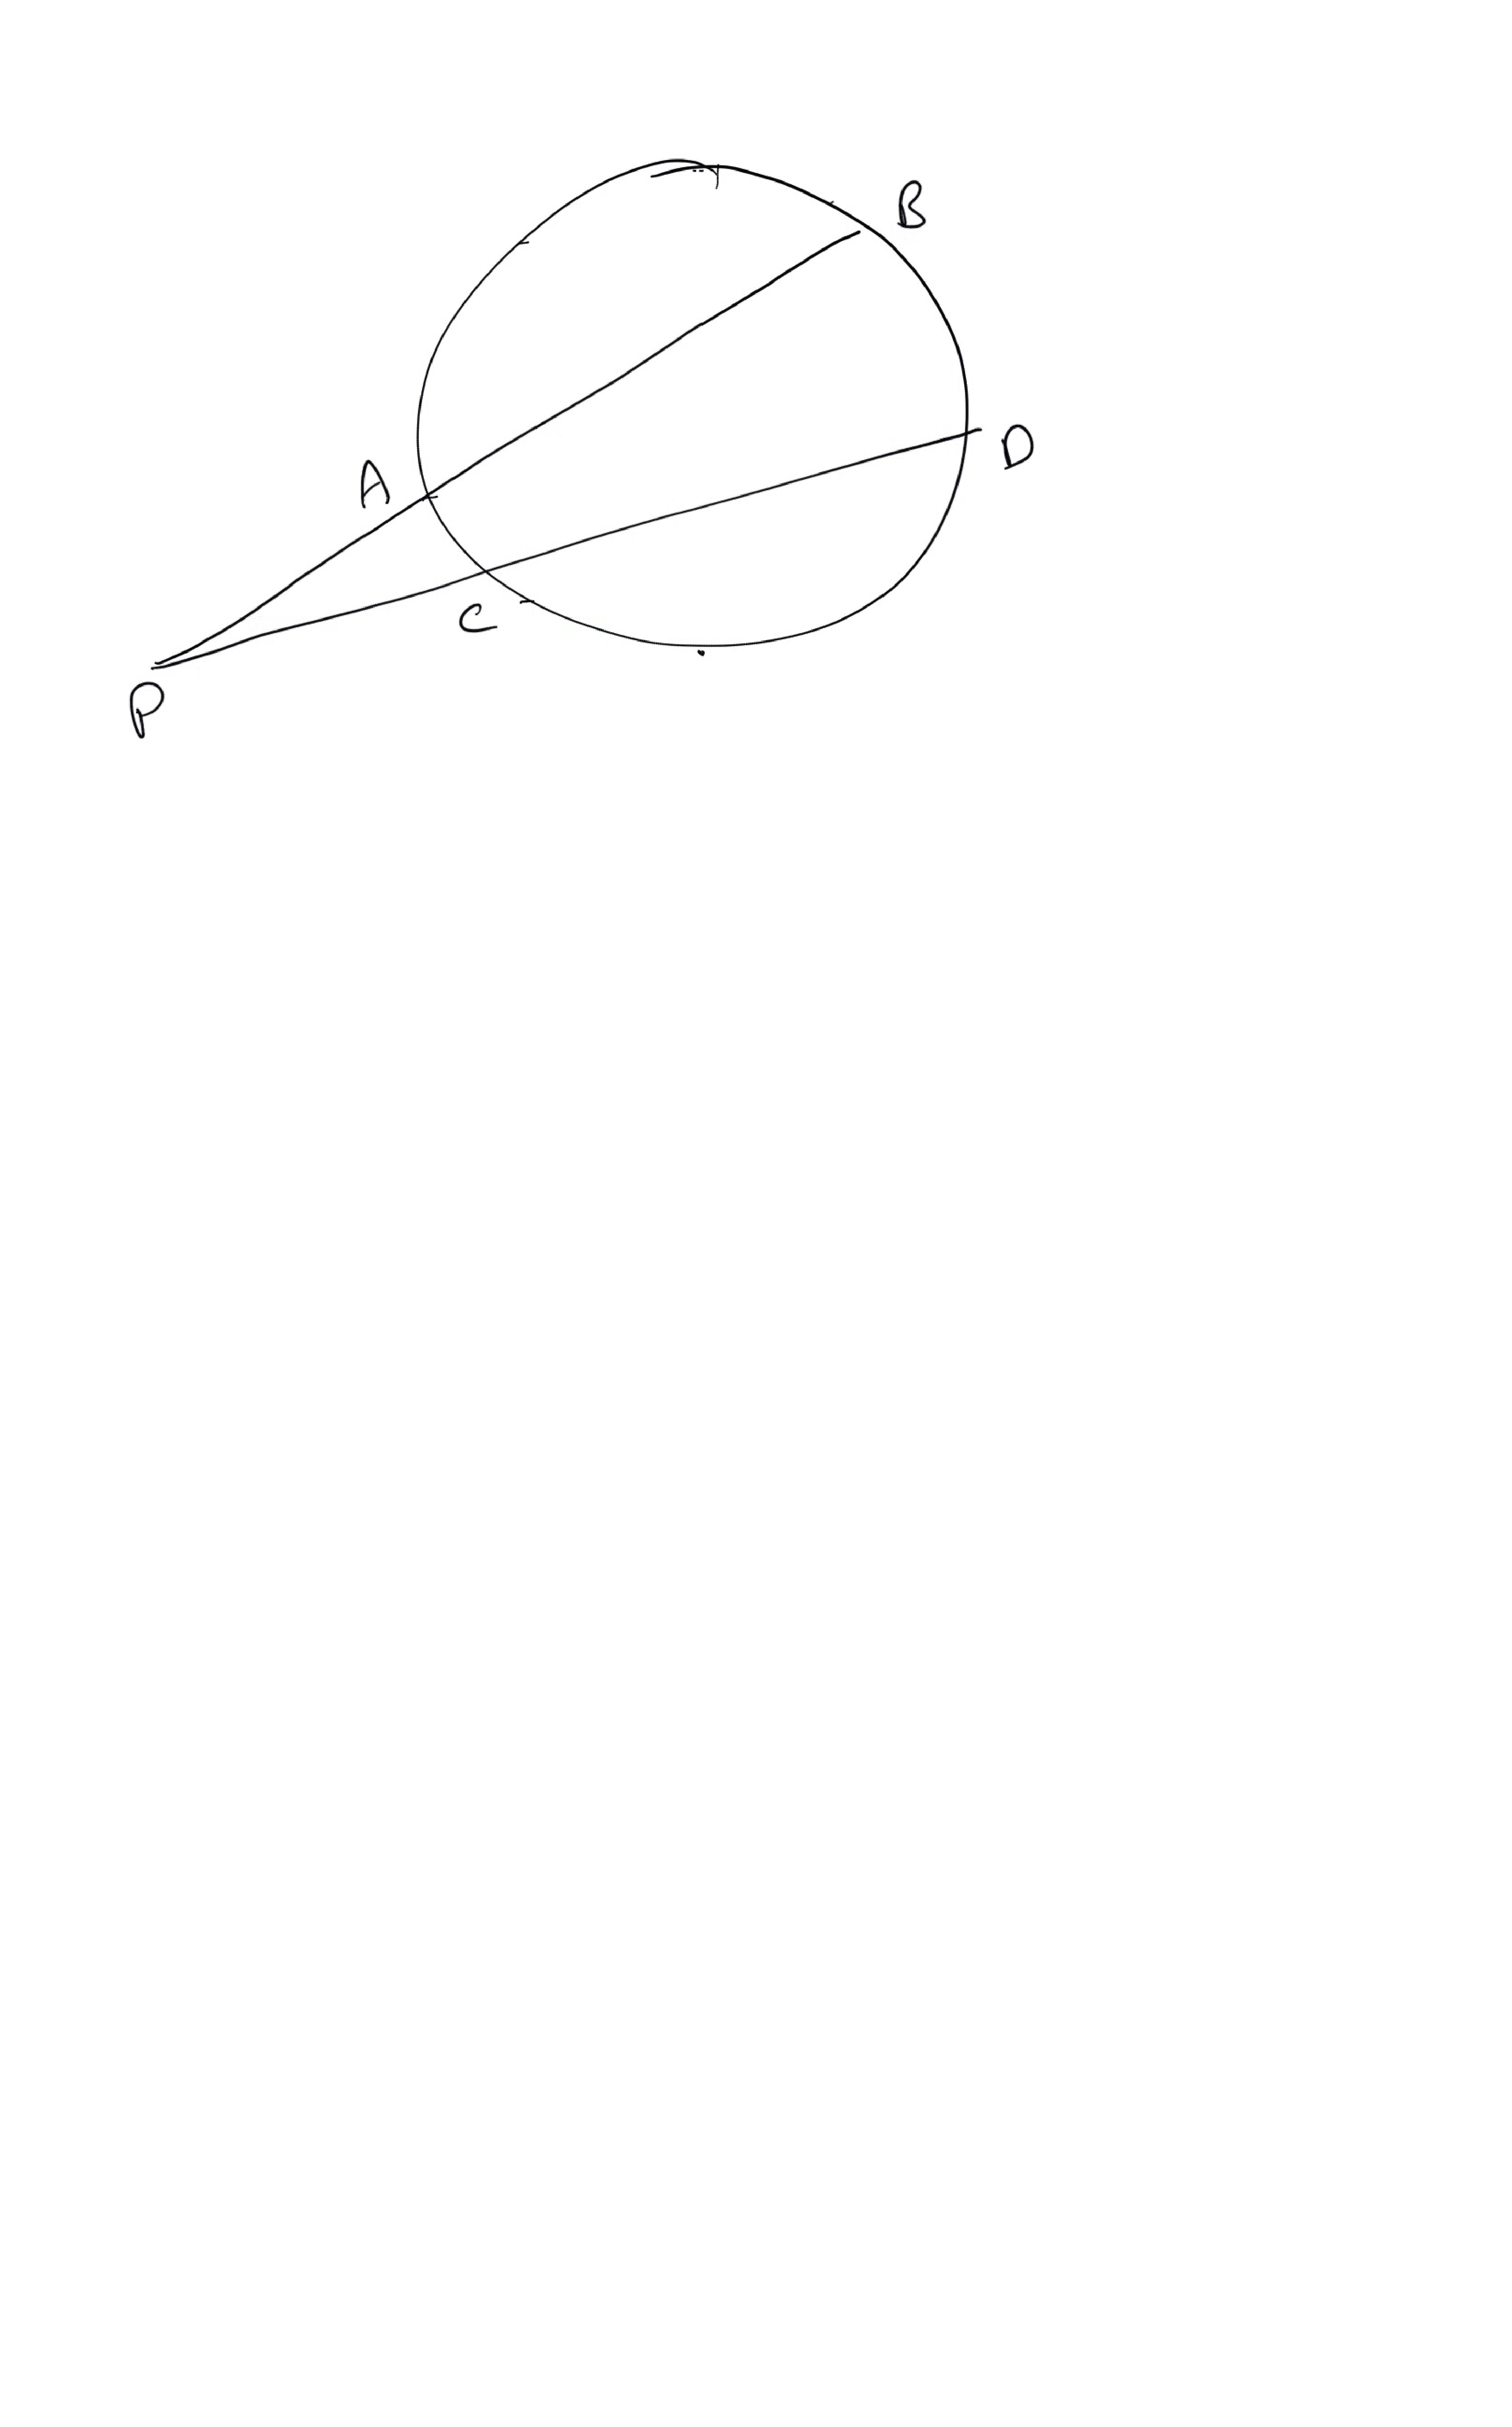
\includegraphics[width=\columnwidth]{./figs/ch4_chord_tangent_prod}
		\vspace*{-10cm}
	\end{center}
	\caption{$PA.PB = PC^2$.}
	\label{ch4_chord_tangent_prod}	
\end{figure}

\proof Draw a tangent and use the previous problem.
 

\end{document}


